% PREAMBLE

\documentclass[12pt]{scrreprt}

\usepackage[a4paper]{geometry}
\usepackage{graphicx,color}
\usepackage[numbers,sort&compress]{natbib}
\usepackage[utf8]{inputenc}
\usepackage[ngerman]{babel}
\usepackage{amsmath,amssymb}
\usepackage{amsthm,mathdots,gauss}

\usepackage{pxfonts}

\usepackage{hyperref,float,bbding,stmaryrd}

% amsthm conf
\newtheorem{definition}{Definition}
\newtheorem{theorem}{Satz}
\newtheorem{lemma}{Lemma}
\newtheorem{example}{Beispiel}
\newtheorem{note}{Anmerkung}
\newtheorem{proposition}{Behauptung}

% tikz, geogebra colors
\usepackage{pgf,tikz}
\usetikzlibrary{arrows}
% geogebra farbcodes unschoen, aber zu aufwendig um die haendisch auszubessern -.-
\definecolor{qqqqff}{rgb}{0,0,1}
\definecolor{xdxdff}{rgb}{0.49,0.49,1}
\definecolor{uququq}{rgb}{0.25,0.25,0.25}
\definecolor{evtftf}{rgb}{0.9,0.25,0.25}
\definecolor{qqqqff}{rgb}{0,0,1}
\definecolor{qqwuqq}{rgb}{0,0.39,0}
\definecolor{qqffqc}{rgb}{0,1,0.05}


% macros
\newcommand{\lecture}[1]{


  \noindent
  \fbox{
      \begin{minipage}{\textwidth}\centering
        \textbf{Vorlesung vom #1}
      \end{minipage}
  }
}

% Style
\renewcommand{\theenumi}{\arabic{enumi}}
\renewcommand{\labelenumi}{(\theenumi)}
\renewcommand{\theenumii}{\alph{enumii}}
\renewcommand{\labelenumii}{(\theenumii)}
\allowdisplaybreaks

% Meta
\title{Analysis für Informatiker}
\author{Lars Hupel\\ Michael Kerscher\\ Markus Grimm\\ Andreas Heider}
\date{\today}

% Lecturer shortcuts
\newcommand{\induction}{Beweis per vollständiger Induktion \Checkmark}
\newcommand{\imag}{\operatorname{i}}
\newcommand{\euler}{\operatorname{e}}
\newcommand{\equals}{\stackrel{\scriptscriptstyle\wedge}{=}}



%%% meta

\title{Analysis für Informatiker\\\large Vorlesung WS 2009/2010\\Prof. Dr. Peter Rentrop\\Inoffizielles Manuskript}
\author{Markus Grimm\\ Andreas Heider\\ Lars Hupel\\ Michael Kerscher\\ Philipp Meyer\\Janosch Peters\\ Sylvester Tremmel}
\date{\today}

\begin{document}

\maketitle

\newpage

\phantomsection
\pdfbookmark[0]{Vorwort}{toc}
\chapter*{Vorwort}

 Das vorliegende Manuskript folgt der Vorlesung "`Analysis für Informatiker"' des WS 2009/2010, die von Prof. Dr. P. Rentrop gehalten wurde. Der Vorlesungsstoff orientiert sich an dem Buch "`Konkrete Analysis"' von F. Bornemann ("`Springer"'-Verlag). Der Inhalt des Buches ist Basis der Bachelor-Prüfungen in den Fakultäten Mathematik und Informatik der TUM.

\newpage

\phantomsection
\pdfbookmark[0]{Inhaltsverzeichnis}{toc}
\tableofcontents

\newpage
\phantomsection
\addcontentsline{toc}{chapter}{Vorlesungsverzeichnis}
\listoflectures
\newpage

\chapter{Grundlagen: Zahlbegriff}

\lecture{2009-10-20}


\section{Zahldarstellung}
\subsection{Natürliche Zahlen zu reelle Zahlen}
diskret: $1,2,3,...$\\
$\mathbb{N} = \{1,2,3,...\}$ Menge der natürlichen Zahlen
\begin{definition}
 Menge ist Zusammenfassung bestimmter wohlunterschiedener Objekte unserer Anschauung oder unserers Denkens
\end{definition}

\subsubsection*{Axiomensystem nach Peano}
\begin{enumerate}
 \item $1 \in \mathbb{N}$ (Anfang)
 \item $n \in \mathbb{N} \Rightarrow (n+1) \in \mathbb{N}$ (Nachfolger)
 \item $n \neq m \Rightarrow (n+1) \neq (m+1)$
 \item $n \in \mathbb{N} \Rightarrow (n+1) \neq 1$
 \item $A \in \mathbb{N}: 1 \in A \land (\forall n: n \in A \Rightarrow (n+1) \in A) \Rightarrow A = \mathbb{N}$ (Vollständigkeitsaxiom, alle natürlichen Zahlen werden erfasst)
\end{enumerate}

\subsubsection*{Erweiterungen}

\begin{enumerate}
 \item ...zu $\mathbb{Z} = \{\ldots,-2,-1,0,1,2,\ldots\}$ ganze Zahlen. In $\mathbb{Z}$ Operationen $+,-$
 \item ...zu $\mathbb{Q}$ rationale Zahlen durch $*,/$, $q=\frac{m}{n}; m \in \mathbb{Z}, n \in \mathbb{N}$
  \begin{equation*}\mathbb{Q} = \left\{x | x=\frac{m}{n}, m \in \mathbb{Z}, n \in \mathbb{N} \right\}\end{equation*}
  $\mathbb{Q}$ ist dicht, d.h. zwischen $q_1, q_2$ liegt ein $\tilde{q}$
 \item ...durch $\sqrt{}$ (Wurzelziehen) bzw. Quadrieren $x^2=a$
 \begin{equation*}a=2 \Rightarrow x = \sqrt{a} \notin \mathbb{Q}, \sqrt{2}=1,4142\ldots\text{ irrational}\end{equation*}

\begin{proof}[Beweis (indirekt)]
Aus $\sqrt{2} \in \mathbb{Q} \Rightarrow \sqrt{2}=\frac{p}{q}$ gekürzt ($p \in \mathbb{Z}, g \in \mathbb{N}$
$2g^2=p^2 \Rightarrow p^2$ gerade $\Rightarrow p=2\hat{p}$ und $2g^2=4\hat{p}^2$
$\Rightarrow g^2 = 2\hat{p}^2 \Rightarrow g=2\hat{g}$ 
$\Rightarrow$ Widerspruch zur gekürzten Form: $\sqrt{2}=\frac{p}{q}=\frac{2\hat{p}}{2\hat{g}}$

Aussage: $\sqrt{2}$ ist keine rationale Zahl.
\end{proof}

Beweistechnik war indirekt, z. z. Aussage $A$ $\Rightarrow$ Aussage $B$\\
indirekt: "`nicht"' Aussage $B$ $\Rightarrow$ "`nicht"' Aussage $A$


\begin{proof}[Beispiel: direkte Beweistechnik]

$p \in \mathbb{N}$ gerade $\Leftrightarrow p = 2 \hat{p} \Leftrightarrow p^2 = 4\hat{p}^2$ gerade\\
$p \in \mathbb{N}$ ungerade $\Leftrightarrow p = 2 \hat{p}+1 \Leftrightarrow p^2 = (2\hat{p}+1)^2=4\hat{p}^2+4\hat{p}+1$ ungerade\\
$\Rightarrow$ reelle Zahlen, formaler Weg siehe \cite[S. 9ff]{bornemann}
\end{proof}

 \item reelle Zahlen -- neue Kandidaten im Vergleich zu $\mathbb{Q}$
\begin{itemize}
 \item $\sqrt{}$-Bildung
 \item $c = 0,\overline{b_1 \;\ldots\; b_k}$ periodische Zahl\\
$c = \cfrac{b_1 \;\ldots\; b_k}{\underbrace{g \;\ldots\; g}_{k\text{-mal}}} \in \mathbb{Q} \Rightarrow 10^k c -c = b_1 \ldots b_k$ periodischer Bruch\\
(eine neue periodische Zahl, die nicht als Bruch darstellbar ist, wäre z. B. $c=0,101001000100001\ldots$)
 \item $\infty$-Summen, $\euler, \pi,\ldots$
\end{itemize}

\end{enumerate}

\subsection{Maschinenzahlen $\mathbb{M}$}
\integer-Zahlen (Assoziation: $\mathbb{Z}$), \real-Zahlen (Assoziation: $\mathbb{R})$ sind 2 Typen unterschiedlicher Codierung

4 Byte für \integer; 4, 8, 10 Byte für \real

\subsubsection*{\integer}

31 Bits für Mantisse, größte Zahl $\pm \underbrace{1\ldots1}_{31\text{ Mal}}$ (im Zweiersystem)

entspricht Zahldarstellung: $2^0+2^1+\ldots+2^{30}=2^{31}-1$ \\
$\leadsto$ 10er-System: $2^{31}-1 \equals x$, $2^{10}\approx 10^3$\\
Zahlbereich: -2 Mrd. bis 2 Mrd

\subsubsection*{\real-4}

Mantisse 23 Bits, Exponent 7 Bits

$\pm 0.\underbrace{\text{\ttfamily\_\_\_\_\_}\ldots\text{\ttfamily\_\_\_\_\_}}_{\text{Mantisse}}e\pm\underbrace{\text{\ttfamily\_\_\_}\ldots\text{\ttfamily\_\_\_}}_{\text{Exponent}}$

Darstellung ist \emph{normalisiert}, d. h. nach Dezimalpunkt keine Nullen (IEEE 754 $\hat{=}$ VDE)

\begin{itemize}
 \item Exponentenspielraum: $1\cdot 2^0+1\cdot2^1+\ldots+1\cdot2^6 = 2^7 -1 = 127$
  Exponent $10^{-127}$ bis $10^{127}$
 \item Länge der Maschine im 10er-System:\\
$1\cdot 2^0+1\cdot2^1+\ldots+1\cdot2^22=2^{23} \equals 10^x$\\
$2^{23}\equals 10^x, x=23 \log_{10}(2) \approx 6,923 $ \todo{soll das hier stehen?}\\
$m \in \mathbb{M}, m=\pm 0.\text{\ttfamily\_\_\_\_\_}\ldots\text{\ttfamily\_\_\_\_\_} e\pm \text{\ttfamily\_\_\_}\ldots\text{\ttfamily\_\_\_}$\\Lücke zwischen $-10^{-127}$ und $10^{-127}$ Faktor $10^7$ groß
\end{itemize}

\subsubsection{Rundungsfehler}

Wesentlich mitbestimmt von F. L. Bauer, Samelson, Zenger aus der Informatik und R. Bukisch und Chr. Reinsch aus der Mathematik und Wilkinson.\\
Hilfsmittel: Abbildung von den reellen Zahlen (Alltag) auf den Rechner

\begin{definition}[Abbildung \emph{rd} bzw. \emph{round} (Rundung)]
rd: $\mathbb{R}\rightarrow\mathbb{M}$\\
rd: $\left\{x|x \in [\frac{m_{i-1}+m_i}{2},\frac{m_{i}+m_{i+1}}{2}[\right\} \mapsto m_i$
\end{definition}

\begin{note}
Intervall-Arithmetik hat sich trotz Hardwareunterstützung nicht bewährt: Intervallängen zu pessimistisch.
\end{note}

\begin{definition}[Abbildung]
Vorraussetzung: $A$, $B$ Mengen\todo{prüfen}
\begin{equation}f: A \rightarrow B, x \mapsto f(x)\end{equation}
Eine Abbildung ist eine Vorschrift, die jedem $x \in A$ ein Element $x=f(x) \in B$ zuordnet.
\end{definition}

\subsubsection*{Charakterisierung von Abbildungen}
\begin{itemize}
 \item gehören zu verschiedenen Argumenten verschiedene Funktionswerte, heißt $f$ \emph{injektiv:}
\[\forall x_1,x_2 \in A: x_1 \neq x_2 \Rightarrow f(x_1) \neq f(x_2)\]
 \item Wertebereich $C \subseteq A$:
\[ f(C) = \{f(x)|x\in C\} \]
 \item $f$ \emph{surjektiv}, falls $f(A)=B$
 \item $f$ injektiv und surjektiv $\Leftrightarrow$ $f$ \emph{bijektiv}

$f: A \mapsto B$ ist genau dann bijektiv, falls zu jedem $y \in B$ genau ein $x \in A $ existiert mit $y=f(x)$. In diesem Fall existiert eine Umkehrabbildung $f^{-1}: B \mapsto A$.
\end{itemize}

\lecture{2009-10-21}

\subsection{Ungleichungen,  Betrag Kalkül-Teil}
Definition: Unter einer Ungleichung für reelle Zahlen $x,y$ verstehen wir einen Größenvergleich
\begin{center}
% use packages: array
\begin{tabular}{lll}
$x<y$ & "kleiner $<$" & kleiner $\leq$ \\ 
$x>y$ & "größer $>$" & größer $\geq$
\end{tabular}
\end{center}

Abschätzung: $x<y$ heißt Größe von $x$ durch Größe von $y$ abschätzen. Regelwerk für Abschätzungen (Anordnungsaxiome)
$\leadsto$ Zahlengerade.
\begin{enumerate}
 \item $x \leq y, a\leq b \Rightarrow x+a \leq y+b$
 \item $x<y, 0 \leq a \Rightarrow ax \leq ay$
 
$x<y, 0 < a \Rightarrow ax < ay$
 \item $0<x\leq y \Rightarrow 0 < \frac{1}{y} \leq \frac{1}{x}$
\end{enumerate}
Typische Aufgabe:
lege $a$ fest mit Eigenschaft
\begin{align*}
-3a-2 &\leq 5 &\leq -3a+4 \\
-3a\leq 7 & & 1 \leq -3a \\
-\frac{1}{3} &\leq a &\leq -\frac{7}{3}
\end{align*}

Definition: $S \subset \mathbb{R}$ heißt nach oben beschränkt, falls eine Zahl $b$ existiert mit $S\subseteq ]-\infty,b]$ "b obere Schranke von S"

Definition: Ist $S \subseteq \mathbb{R}$ nach oben beschränkt, so heißt die kleinste obere Schranke von $S$ das \emph{Supremum} $s:=\sup S$

analog: \emph{Infimum}: "größte unter Schranke" $u := \inf S$

Bemerkung: kleinste obere Schranke muss nicht element von $S$ sein, das \emph{Maximum} schon

\begin{itemize}
 \item $\sup \{x \in \mathbb{Q} | x^2 < 2 \} = \sqrt{2} \notin \mathbb{Q}$
 \item $\sup \{[a,b]\} = b \in [a,b]$
 \item $\inf \{ 1+\frac{1}{n}|n\in \mathbb{N}\} = 1$
\end{itemize}

Vollständigkeitsaxiom für $\mathbb{R}$
Jede nach oben beschränkte Menge reeller Zahlen besitzt ein \emph{Supremum}.$\mathbb{R}$ überabzählbar, $\mathbb{Q}$ abzählbar (siehe Bornemann)

Definition: Betrag $|a|, a \in \mathbb{R}$
$|a|=a \textrm{falls} a \geq 0 \land -a \textrm{falls} a<0$

Rechenregeln(Beträge):
\begin{itemize}
 \item $-|a|\leq a \leq |a|$
 \item $-|a| = |a|$
 \item $|ab| = |a||b|$
 \item $|\frac{a}{b}| = \frac{|a|}{|b|}, b\neq 0$
\end{itemize}

Anwendung: Dreiecksungleichung
z.z.: $|a+b| \leq |a|+|b|$. Dazu
\begin{align*}
-|a|&\leq a &\leq |a| \\
-|b|&\leq b &\leq |b| \\
\Rightarrow -(|a|+|b|)&\leq a+b &\leq |a|+|b| \\
-(|a|+|b|)&\leq |a+b| &\leq |a|+|b|
\end{align*}
Abstandsmessung $|x-a| \leq \epsilon$

Rechenbeispiel:
$x\in \mathbb{R}$ gesucht mit $\frac{3}{x-9} \leq \frac{2}{x+2}$. Nenner $x\neq9 \land x\neq -2$

(Zahlenstrahl mit Markierung von -2 nach links und Markierung von 9 nach rechts)

\begin{align*}
M_1 &= \{x \in \mathbb{R} | x < -2\} \\
M_2 &= \{x \in \mathbb{R} | -2 < x < 9\} \\
M_3 &= \{x \in \mathbb{R} | x > 9\}
\end{align*}

\begin{itemize}
 \item Diskussion von $M_1: x < -2$
\begin{align*}
|x-9|>0 &\Rightarrow \frac{3}{|x-9|} > 0 \\
x<-2 &\Rightarrow x+2<0 \Rightarrow \frac{2}{x+2}<0
\end{align*}
ganz $M_1$ zulässig
 \item Diskussion von $M_2: -2<x<9$
\begin{align*}
\Rightarrow &x+2 > 0 \\
&x-9<0 \textrm{d.h.} |x-9|=9-x \\
\textrm{zu prüfen:}
\frac{3}{9-x} > \frac{2}{x+2} \textrm{Betrag weg} \\
3x+6 > 18-2x \\
x > \frac{12}{5} = 2 \frac{2}{5}
\textrm{erlaubt:} \frac{12}{5}<x<9
\end{align*}
 \item Diskussion von $M_3: x>9$
\begin{align*}
 \Rightarrow \underbrace{|x-9|}_{>0} = x-9 \\
\frac{3}{x-9} > \frac{2}{x+2}
\Rightarrow x>-24
\end{align*}
$M_3$ zulässig

Ergebnis: $\{x|x<-2, \frac{12}{5}<x<9, 9<x\}$
\end{itemize}

Anwendung: Geometrie
\begin{align*}
M = \{(x,y)| |x|+|y| \leq 1 \} x,y \in \mathbb{R} \\
|x|+|y| \leq 1 \Rightarrow &x \geq 0, y \geq 0: x+y \leq 1 \Rightarrow y \leq 1-x \\
	&x \geq 0, y < 0: x-y \leq 1 \Rightarrow y \geq -1+x \\
	&x < 0, y \geq 0: -x+y \leq 1 \Rightarrow y \leq 1+x \\
	&x < 0, y < 0: -x-y \leq 1 \Rightarrow y \geq -1-x \\
\end{align*}
(Zeichnung einer "Raute" mit gefülltem Inhalt als Lösung)

Kreis um Ursprung mit Fläche
Radius $\{(x,y)| x^2+y^2\leq r^2 \}$

Kreislinie $\{(x,y)| x^2+y^2 = r^2 \}$

\lecture{2009-10-27}

\section{Vollständige Induktion}

bisherige Beweistechniken:

\begin{enumerate}
 \item direkter Beweis: $A \Rightarrow B$
 \item indirekter Beweis: $\neg B \Rightarrow \neg A$
\end{enumerate}
jetzt: vollständige Induktion

\subsection{Schema}

\begin{enumerate}
 \item Induktionsbeginn (bzw. -anfang): zeige, dass Aussage $A(n)$ für ein festes $n_0 \in \mathbb{N}$ gilt
 \item Induktionsschluss: $A(n)$ zu $A(n+1)$
\end{enumerate}

\begin{example}
 \begin{itemize}
  \item $1+2+\ldots+n = \frac n 2 (n+1)$
    \begin{enumerate}
    \item Induktionsanfang: $n_0 = 1$, $1 = \frac 1 2 (1+1) = 1$
    \item Induktionsschluss: \begin{equation*}\underbrace{1+2+\ldots+n}_{A_n} + (n+1) = \frac 1 2 (n+1) + (n+1) = \frac{n+1}2 (n+2)\end{equation*}
    \end{enumerate}
  \item $1^2+2^2+\ldots+n^2 > \frac{n^3}3$
    \begin{align*}
      n_0 = 1:\text{\hspace{1cm}} &1 > \frac 1 3 \text{\hspace{1cm}} \\
      n \rightarrow n + 1 :\text{\hspace{1cm}} &\underbrace{1^2+2^2+\ldots+n^2}_{>\frac{n^3}3}+(n+1)^2 > \frac{n^3}3+(n+1)^2 \\
      &= \frac{n^3+3n^2+6n+3}3 > \frac{n^3+3n^2+3n+1}3 = \frac{(n+1)^3}3
    \end{align*}
 \end{itemize}
\end{example}

Eng verwandt mit der vollständigen Induktion ist die Rekursion:
\begin{itemize}
 \item lege $A_0$ fest
 \item setze $A_k$ als bekannt voraus für $k \leq n$
 \item definiere $A_n$ aus $A_k$
\end{itemize}

\begin{example}[Standard]
  \begin{itemize}
    \item Potenz: $a \in \mathbb{R}, n \in \mathbb{N}: a^0 = 1, a^{n+1} = a\cdot a^n$
    \item Fakultät: $n \in \mathbb{N}_0:$
    \begin{equation*} n! = \begin{cases} 1 & n = 0 \\ n \cdot (n-1)! & n \geq 1 \end{cases} \end{equation*}
  \end{itemize}
\end{example}

\begin{definition}[Summensymbol]
  \begin{equation*} a_j \in \mathbb{R}: a_0 + a_1 + \ldots + a_n =: \sum_{j=0}^{n} \left( a_j \right) \end{equation*}
\end{definition}

\subsection{Potenzen, Wurzel}

\begin{theorem}[Satz zur $m$-ten Potenz]\flush
  $x,y \in \mathbb{R}; n,m \in \mathbb{N}_0$
  \begin{enumerate}
   \item $x^nx^m = x^{n+m}$
   \item $(x^n)^m = x^{nm}$
   \item $(xy)^n = x^ny^n$
   \item $y \neq 0 \Rightarrow \left(\frac x y\right)^n = \frac{x^n}{y^n}$
   \item $0 < x < y \Rightarrow 0 < x^n < y^n$
   \item $n \geq 2, 0<x<1 \Rightarrow x^n<x<1$
   \item $n \geq 2, x > 1 \Rightarrow x^n>x>1$
   \item $x > 1, m > n \Rightarrow x^m > x^n$
  \end{enumerate}
  (\induction)
\end{theorem}
%
\noindent Hilfsmittel für Abschätzungen: Linearisierungen, Bernoulli-Ungleichung

\begin{proposition}
  für alle $x > -1, x \neq 0$ und $n \in \mathbb{N}, n \geq 2$ gilt
  \begin{equation*} \underbrace{(1+x)^n}_\text{nichtlin. Term} > \underbrace{1+nx}_\text{lin. Term} \end{equation*}
  \induction
\end{proposition}
%
Wunsch: in der Nähe von 1, d. h. $1+x$ für kleine $x$, soll der lineare Term den nichtlinearen Term ersetzen (Abschätzungstechnik)

\begin{theorem}[Elementare Summenformel]\flush
 $q \in \mathbb{R}, n \in \mathbb{N}$
 \begin{equation*} \sum_{k=0}^n \left( q^k\right) = \begin{cases}\frac{1-q^{n+1}}{1-q} & q \neq 1 \\ n+1 & q = 1\end{cases} \end{equation*}
\end{theorem}

\induction

\begin{definition}[$n$-te Wurzel]\flush
 $x\in \mathbb{R}$
 \begin{align*}
  x \geq 0,\; n \text{ gerade} &\Rightarrow \exists_{y \in \mathbb{R}} \left( y >= 0 \Rightarrow y^n = x \right) \\
  x \text{ bel.},\; n \text{ ungerade} &\Rightarrow \exists_{y \in \mathbb{R}} \left( y^n = x \right) \\
 \end{align*}
Bezeichnung: $y = \sqrt[n]{x} = x^\frac 1 n$\\
Problem: $\sqrt{-1}$ sprengt $\mathbb{R}$, Definition der imaginären Einheit $\imag$\\$\leadsto$ komplexe Zahlen $\mathbb{C}$ (später)
\end{definition}

\subsubsection*{Rechenregeln für Wurzeln}

$x,y \in \mathbb{R}$ passend zu $n,m \in\mathbb{N}$
\begin{enumerate}
 \item $\sqrt[n]{xy} = \sqrt[n]x \sqrt[n]y$
 \item $\sqrt[n]{\sqrt[m]x} = \sqrt[nm]x$
 \item $\sqrt[n]{x^m} = (\sqrt[n]x)^m$
 \item $x<y \Rightarrow \sqrt[n]x < \sqrt[n]y$
 \item $0<x<1, m<n \Rightarrow \sqrt[m]{x} < \sqrt[n]{x}$
 \item $x>1, m<n \Rightarrow \sqrt[m]x > \sqrt[n]x$
 \item $\sqrt[n]{x^n} = \begin{cases} x & n \text{ ungerade} \\ |x| & n \text{ gerade} \end{cases}$
\end{enumerate}
\induction\\
gegen Ende der Vorlesung: $x > 0, \alpha \in \mathbb{R} \Rightarrow x^\alpha := \euler^{\alpha \operatorname{ln}(x)}$

\subsection{Binomischer Lehrsatz}

Zusammenhang zwischen Addition von Zahlen und Potenzbildung: $(a+b)^n$

\subsubsection*{Spezialfälle}

\begin{itemize}
 \item $(a+b)^2 = a^2+2ab+b^2$
 \item $a^2-b^2 = (a+b)(a-b)$
 \item $(a+b)^3=a^3+3a^2b+3ab^2+b^3$
\end{itemize}
%
Aufbau der Koeffizienten: "`Pascalsches Dreieck"'

\begin{definition} Binomialkoeffizient ("`$n$ über $k$"'):
 \begin{equation*} n,k \in \mathbb{N}_0: {n \choose k} := \frac{n!}{k!(n-k)!}\end{equation*}
 (Bruch, aber ganzzahlig)
\end{definition}

\paragraph{rekursive Berechnung} $n,k \in \mathbb{N}, k < n$
\begin{equation*} {n+1 \choose k} = {n \choose k-1} + {n \choose k} \end{equation*}
%
Beweis aus Definition/Pascalsches Dreieck

\begin{proposition} Binomischer Lehrsatz:
 \begin{equation*} x,y \in \mathbb{R}, n \in \mathbb{N} \Rightarrow \sum_{k=0}^n \left( {n \choose k} \;\cdot\; x^{n-k}y^k \right) \end{equation*}
\end{proposition}
%
Beweis: 2. Übung

\section{Komplexe Zahlen $\mathbb{C}$}

\subsubsection*{Gründe}

Mathe $\sqrt{-1}$, Nachrichtentechnik, \TeX-\MF\  Version 1 (Donald Knuth)\\
unbehagliche Situation $x^2+1=0$, in $\mathbb{R}$ nicht lösbar

\subsubsection*{intuitiver Zugang}

neues Symbol $\imag = \sqrt{-1}$, imaginäre Einheit $\imag$

\begin{definition}[komplexe Zahlen]
  \begin{equation*} a, b \in \mathbb{R}: z = \underbrace{a}_\text{Realteil} + \imag \underbrace{b}_\text{Imaginärteil} \end{equation*}
  \begin{equation*} \mathbb{C} = \left\{ z : z = a+\imag b; a,b \in \mathbb{R}, \imag = \sqrt{-1} \right\} \end{equation*}
\end{definition}
%
\noindent Was ist neu in $\mathbb{C}$: Standardoperationen $\pm$ in $\mathbb{C}$ wie in $\mathbb{R}^2$; Multiplikation von $z_1$ mit $z_2$ ist anders definiert als in $\mathbb{R}^2$
\newpage
\lecture{2009-10-28}


\subsection{Grundoperationen in $\mathbb{C}$}
\paragraph{Symbol} imaginäre Einheit $i = \sqrt{-1} $

\paragraph{Komplexe Zahlenebene} $z \in \mathbb{C}$\\
% Bild zur komplexen Zahlenebene aus geogebra
\begin{minipage}[htbp]{4 cm}
\vspace{0.5 cm}
\begin{tikzpicture}[line cap=round,line join=round,>=triangle 45,x=1.0cm,y=1.0cm]
\draw[->,color=black] (-0.5,0) -- (2.5,0);
\draw[->,color=black] (0,0) -- (1,1);
\draw[->,color=black] (0,0) -- (1,-1);

\foreach \x in {,1,2}
\draw[shift={(\x,0)},color=black] (0pt,2pt) -- (0pt,-2pt);
\draw[color=black] (1.98,0.08) node [anchor=south west] { $\Re$};
\draw[->,color=black] (0,-1.5) -- (0,2.5);
\foreach \y in {-1,1,2}
\draw[shift={(0,\y)},color=black] (2pt,0pt) -- (-2pt,0pt);
\draw[color=black] (0.1,2.06) node [anchor=west] { $\Im$};
\clip(-0.5,-1.5) rectangle (2.5,2.5);
\draw [dash pattern=on 2pt off 2pt] (0,1)-- (1,1);
\draw [dash pattern=on 2pt off 2pt] (1,0)-- (1,1);
\draw [dash pattern=on 2pt off 2pt] (1,-1)-- (1,0);
\draw [dash pattern=on 2pt off 2pt] (1,-1)-- (0,-1);
\fill [color=xdxdff] (0,1) circle (1.5pt);
\draw[color=xdxdff] (-0.35,1.1) node {$b$};
\fill [color=qqqqff] (1,1) circle (1.5pt);
\draw[color=qqqqff] (1.2,1.28) node {$z$};
\fill [color=xdxdff] (1,0) circle (1.5pt);
\draw[color=xdxdff] (1.3,0.28) node {$a$};
\fill [color=xdxdff] (0,-1) circle (1.5pt);
\draw[color=xdxdff] (-0.35,-0.9) node {$-b$};
\fill [color=qqqqff] (1,-1) circle (1.5pt);
\draw[color=qqqqff] (1.25,-1.1) node {$\overline{z}$};
\end{tikzpicture}
% bild ende
\end{minipage}
  \begin{minipage}[htbp]{8cm}
  
Darstellung: $ z = a + b\imag \in b; a,b \in \mathbb{R}$ \\
Realteil von $z$: $\Re(z) = a$ \\
Imaginärteil von $z$: $\Im(z) = b$ 
\end{minipage}

\begin{definition}[komplex konjugierte Zahl von $z$]
 \[ \overline{z} = a - \imag b \]
\end{definition}

\subsubsection*{Rechenoperationen}

\begin{enumerate}

\item ``$\pm$'' $z_1 \pm z_2$
\begin{align*}
z_1 & = a_1 + \imag b_1 \\ 
z_2 & = a_2 + \imag b_2 \\
z_1 \pm z_2 & = (a_1 \pm a_2) + \imag \cdot (b_1 \pm b_2)
\end{align*}

\item ``$\ast$'' (intuitiv)

$z_1 \cdot z_2 = (a_1 + \imag b_1) \cdot (a_2 + \imag b_2) = (a_1 a_2 - b_1 b_2) + \imag \cdot (b_1 a_2 + a_1 b_2) \in \mathbb{C}$

(Term: $\imag b_1 \cdot \imag b_2 = i^2 b_1 b_2 = - b_1 b_2$)

\item Division, $z_2 \neq 0$

$$ \frac{z_1}{z_2} = \frac{a_1 + \imag b_1}{a_2 + \imag b_2} = \frac{(a_1 + \imag b_1) \cdot (a_2 - \imag b_2)}{\underbrace{(a_2 + \imag b_2) \cdot (a_2 - \imag b_2)}_{a_2^2 - \imag^2 b_2^2 = a_2^2 + b_2^2}} = \frac{a_1 a_2 + b_1 b_2}{a_2^2 + b_2^2} + \frac{b_1 a_2 - a_1 b_2}{a_2^2 + b_2^2} \imag $$

\end{enumerate}

\subsubsection*{Formale Einführung}
\begin{alignat*}{3}
& \mathbb{R}^2 && \overset{\text{bij.}}{\longleftrightarrow} && \mathbb{C} \\
& (x, y) && \longleftrightarrow && z = x + \imag y
\end{alignat*}
\begin{enumerate}
\item Addition von 2-Tupeln $\mathbb{R}^2$ in $\mathbb{C}$

$(x_1, y_1) \pm (x_2, y_2) := (x_1 \pm x_2, y_1 \pm y_2)$

\item Multiplikation von 2-Tupeln im $\mathbb{R}^2$ (Division analog)

$ (x_1, y_1) \cdot (x_2, y_2) := (x_1 x_2 - y_1 y_2, x_1 y_2 + x_2 y_1)$
\end{enumerate}

\begin{note}\flush
  \begin{enumerate}
    \item Die reellen Zahlen $\mathbb{R}$ sind eingebettet in $\mathbb{C}$
      \begin{align*}
      a \in \mathbb{R} & \mapsto (a, 0) \in \mathbb{C}\\
      \imag = \sqrt{-1} & \mapsto (0, 1)  \in \mathbb{C}
      \end{align*}
    \item Es gibt keine Anwendung für $<$ oder $>$ in $\mathbb{C}$\\ $\rightarrow$ Hilfskonstruktion
  \end{enumerate}
\end{note}

\subsubsection*{Anwendungen komplexe Zahlen}
\begin{itemize}
  \item D. Knuth: Mathematical Typography Bulletin of the AMS Nr. 1 (1979) S. 337-372
  \item heute: \MF/\TeX{}
  \item gegeben: Punkte in der Ebene ($\mathbb{R}^2$ bzw. $\mathbb{C}$)
  \item Aufgabe: konstruiere zu den Punkten eine schön aussehende Kurve
  \item Idee: ein Buchstabe aus vielen stückweise aneinandergesetzten Kurven; Kurvenstücke sind kubische Polynome mit komplexen Koeffizienten
  \item Formal: Parameter $ t \in [0,1] $ \\
    \begin{equation*}z(t) = a_0 + a_1 t + a_2 t^2 + a_3 t^3 \text{ mit }  a_i \in \mathbb{C}\end{equation*}
    1 Buchstabe aus vielen (10-12) $z(t)$ Kurven. Verschiedene $z(t)$ möglichst ``rund'' aneinander setzen.
\end{itemize}


\begin{note}[Achtung!]\flush

  \begin{itemize}
    \item bisher: $f: \underbrace{I}_{\subset \, \mathbb{R}} \longrightarrow \mathbb{R}$ \\
      ``Funktion'': $x$ aus $I$ bekommt eindeutig ein $y\in \mathbb{R}: y=f(x)$ zugewiesen.\\
      $\rightarrow$ für Buchstaben zu eng
    \item neu: Kurve
      \begin{align*}
      C:I & \longrightarrow \mathbb{R}^n \\
      t & \longmapsto \begin{pmatrix}x_1(t) \\ \vdots \\ x_n(t)\end{pmatrix}
      \end{align*}
    \item neu: Buchstaben
      \begin{align*}
      C:I & \longrightarrow \mathbb{R}^2 \\
      C(t) & = \begin{pmatrix}x(t) \\ y(t)\end{pmatrix} \underset{\mathbb{C}}{\overset{\mathbb{R}}{=}} z(t)
      \end{align*}
  \end{itemize}

\end{note}
%
\noindent Offen in $\mathbb{C}$ sind  \emph{Anordnungsfragen}.\\
Abhilfe aus der Vektorrechnung: Entfernung vom Ursprung (Länge)

\begin{definition}[Betrag einer komplexen Zahl $z$]

  \begin{equation*}|z| = \sqrt{a^2 + b^2}\end{equation*}
  Mit Hilfe von $\overline{z}$:
  \begin{equation*}|z|^2 = z \cdot \overline{z} = a^2 + b^2\end{equation*}

  \begin{center} 
    \begin{tikzpicture}[line cap=round,line join=round,>=triangle 45,x=1.0cm,y=1.0cm]
    \draw[->,color=black] (-0.5,0) -- (2.8,0);
    \foreach \x in {,1,2}
    \draw[shift={(\x,0)},color=black] (0pt,2pt) -- (0pt,-2pt);
    \draw[color=black] (2.28,0.08) node [anchor=south west] { $\Re$};
    \draw[->,color=black] (0,-0.5) -- (0,2.5);
    \foreach \y in {,1,2}
    \draw[shift={(0,\y)},color=black] (2pt,0pt) -- (-2pt,0pt);
    \draw[color=black] (0.1,2.06) node [anchor=west] { $\Im$};
    \clip(-0.5,-0.5) rectangle (2.8,2.5);
    \draw [dash pattern=on 1pt off 1pt] (0,1)-- (1,1);
    \draw [dash pattern=on 1pt off 1pt] (1,0)-- (1,1);
    \draw (0,0)-- (1,1);
    \fill [color=xdxdff] (0,1) circle (1.5pt);
    \draw[color=xdxdff] (-0.25,1.1) node {$b$};
    \fill [color=qqqqff] (1,1) circle (1.5pt);
    \draw[color=qqqqff] (1.72,1.28) node {z = a + ib};
    \fill [color=xdxdff] (1,0) circle (1.5pt);
    \draw[color=xdxdff] (1,-0.28) node {$a$};
    \fill [color=uququq] (0,0) circle (1.5pt);
    \end{tikzpicture}
  \end{center}
\end{definition}

\subsubsection*{Rechenregeln für Beträge}

\begin{enumerate}

\item
  \begin{align*}
  \Re(z) & = \frac{1}{2} (z+\overline{z}) \\
  \Im(z) & = \frac{1}{2\imag} (z - \overline{z})
  \end{align*}

\item
  \begin{align*}
  |z| & \geq 0 \\
  |z| & = 0 \text{, falls } z=0 \\
  |w\cdot z| & = |w| \cdot |z|
  \end{align*}

\item
  \begin{align*}
  |\overline{z}| & = |z| \\
  |z - w| & = |w - z| \\
  -|z| & = \begin{cases} \Re(z) \\ \Im(z) \end{cases} \leq |z|
  \end{align*}

\item Dreiecksungleichung
  \begin{align*}
  |w + z| & \leq |w| + |z| \\
  |w - z| & \geq |w| - |z|
  \end{align*}
\end{enumerate}


\subsubsection*{Arbeiten mit Beträgen}
  \begin{enumerate}
  \item Kreisscheibe (inkl. Rand) um $z_0$ mit Radius $r$
  
  \begin{center}
    \begin{tikzpicture}[line cap=round,line join=round,>=triangle 45,x=1.0cm,y=1.0cm]
      \draw[->,color=black] (-0.5,0) -- (3.5,0);
      \foreach \x in {,1,2,3}
      \draw[shift={(\x,0)},color=black] (0pt,2pt) -- (0pt,-2pt);
      \draw[color=black] (2.98,0.08) node [anchor=south west] { $\Re$};
      \draw[->,color=black] (0,-0.5) -- (0,3.5);
      \foreach \y in {,1,2,3}
      \draw[shift={(0,\y)},color=black] (2pt,0pt) -- (-2pt,0pt);
      \draw[color=black] (0.1,3.06) node [anchor=west] { $\Im$};
      \clip(-0.5,-0.5) rectangle (3.5,3.5);
      \draw [color=evtftf,fill=evtftf,fill opacity=0.1] (2,2) circle (1cm);
      \draw [->] (2,2) -- (3,2);
      \fill [color=qqqqff] (3,2) circle (1.5pt);
      \fill [color=qqqqff] (2,2) circle (1.5pt);
      \draw[color=qqqqff] (2.1,2.28) node {$z_0$};
      \draw[color=black] (2.4,1.7) node {$r$};
    \end{tikzpicture}
  \end{center}
  \[ K_r(z_0) = \lbrace z \in \mathbb{C} \mid |z-z_0| \leq r \rbrace \]
  \item alle $z$ aus $\mathbb{C}$ gesucht, mit $|z+1| = |z-1|$
  \begin{center}
    \begin{tikzpicture}[line cap=round,line join=round,>=triangle 45,x=1.0cm,y=1.0cm]
      \draw[->,color=black] (-1,0) -- (1.5,0);
      \foreach \x in {-1,1}
      \draw[shift={(\x,0)},color=black] (0pt,2pt) -- (0pt,-2pt);
      \draw[color=black] (0.98,0.08) node [anchor=south west] { $\Re$};
      \draw[->,color=black] (0,-1) -- (0,1.5);
      \foreach \y in {-1,1}
      \draw[shift={(0,\y)},color=black] (2pt,0pt) -- (-2pt,0pt);
      \draw[color=black] (0.1,1.06) node [anchor=west] { $\Im$};
      \clip(-1,-1) rectangle (1.5,1.5);
      \draw [line width=2pt,color=qqffqc] (0,-1) -- (0,1.25);
      \fill [color=qqqqff] (-1.72,6.3) circle (1.5pt);
    \end{tikzpicture}
  \end{center}
  analytisch:
  \begin{align*}
  |z+1|^2 & = |z-1|^2 \\
  (z+1)(\overline{z}+1) & = (z-1)(\overline{z}-1) \\
  2(z+\overline{z}) & = 0 \\
  \Re(z) & = 0
  \end{align*}
\end{enumerate}


\subsection{Polarform, Satz von Moivre}
  \begin{center}
    \begin{tikzpicture}[line cap=round,line join=round,>=triangle 45,x=1.0cm,y=1.0cm]
      \draw[->,color=black] (-1.5,0) -- (2.5,0);
      \foreach \x in {-1,1,2}
      \draw[shift={(\x,0)},color=black] (0pt,2pt) -- (0pt,-2pt);
      \draw[color=black] (1.98,0.08) node [anchor=south west] { $\Re$};
      \draw[->,color=black] (0,-0.5) -- (0,2.5);
      \foreach \y in {,1,2}
      \draw[shift={(0,\y)},color=black] (2pt,0pt) -- (-2pt,0pt);
      \draw[color=black] (0.1,2.06) node [anchor=west] { $\Im$};
      \clip(-1.5,-0.5) rectangle (2.5,2.5);
      \draw [shift={(0,0)},color=qqwuqq,fill=qqwuqq,fill opacity=0.1] (0,0) -- (0:1.4) arc (0:45:1.4) -- cycle;
      \draw [->] (0,0) -- (1,1);
      \fill [color=xdxdff] (0,0) circle (1.5pt);
      \fill [color=qqqqff] (1,1) circle (1.5pt);
      \draw[color=qqqqff] (1.14,1.28) node {$z$};
      \draw[color=black] (0.4,0.75) node {$|z|$};
      \draw[color=evtftf] (0,0)-- (0,1);
      \draw[color=evtftf] (0,0)-- (1,0);
      \draw[color=black] (-0.85,0.5) node {$|z| \sin \varphi$};
      \draw[color=black] (0.7,-0.3) node {$|z| \cos \varphi$};
      \fill [color=qqqqff] (-1.72,6.3) circle (1.5pt);
      \draw[color=qqqqff] (-1.56,6.22) node {$C$};
      \draw[color=qqwuqq] (0.92,0.38) node {$\varphi$};
    \end{tikzpicture}
  \end{center}
  
\begin{definition}[Polarform einer komplexen Zahl $z$]
  \begin{align*}
    z & = |z| \cdot (\cos \varphi + \imag \cdot \sin \varphi) \\
    a & = |z| \cdot \cos \varphi \\
    b & = |z| \cdot \sin \varphi
  \end{align*}
\end{definition}

\subsubsection*{Messung des Winkels $\varphi$}
  \begin{itemize}
    \item $\varphi$ \emph{Gradmaß}: $0^\circ$ bis $360^\circ$
    \item $\varphi$ \emph{Bogenmaß}: das ist die Länge des Kreisbogens mit Radius 1
  \end{itemize}%
%
Umrechnung:
\begin{align*}
  360^\circ & \equals 2 \pi \\
  \varphi \text{ Bogenmaß } & \equals \alpha \text{ Gradmaß} \\
  \varphi & = \frac{2 \pi}{360} \cdot \alpha
\end{align*}
\newpage
\lecture{2009-11-03}

\subsubsection*{Deutung für das Produkt zweier komplexer Zahlen}
\begin{align*}
	z &= |z|(\cos \varphi + \imag \sin \varphi) \\
	w &= |w|(\cos \psi + \imag \sin \psi) \\
	\Rightarrow zw &= |z||w|\left((\cos \varphi \cos \psi - \sin \varphi \sin \psi) + \imag (\cos \varphi \sin \psi + \sin\varphi \cos \psi)\right) \\
	\intertext{Aus den Additionstheoremen für trigonometrische Funktionen folgt:}
	&= |z||w|\left(\cos(\varphi + \psi) + \imag \sin(\varphi + \psi)\right)
\end{align*}
Produkt $z \cdot w$: Produkt der Beträge und Addition der Winkel
\begin{center}
	\begin{tikzpicture}[line cap=round,line join=round,>=triangle 45,x=1.0cm,y=1.0cm]
		\draw[->,color=black] (-0.5,0) -- (3.5,0);
		\foreach \x in {,1,2,3}
			\draw[shift={(\x,0)},color=black] (0pt,2pt) -- (0pt,-2pt);
		\draw[color=black] (3.98,0.08) node [anchor=south west] { Re};
		\draw[->,color=black] (0,-0.5) -- (0,4.5);
		\foreach \y in {,1,2,3,4}
			\draw[shift={(0,\y)},color=black] (2pt,0pt) -- (-2pt,0pt);
		\draw[color=black] (0.1,4.06) node [anchor=west] { Im};
		\fill [color=xdxdff] (0,0) circle (1.5pt);

		\draw [shift={(0,0)},color=qqwuqq,fill=qqwuqq,fill opacity=0.1] (0,0) -- (0:2.4) arc (0:15:2.4) -- cycle;
		\draw [->] (0,0) -- (2.32,0.62);
		\fill [color=qqqqff] (2.32,0.62) circle (1.5pt);
		\draw[color=qqqqff] (2.5,0.6) node {$z$};
		\draw[color=qqwuqq] (2.2,0.25) node {$\varphi$};

		\draw [shift={(0,0)},color=qqwuqq,fill=qqwuqq,fill opacity=0.1] (0,0) -- (0:2) arc (0:35:2) -- cycle;
		\draw [->] (0,0) -- (1.64,1.15);
		\fill [color=evtftf] (1.64,1.15) circle (1.5pt);
		\draw[color=evtftf] (1.8,1.3) node {$w$};
		\draw[color=qqwuqq] (1.6,0.75) node {$\psi$};
		
		\draw [shift={(0,0)},color=qqwuqq,fill=qqwuqq,fill opacity=0.1] (0,0) -- (0:1.6) arc (0:50:1.6) -- cycle;
		\draw [->] (0,0) -- (3.09,3.68);
		\fill [color=ffqqff] (3.09,3.68) circle (1.5pt);
		\draw[color=ffqqff] (4,3.7) node {$z + w$};
		\draw[color=qqwuqq] (1,0.35) node {$\varphi + \psi$};
	\end{tikzpicture}
\end{center}

\subsubsection*{Formel von Moivre (Potenzbildung)}
\begin{align*}
	z &= |z|(\cos \varphi + \imag \sin \varphi) \\
	z^2 &= |z|^2(\cos 2\varphi + \imag \sin 2\varphi) \\
	\vdots \\
	z^n &= |z|^n(\cos n\varphi + \imag \sin n\varphi) \\
	\text{für } |z| = 1 \Rightarrow z^n &= (\cos \varphi + \imag \sin \varphi)^n = \cos n\varphi + \imag \sin n\varphi \text{ (Formel von Moivre)}
\end{align*}
%
Rückwärts gelesen als ``Wurzel ziehen''
\begin{align*}
	\left(\cos\frac{\psi}{n} + \imag \sin\frac{\psi}{n}\right)^n &= \cos \psi + \imag \sin \psi \\
	\intertext{speziell: $\psi = 2\pi$}
	\left(\cos\frac{2\pi}{n} + \imag \sin\frac{2\pi}{n}\right)^n &= \underbrace{\cos 2\pi}_{=1} + \underbrace{\imag \sin 2\pi}_{=0} = 1 \\
\end{align*}
(obiges ist eine Interpretation für $\sqrt[n]{1}$)

\begin{definition}[n-te Einheitswurzel $\omega_k$]
	\begin{align*}
		\omega_k &:= \cos\frac{2\pi k}{n} + \imag \sin\frac{2\pi k}{n} \\
		\text{mit } k &= 0, 1, 2, \ldots, n - 1 \\
		\Rightarrow \omega_k^n &= 1
	\end{align*}
	(mit $\cos \left(2\pi k\right) = 1 \text{ und } \sin \left(2\pi k\right) = 0$)
\end{definition}

\begin{example}
	\begin{equation*}
		\omega^6 = 1 \Rightarrow \omega = \sqrt[6]{1}
	\end{equation*}
	\begin{center}
		\begin{tikzpicture}[line cap=round,line join=round,>=triangle 45,x=2.0cm,y=2.0cm]
			\draw[->,color=black] (-1.25,0) -- (1.25,0);
			\foreach \x in {-1,1}
				\draw[shift={(\x,0)},color=black] (0pt,2pt) -- (0pt,-2pt);
			\draw[->,color=black] (0,-1.25) -- (0,1.25);
			\foreach \y in {-1,1}
				\draw[shift={(0,\y)},color=black] (2pt,0pt) -- (-2pt,0pt);
			\draw [shift={(0,0)},color=qqwuqq,fill=qqwuqq,fill opacity=0.1] (0,0) circle (1);
			
			\fill [color=xdxdff] (0.5,0.87) circle (1.5pt);
			\draw [color=xdxdff] (0,0) -- (0.5,0.87);
			\draw [color=xdxdff] (0.7,0.87) node {$\omega_1$};
			
			\fill [color=xdxdff] (-0.5,0.87) circle (1.5pt);
			\draw [color=xdxdff] (0,0) -- (-0.5,0.87);
			\draw [color=xdxdff] (-0.7,0.87) node {$\omega_2$};
			
			\fill [color=xdxdff] (-1,0) circle (1.5pt);
			\draw [color=xdxdff] (0,0) -- (-1,0);
			\draw [color=xdxdff] (-1.2,0.1) node {$\omega_3$};
			
			\fill [color=xdxdff] (-0.5,-0.87) circle (1.5pt);
			\draw [color=xdxdff] (0,0) -- (-0.5,-0.87);
			\draw [color=xdxdff] (-0.7,-0.87) node {$\omega_4$};
			
			\fill [color=xdxdff] (0.5,-0.87) circle (1.5pt);
			\draw [color=xdxdff] (0,0) -- (0.5,-0.87);
			\draw [color=xdxdff] (0.7,-0.87) node {$\omega_5$};
			
			\fill [color=xdxdff] (1,0) circle (1.5pt);
			\draw [color=xdxdff] (0,0) -- (1,0);
			\draw [color=xdxdff] (1.2,0.1) node {$\omega_6$};
		\end{tikzpicture}
	\end{center}
	$n = 6$ d.h. teile Einheitskreis (mit Unfang $2\pi$) in 6 Teile. 1 Teil $\equals \frac{2\pi}{6} = \frac\pi 3 (60^\circ)$ (hier: $k = 1 \ldots n$ (statt $0 \ldots n - 1$))
\end{example}
%
\noindent Ohne Beschränkung auf Länge 1:
\begin{gather*}
	a = |a|(\cos \alpha + \imag \sin \alpha) \in \mathbb{C} \\
	\Rightarrow z_n = \sqrt[n]{|a|}\left(\cos \frac{\alpha + 2\pi k}{n} + \imag \sin \frac{\alpha + 2\pi k}{n}\right) \text{ mit } k = 0\dotsc n - 1 \text{ $\ldots$``$n$-Wurzeln''}
\end{gather*}
\begin{note}
	Ist das reelle $\sqrt{}$-ziehen eingebettet?
	\begin{align*}
		a \in \mathbb{R} &\Rightarrow \alpha = 0 \Rightarrow \\
		&\Rightarrow \left\{\begin{aligned}
			\cos 0 &= 1 \text{, } & \sin 0 &= 0 && (k &= 0) \\
			\cos \pi &= -1 \text{, } & \sin \pi &= 0 && (k &= 1)
		\end{aligned}\right. \\
		\text{2 Lösungen: } x_1 &= \sqrt{|a|} \cdot 1 \\
		x_2 &= \sqrt{|a|} \cdot (-1)
	\end{align*}
\end{note}
\begin{note}[Euler-Formel]
	\begin{equation*}\euler^{\imag \varphi} =\cos \varphi + \imag \sin \varphi\end{equation*}(Basis für die Fast-Fourier-Transformation)
\end{note}
\begin{note}Interessante Gleichung: $\euler^{2\pi\imag} = 1$\end{note}

\section{Elementares aus $\mathbb{R}^2$ bzw. $\mathbb{R}^n$}

\subsection{Kartesisches Koordinatensystem}
\begin{definition}[Graph einer Funktion]
	\begin{align*}
		f &: I \rightarrow \mathbb{R} \text{ mit }I \subseteq \mathbb{R} \\
		G &: \{(x,y) | x \in I, y = f(x)\} \\
		& \text{($I$: Definitionsbereich, $f(I)$: Wertebereich)}
	\end{align*}
\end{definition}

\subsubsection*{Kurven}

\begin{definition}[Kurve in $\mathbb{R}$, erweiterter Funktionsbegriff]\flush
      \begin{gather*}
              C := \{(x, y) \in \mathbb{R}^2 \;|\; F(x, y) = 0\} \text{ (implizite Darstllung)} \\
              \text{Achtung: keine Form } y = f(x) \text{ erforderlich}
      \end{gather*}
\end{definition}
\begin{example}[Kreislinie]
        \[ x^2 + y^2 = r^2; \;\; F(x,y) = x^2 + y^2 - r^2 = 0 \]
\end{example}
\begin{note}[Parameterdarstellung]\flush
  \begin{itemize}
    \item
          \TeX-\MF: Kurve als Parameterdarstellung
          \begin{equation*}
                  \text{Parameter }t \in I : C(t) = \left(\begin{aligned}x(t) \\ y(t)\end{aligned}\right)
          \end{equation*}
    \item falls $t = x$: siehe oben, entspricht Funktion
    \item andere Kreisdarstellung:
      \begin{equation*}
        0 \leq t <2\pi: \left.\begin{aligned}x(t) &= r \cos t \\ y(t) &= r \sin t\end{aligned}\right\}
      \end{equation*}
    \item Wahl des Parameters $t$: nahezu ``Lottospiel'' (d. h. beliebig). Beste Wahl: $t = s$ (Bogenlänge; ist im Allgemeinen ein implizites Problem.)
  \end{itemize}
  \todo{hier fehlt noch etwas Struktur}
\end{note}

\begin{repetition}[Trigonometrische Funktionen]\flush\todo{anderer Font für Wiederholungen (da außerhalb des Stoffs)}
\begin{center}
	\begin{tikzpicture}[line cap=round,line join=round,>=triangle 45,x=2.0cm,y=2.0cm]
		\draw[color=black] (0,0) -- (3,0);
		\draw[color=black] (0,0) -- (2.01,1.4);
		\draw[color=black] (3,0) -- (2.01,1.4);
		
		\draw [color=black] (-0.2,0) node {$A$};
		\draw [color=black] (3.2,0) node {$B$};
		\draw [color=black] (2.01,1.6) node {$C$};
		\draw [color=black] (1.5,-0.2) node {$c$};
		\draw [color=black] (0.8,0.8) node {$b$};
		\draw [color=black] (2.7,0.8) node {$a$};
		
		\draw [color=black] (1,0) arc (0:35:1);
		\draw [color=black] (0.55,0.15) node {$\alpha$};
	\end{tikzpicture}
\end{center}
Im rechtwinkligen Dreieck gilt:
\begin{itemize}
	\item $\sin \alpha = \frac a c$
	\item $\cos \alpha = \frac b c$
	\item $a^2 + b^2 = c^2$
	\item falls $c = 1 \Rightarrow \text{Bogenmaß}$
\end{itemize}

\begin{center}
	\begin{tabular}[h]{|c||c|c|c|c|c|}
		\hline
		$\alpha$ & $0$ & $\frac \pi 6$ & $\frac \pi 4$ & $\frac \pi 3$ & $\frac \pi 2$ \\ \hline
		$\cos \alpha$ & $1$ & $\frac 1 2 \sqrt{3}$ & $\frac 1 2 \sqrt{2}$ & $\frac 1 2$ & $0$ \\ \hline
		$\sin \alpha$ & $0$ & $\frac 1 2$ & $\frac 1 2 \sqrt{2}$ & $\frac 1 2 \sqrt{3}$ & $1$ \\ \hline
	\end{tabular}
	\captionof{table}{Typische Werte}
\end{center}

\subsubsection*{Graphen}
\annotation{die Graphen von Sinus und Kosinus sollten bekannt sein}

\subsubsection*{Eigenschaften}
\begin{itemize}
	\item $\sin x$, $\cos x$ sind $2\pi$-periodisch, d.h. $\sin(x + 2\pi k) = \sin x$; $\cos(x + 2\pi k) = \cos x$ mit $k \in \mathbb{Z}$
	\item $\cos x$ ist eine gerade Funktion: $\cos(-\alpha) = \cos\alpha$
	\item $\sin x$ ist eine ungerade Funktion: $\sin(-\alpha) = -\sin\alpha$
\end{itemize}

\end{repetition}

\subsection{Vektorrechnung im $\mathbb{R}^2$ (Winkel, Längen)}
\begin{definition}[Vektor]
	\[\vec{x} = \begin{pmatrix}x_1 \\ x_2\end{pmatrix}\]
\end{definition}
\noindent Die folgenden Darstellungen sind äquivalent (weil eine Bijektion existiert):
\begin{itemize}
	\item Zahlenpaar im $\mathbb{R}^2$
	\item Punkt im $\mathbb{R}^2$
	\item Vektor im $\mathbb{R}^2$
	\item Pfeil im $\mathbb{R}^2$
\end{itemize}
%
Standardvektorraum ist der $\mathbb{R}^2$ bzw. $\mathbb{R}^n$ über dem Zahlenkörper $\mathbb{R}$.

\subsubsection*{Rechnen}
\begin{itemize}
	\item Addition zweier Vektoren $\vec{x} + \vec{y} = \begin{pmatrix}x_1 \\ x_2\end{pmatrix} + \begin{pmatrix}y_1 \\ y_2\end{pmatrix} = \begin{pmatrix}x_1 + y_1 \\ x_2 + y_2\end{pmatrix}$
	\item skalare Multiplikation ($\lambda \in \mathbb{R}$): $\lambda \vec{x} = \lambda \begin{pmatrix}x_1 \\ x_2\end{pmatrix} = \begin{pmatrix}\lambda x_1 \\ \lambda x_2\end{pmatrix}$
\end{itemize}
\begin{note}
	Drehen von Vektoren $\Rightarrow$ Matrizeneinführung $Q = \begin{pmatrix}\cos \alpha & \sin \alpha \\ -\sin \alpha & \cos \alpha\end{pmatrix}$
\end{note}

\newpage
\lecture{2009-11-04}

\subsubsection*{Anwendung: Darstellung einer Geraden}

Idee: Charakterisiere die Gerade durch ``Aufpunkt'' und ``Richtungsvektor''

\begin{equation*}
	\vec{x} = \vec{a} + \lambda \vec{b}
\end{equation*}

\begin{center}
	\begin{tikzpicture}[line cap=round,line join=round,>=triangle 45,x=2.0cm,y=2.0cm]
	\draw[->,color=black,dash pattern=on 3pt off 3pt] (0,0) -- (2.5,0);
	\draw[color=black] (0pt,-10pt) node[right] {\footnotesize $0$};
	\clip(-2,-0.5) rectangle (3,2.2);
	\draw [->] (0,0) -- (-1.5,1.58);
	\draw [->] (0,0) -- (1.4,1.2);
	\draw [color=ttttff,domain=-2:3] plot(\x,{(-4.01--1.58*\x)/-1.5});
	\fill [color=black] (0,0) circle (1.5pt);
	\draw[color=black] (-0.74,0.92) node [anchor=west] {$\vec{b}$};
	\draw[color=black] (0.7,0.82) node [anchor=south] {$\vec{a}$};
	\draw[color=black] (2,1) node {$\lambda\vec{b}$};
	\draw[color=black] (1.5,0) node [anchor=south] {$\vec{x}$};
	\end{tikzpicture}
\end{center}
%
Erinnerung:
\begin{center}
	\begin{tikzpicture}[line cap=round,line join=round,>=triangle 45,x=2.5cm,y=2.5cm]
	\draw[->,color=black] (-0.5,0) -- (2,0);
	\foreach \x in {,1}
	\draw[shift={(\x,0)},color=black] (0pt,2pt) -- (0pt,-2pt) node[below] {\footnotesize $\x$};
	\draw[->,color=black] (0,-0.5) -- (0,1.2);
	\foreach \y in {}
	\draw[shift={(0,\y)},color=black] (2pt,0pt) -- (-2pt,0pt) node[left] {\footnotesize $\y$};
	\clip(-0.8,-0.8) rectangle (2.8,1.6);
	\draw [domain=-0.5:2] plot(\x,{(--0.5--0.28*\x)/1});
	\fill [color=black] (0,0.5) circle (1.5pt);
	\draw[color=black] (0.16,0.78) node {$k$};
	\fill [color=black] (1,0.78) circle (1.5pt);
	\draw[color=black] (1,0.85) node [anchor=north west] {$y = mx + k$};

	\draw[color=black] (2.1,0.08) node [anchor=north] {x};
	\draw[color=black] (0.05,1) node [anchor=south west] {y};
	\end{tikzpicture}
\end{center}
%
Zusammenhang:
%
\begin{itemize}
	\item $k \equals \vec{a}$
	\item $m \equals \vec{b}$
	\item $x \equals \lambda$
\end{itemize}
%
Geradengleichung in Koordinaten:
\begin{equation*}
  \begin{matrix}
    \ds\binom{x}{y} = \binom{x}{mx+k} = & \ds\binom{0}{k} & + & \ds x      & \cdot & \ds\binom{1}{m} \\
                                        &    \downarrow   &   & \downarrow &       & \downarrow \\
                                        &    \vec{a}      &   & \lambda    &       & \vec{b}
  \end{matrix}
\end{equation*}

\noindent Drehen eines Vektors $\longrightarrow$ Matrizenbeschreibung \\
allgemein: Matrizen entsprechen linearen Abbildungen

\begin{align*}
	&V, W: \text{ Vektorraum} \\
	&\begin{matrix}
		f: & V & \mapsto  & W & \text{ lineare Abbildung bijektiv zu Matrizen} \\
		f: & v & \mapsto  & w & y = Ax \\
		   & \downarrow & & \downarrow \\ 
		   & x &\mapsto   & y
	\end{matrix}
\end{align*}
$V, W$ als Vektorraum, $\mathbb{R}^{n} \mapsto$ A: (n x n)-Matrix \\
A staucht, dehnt, rotiert Vektor x.

\begin{align*}
A \mapsto 	\begin{cases} 
			\begin{pmatrix} d_1 & & 0 \\  & \ddots & \\ 0 & & d_n \end{pmatrix} \text{ Diagonalgestalt} \\
			\begin{pmatrix}
			J_1 &          & 0   \\
			    & \ddots &     \\ 
			  0 &          & J_k \end{pmatrix} \text{ mit } J_i= \begin{pmatrix} \lambda_i & 1 &  &  & 0 \\  & \lambda_i & 1 &  &  \\ && \ddots{} & \ddots{}\\ &&& \lambda_i & 1 \\ 0 &  & &  & \lambda_i \end{pmatrix}  \text{ Jordannormalform}
		\end{cases}
\end{align*}

\subsubsection*{Drehung}

\begin{center}
\begin{tikzpicture}[line cap=round,line join=round,>=triangle 45,x=1.5cm,y=1.5cm]
\draw[->,color=black] (-2,0) -- (4,0);
\draw[->,color=black] (0,-1) -- (0,4);
\draw[color=black] (0pt,-10pt) node[right] {\footnotesize $0$};
\clip(-2,-1) rectangle (4,4);
\draw [shift={(1.01,3.36)},color=qqwuqq,fill=qqwuqq,fill opacity=0.1] (0,0) -- (-90:0.6) arc (-90:-40.31:0.6) -- cycle;
\draw [shift={(0,0)},color=qqwuqq,fill=qqwuqq,fill opacity=0.1] (0,0) -- (0:0.6) arc (0:47.74:0.6) -- cycle;
\draw [->] (0,0) -- (-2.9,2.46);
\draw [->] (0,0) -- (2.98,3.28);
\draw [dash pattern=on 3pt off 3pt] (2.17,0) -- (2.17,2.36);
\draw [dash pattern=on 3pt off 3pt,domain=-1.16:1.16] plot(\x,{(--6.69--3.28*\x)/2.98});
\draw [dash pattern=on 3pt off 3pt,domain=1.16:2.17] plot(\x,{(-12.24--2.46*\x)/-2.9});
\draw [dash pattern=on 3pt off 3pt] (1.01,0) -- (1.01,3.36);
\draw [dash pattern=on 3pt off 3pt,domain=0:1.16] plot(\x,{(--56.61-0*\x)/16.84});
\fill [color=qqqqff] (-2.9,2.46) circle (1.5pt);
\draw[color=qqqqff] (-2.74,2.74) node {$A$};
\draw[color=black] (-1.22,1.34) node {$\vec{v}$};
\draw[color=black] (1.5,1.86) node {$\vec{u}$};
\fill [color=black] (2.17,2.38) circle (1.5pt);
\draw[color=black] (2.4,2.36) node {$Q$};
\draw[color=black] (2.06,6.16) node {$a_1$};
\draw[color=black] (3.16,6.16) node {$b$};
\draw[color=black] (-1.88,6.16) node {$c$};
\fill [color=uququq] (1.01,3.36) circle (1.5pt);
\draw[color=uququq] (1.16,3.64) node {$P$};
\draw[color=black] (1.24,6.16) node {$d$};
\fill [color=xdxdff] (3.56,6.16) circle (1.5pt);
\draw[color=xdxdff] (3.7,6.22) node {$F$};
\fill [color=xdxdff] (8.1,-2.65) circle (1.5pt);
\draw[color=xdxdff] (8.26,-2.36) node {$G$};
\fill [color=xdxdff] (1.01,-3.88) circle (1.5pt);
\draw[color=xdxdff] (1.2,-3.6) node {$H$};
\draw[color=qqwuqq] (1.16,3) node {$\alpha$};
\draw[color=black] (-4.14,3.22) node {$e$};
\draw[color=qqwuqq] (0.4,0.19) node {$\alpha$};
\fill [color=uququq] (0,3.36) circle (1.5pt);
\draw[color=uququq] (0.16,3.64) node {$y$};
\fill [color=uququq] (1.01,0) circle (1.5pt);
\draw[color=uququq] (1.18,-0.3) node {$x, R$};
\fill [color=uququq] (2.17,0) circle (1.5pt);
\draw[color=uququq] (2.3,-0.3) node {$S$};
\end{tikzpicture}
\end{center}

Gegeben:
\begin{itemize}
	\item $x, y$, d. h. $P$
	\item $\alpha$
\end{itemize}
%
Wie sehen $u$, $v$ aus?
%
\begin{align*}
x &= \overline{OS} - \overline{RS} \\
\cos \alpha &= \frac{\overline{OS}}{\alpha} \\
\sin \alpha &= \frac{\overline{TQ}}{v} = \frac{\overline{RS}}{v}
\end{align*}
%
\begin{align*}
\text{Ergebnis: } x &= u \cos \alpha - v \sin \alpha \\
\text{analog: } &u \sin \alpha + v \cos \alpha
\end{align*}

\subsubsection*{Matrix-Vektor-Notation}

\begin{definition}
	$ R_{\alpha} =
	\begin{pmatrix}
		\cos \alpha & -\sin \alpha \\
		\sin \alpha & \cos \alpha
 	\end{pmatrix}$
\end{definition}

\begin{equation*}
	\begin{pmatrix}
		x \\
		y
 	\end{pmatrix} = R_{\alpha} 
 	\begin{pmatrix}
		u \\
		v
 	\end{pmatrix}
 	\leadsto
 		\begin{pmatrix}
		u \\
		v
 	\end{pmatrix} = R_{\alpha}^{T}
 	\begin{pmatrix}
		x \\
		y
 	\end{pmatrix}
\end{equation*}
%
Weiterhin gilt:
\begin{equation*}
	R_{\alpha}^{-1} = R_{-\alpha} = R_{\alpha}^{T}
\end{equation*}

\begin{note}
Drehung liefert Anlass für Matrix-Vektor-Produkt und Matrix-Matrix-Produkt
\end{note}

\noindent Zwei Drehungen um $\angle \alpha$ und $\angle \beta$
\begin{equation*}
	R_{\beta} R_{\alpha} = R_{\beta + \alpha}
\end{equation*}
%
Drehungen im $\mathbb{R}^{n}$ in der Ebene $(i, j)$

\begin{equation*}
	R_{\alpha} =
	\bordermatrix{
		&		&	i 			&	& j	\cr
		&	\begin{smallmatrix} 1 & & \\ &\ddots & & \\ & & 1 \end{smallmatrix} & & & & 0 \cr
	i	&		&	\cos \alpha	&	&	-\sin \alpha \cr
		&		&	\vdots			& \begin{smallmatrix} 1 & & \\ &\ddots & & \\ & & 1 \end{smallmatrix} & \vdots \cr
	j	&		&	\sin \alpha	&	&	-\cos \alpha \cr
		&	0	&					&	&	& \begin{smallmatrix} 1 & & \\ &\ddots & & \\ & & 1 \end{smallmatrix}
	}
\end{equation*}

\subsubsection*{Anwendung in $\mathbb{R}^{2}$: Längenmessung/Abstand}

\begin{equation*}
	\vec{x} = 
 	\begin{pmatrix}
		x_{1} \\
		x_{2}
 	\end{pmatrix}
\end{equation*}

\begin{definition}Länge von $\vec{x}$ als $|x| = \sqrt{x_1^2 + x_2^2}$
\end{definition}

\begin{center}
\begin{tikzpicture}[line cap=round,line join=round,>=triangle 45,x=1.5cm,y=1.5cm]
\draw[->,color=black] (-0.3,0) -- (2.5,0);
\draw[->,color=black] (0,-0.3) -- (0,1.7);
\draw[color=black] (0pt,-10pt) node[right] {\footnotesize $0$};
\clip(-0.5,-0.5) rectangle (2.5,1.7);
\draw [->] (0,0) -- (2,1.36);
\draw [dash pattern=on 3pt off 3pt] (2,1.36)-- (2,0);
\draw [dash pattern=on 3pt off 3pt] (2,1.36)-- (0,1.36);
\draw[color=black] (1.04,0.9) node {$\vec{x}$};
\draw[color=black] (2,0) node [anchor=north] {$x_1$};
\draw[color=black] (0,1.36) node [anchor=east] {$x_2$};

\end{tikzpicture}
\end{center}

\begin{note}
Abstand zweier Vektoren entspricht der Länge des Differenzvektors $\vec{x} - \vec{y}$
\end{note}

\begin{equation*}
	|\vec{x} - \vec{y}| = \left|
 	\begin{array}{cc}
		(x_1 - y_1)\\
		(x_2 - y_2)
 	\end{array}\right| = 
 	\sqrt{(x_1 - y_1)^2 + (x_2 - y_2)^2}
\end{equation*}

\subsubsection*{Anwendung: Rechte Winkel}

\begin{theorem}
\begin{equation*}
	\vec{x} \perp \vec{y} \Leftrightarrow |\vec{x}|^2 + |\vec{y}|^2 = |\vec{x} - \vec{y}|^2
\end{equation*}
wegen
\begin{align*}
	|\vec{x}|^2 + |\vec{y}|^2 = (x_1 - y_1)^2 + (x_2 - y_2)^2 &= x_1^2 + x_2^2 + y_1^2 + y_2^2 - 2(x_1 y_1 + x_2 y_2) \\
	\Rightarrow x_1 y_1 + x_2 y_2 &= 0 \\
	S = x^T y &= 0
\end{align*}
\end{theorem}

%%% LARS REVIEWSTATE

\subsubsection*{Formale Beschreibung}
\begin{definition}[Skalarprodukt]\flush
	\begin{itemize}
		\item $ x, y \in \mathbb{R}^2 $
		\item Notation: $ <, >; (, ); x^T y$ o. ä.
		\item $<, >$: $\mathbb{R}^n \times \mathbb{R}^n \mapsto \mathbb{R}$ pos. def. symm. Bilinearform
	\end{itemize}
\end{definition}

d.h. \begin{itemize}
	\item $ <x, y> = <y, x>$
	\item $ <\lambda x_1 + \lambda x_2, y> = \lambda <x_1, y> + \lambda <x_2, y>$
	\item $ <x, x> \geq 0 = 0 \text{ falls } x = 0$
\end{itemize}

Das Skalarprodukt induziert eine Länge (Norm)

\begin{equation*}
	|| x || = \sqrt{<x, x>}
\end{equation*}

Wenn $V$ ein reeller Vektorraum mit Skalarprodukt ist dann bezeichnen wir ihn als \emph{euklidischen Vektorraum}

\subsection{Ungleichung von Cauchy-Schwarz}
Gegeben: $x, y \in \mathbb{R}^n$\\
In kompakter Notation:
\begin{equation*}
	<x, y> \leq || x || || y ||
\end{equation*}
Ausgeschrieben:
\begin{equation*}
	\sum_{k=1}^n x_k y_k \leq \sqrt{\sum_{k=1}^n x_k^2} \sqrt{\sum_{k=1}^n y_k^2} 
\end{equation*} 

\begin{align*}
	n = 1:& x_1 y_1 \leq x_1 y_1 \\
	n = 2:& x_1 y_1 + x_2 y_2 \leq sqrt{x_1^2 + x_2^2} sqrt{y_1^2 + y_2^2} \\
	\Rightarrow& (x_1 y_1 + x_2 y_2)^2 \leq (x_1^2 + x_2^2) (y_1^2 + y_2^2) \\
	& 2 x_1 y_1 x_2 y_2 \leq x_1^2 y_2^2 - x_2^2 y_1^2 \\
	\Rightarrow& (x_1 y_2 -  x_2 y_1)^2 \geq 0
\end{align*}
allg. Beweis: s. Bornemann

\begin{definition}
	Norm eines Vektors $ x \in \mathbb{R}^n $: \\
	\begin{equation*} ||.||: \mathbb{R}^n \mapsto \mathbb{R} \end{equation*}
	Eigenschaften:
	\begin{itemize}
		\item $ || x || = 0 \Leftrightarrow x = 0 $
		\item $ || \lambda x || = | \lambda | || x || $
		\item $ || x + y || \leq || x || + || y || $
	\end{itemize}
\end{definition}

Bei uns im $ \mathbb{R}^n $ ist $ || x ||_2 $ die euklidische Norm.

$(1)$ und $(2)$ sind trivial, nur die Dreiecksungleichung $(3)$ ist zu zeigen.

\begin{align*}
	|| x + y ||^2 &= || x ||^2 + 2<x, y> + || y ||^2 \\
	&\leq || x ||^2 + 2 || x || || y || + || y ||^2 \\
	&= (|| x || + || y ||)^2
\end{align*}

\begin{note}
Zwei weitere Normen
	\begin{itemize}
		\item Maximumnorm $ || x ||_\infty = max \{ |x_k|, k=1..n\} $
		\item $l^1$-Norm  $ || x ||_1 = \sum_{k=1}^n |x_k|$
	\end{itemize}
\end{note}

\lecture{2009-11-10}
\chapter{Funktionen, Stetigkeit, Differenzierbarkeit}

\section{Funktionen, Polynome}
\subsection{Grundbegriffe zu Funktionen}
	Reellwertige Funktion $f:D \rightarrow \mathbb{R}, D \subseteq \mathbb{R}$

\begin{example}
	\begin{itemize}
			\item{
			Lineare Funktion $f(x)=ax+b$ \newline
		    Gerade durch $(0,b)$ und $\left(-\frac{b}{a},0\right)$
		
			Erinnerung:
			\begin{center}
				\begin{tikzpicture}[line cap=round,line join=round,>=triangle 45,x=2.5cm,y=2.5cm]
				\draw[->,color=black] (-0.5,0) -- (2,0);
				\foreach \x in {,1}
				\draw[shift={(\x,0)},color=black] (0pt,2pt) -- (0pt,-2pt) node[below] {\footnotesize $\x$};
				\draw[->,color=black] (0,-0.5) -- (0,1.2);
				\foreach \y in {}
				\draw[shift={(0,\y)},color=black] (2pt,0pt) -- (-2pt,0pt) node[left] {\footnotesize $\y$};
				\clip(-0.8,-0.8) rectangle (2.8,1.6);
				\draw [domain=-0.5:1] plot(\x,{(--0.25--0.8*\x)/1});
				
				\draw[color=black] (-0.4, 0.15) node {$(\frac{b}{a},0)$};
				\fill [color=black] (-0.3125,0) circle (1.5pt);
				
				\draw[color=black] (0.25,0.20) node {$(0,b)$};<
				\fill [color=black] (0,0.25) circle (1.5pt);

				\draw[color=black] (2,0.08) node [anchor=north] {x};
				\draw[color=black] (0,1) node [anchor=south west] {y};
				\end{tikzpicture}
			\end{center}
			}
	\item{
	Quadratische Funktion (Parabel)
	\begin{align*}
		f(x) &= ax^2 +bx+c \\
		&= a\left(x^2+\frac{b}{a}x+\frac{b^2}{4a^2}\right)+c-\frac{b^2}{4a} &\\
		&= a\left(x+\frac{b}{2a}\right)^2+c - \frac{b^2}{4a} &\\
		&= \underbrace{(x-x_0)^2}_{\parbox{16mm}{\centering\tiny Scheitelpunkt in $x$-Richtung verschoben}}
		+\underbrace{y_0}_{\parbox{16mm}{\centering\tiny Scheitelpunkt in $y$-Richtung verschoben}}
		& x_0 = -\frac{b}{2a} \hspace{10mm} y_0=c-\frac{b^2}{4a}
	\end{align*}
	}
	\end{itemize}
\end{example}

\begin{definition}[Eigenschaften von Funktionen]
\begin{itemize}
	
	\item Symmetrie
	\[
	\begin{matrix}[l]
		&\text{gerade:}		&f(-x) = f(x)	&\text{Beispiele:}	&f(x) = x^2; 	&f(x) = \cos(x) \\
		&\text{ungerade:}	&f(-x) = -f(x) &             &f(x) = x^{2n+1};	&f(x) = \sin(x)
	\end{matrix}
	\]
	
	\item Monotonie \newline \(f:D\rightarrow \mathbb{R}\) heißt
	\begin{itemize}
		\item \emph{monoton wachsend}, wenn \(x_1<x_2 \implies f(x_1) \leq f(x_2)\)
		\item \emph{streng monoton wachsend}, 
			  wenn \(x_1<x_2 \implies f(x_1) < f(x_2)\)
	\end{itemize}		
\end{itemize}

%JP: Sehr hässliche Lösung, aber subfloats und Listen mögen sich nunmal nicht.
\begin{figure}[h]
	\advance\leftskip+2cm
	\subfloat[Monoton]
	{
	\begin{tikzpicture}[scale=1, x=2cm, y=2cm]
		\draw[blue,domain=0:1] plot ({\x},{\x*\x*\x}) node[above] 
		{};
		\draw[blue,domain=-1:0] plot ({\x},{0}) node[above] 
	    {};
		\draw[blue,domain=-2:-1] plot ({\x},{(\x+1)^3}) node[above] 
		{};
	\end{tikzpicture}
}
\subfloat[Streng monoton]
{
	\begin{tikzpicture}[scale=1, x=2cm, y=2cm]
		\draw[blue,domain=-2:0.5] plot ({\x},{exp(\x)}) node[above] 
		{};
	\end{tikzpicture}
}
\caption{Beispiele für monoton wachsende Funktionen}
\end{figure}
%\todo{Listeneinzug auch auf die Bilder anwenden}

\end{definition}

\begin{definition}[Operationen]
\( f,g: D \rightarrow \mathbb{R} \)
\begin{itemize}
	\item \((f \stackrel[\ast]{+}{-} g)(x) = f(x)  \stackrel[\ast]{+}{-} g(x) \)
	\item \(a \in \mathbb{R}, (af)(x)=af(x)\)
	\item für \(\displaystyle g \neq 0 \text{ gilt }\quad \left(\frac{f}{g}\right)(x)=\frac{f(x)}{g(x)}\)
	\item 	Komposition (Hintereinanderausführung)
	\begin{align*} &f:I\rightarrow\mathbb{R}\qquad  g:D\rightarrow\mathbb{R}\qquad g(D) \subseteq I\qquad h:D\rightarrow\mathbb{R} \\ &h = f \circ g  \text{ ist definiert durch } h(x) = f( g(x) )
	\end{align*}
\end{itemize}

\end{definition}

\begin{note} \(f \circ g \) im Allgemeinen \( \neq g \circ f \)
	\[
			f(x) = \cos(x)\qquad g(x) = 1-x^2 \qquad D = I=\mathbb{R}
	\]
		\begin{align*}
		(f \circ g)(x) &= f(g(x)) = f(1-x^2) = \cos(1-x^2) \\
		(g \circ f)(x) &= g(f(x)) = g(\cos(x)) = 1-\cos^2x = \sin^2x 
	\end{align*}	
\end{note}


\subsection{Polynome und rationale Funktionen} % (fold)
\label{sub:polyFunk}

Eine Funktion \( p:\mathbb{R} \rightarrow \mathbb{R} \) heißt Polynom vom Grade $n$, falls $p$ die Darstellung besitzt:
\begin{align*}
	&p(x)=a_0+a_1x+\ldots+a_n x^n = \sum_{k=0}^{n} a_kx^k\\
	&\text{Monome }x^k, k=0,\ldots,n; \\
	&\text{Polynomkoeffizienten }a_0,\ldots,a_n \text{ mit } a_n \neq 0
\end{align*}

\subsubsection*{Operationen} % (fold)
\label{ssub:polyOp}

\[
  \sum_{k=0}^{n}  a_kx^k  \pm
  \sum_{k=0}^{n}  b_kx^k  =
  \sum_{k=0}^{n}  (a_k \pm b_k)x^k 
\]
Umordnung möglich, da \( n \) endlich.
% subsubsection operationen (end)

\subsubsection*{Verbindung zur Linearen Algebra} % (fold)
\label{ssub:polyLinAlg}
\( x^0,x^1,\ldots,x^n \) Basis der Polynome vom Grade \( \leq n \) \newline
\( \operatorname{span} \{x^0 ,\ldots,x^n\}=\Pi_n \) Vektorraum im Reellen der Polynome vom Grade \( \leq n \text{ über } \Pi \)

% subsubsection Verbindung zur Linearen Algebra (end)

\subsubsection*{Evaluieren von Polynomen} % (fold)
\label{ssub:evaluieren_von_polynomen}

\begin{equation*}
	p(x)=a_0+a_1x+\ldots+a_nx^n
\end{equation*}
naiv:
\begin{itemize}
	\item \( n \) Multiplikationen \( a_kx^k \)
	\item \( (n-1) \) Potenzen als Multiplikation \( x^k=x(x^{k-1}) \)
	\item \( n \) Additionen
\end{itemize}
%
besser: \emph{Hornerschema} (\( \approx \) 1800)
\[
	p(x)=(\ldots((a_nx+a_{n-1})x+a_{n-2})x\ldots)x+a_0
\]


\begin{lstlisting}[caption=Codierung des Hornerschemas] 
p := a[n];
for k := n - 1 to 0 do
	p := p * x + a[k];
print(x,p);
\end{lstlisting}
Bei dieser Codierung des Hornerschemas wird nur ein Speicherplatz für \( p \) belegt.

% subsubsection evaluieren_von_polynomen (end)

\subsubsection*{Polynom-Nullstellen} % (fold)
\label{ssub:polynom_nullstellen}

\begin{definition}
				Als Nullstelle einer Funktion \( f:D\rightarrow\mathbb{R} \) wird jede Lösung \( \widehat{x} \in D \) der Gleichung \( f(\widehat{x})=0 \) bezeichnet.
\end{definition}
\noindent Speziell die Polynome \( b \in \mathbb{R} \) haben genau dann eine Nullstelle, falls der Linearfaktor \( (x-b) \) abspaltbar ist, d. h.

\[
	p(x)=(x-b) \cdot r(x) \qquad \operatorname{grad}(r)=n-1
\]
$\ell$-fache Nullstellen:
\[
	p(x)=(x-b)^\ell \cdot q(x) \qquad \operatorname{grad}(q)=n-\ell
\]
\begin{theorem}[Fundamentalsatz der Algebra]
	$p$ zerfällt über \( \mathbb{C} \) in $n$ Linearfaktoren (mit Vielfachheiten gezählt)
\end{theorem}

\begin{note}
\begin{align*}
	n &= 2 \rightarrow \text{quadratische Gleichung} \\
	n &= 3 \rightarrow \text{Cardano} \\
	n &= 4 \rightarrow \text{noch analytisch lösbar} \\
	n &> 4 \rightarrow \text{nicht mehr analytisch, nur noch iterativ lösbar}
\end{align*}
\end{note}
% subsubsection polynom_nullstellen (end)

\subsubsection*{Wachstum der Polynome} % (fold)
\label{ssub:wachstum_der_polynome}

\begin{align*}
		&p(x)=a_nx^k+\ldots+a_1x+a_0=a_nx^n\left(1+\frac{a_n-1}{a_n\cdot x}+\ldots+\frac{a_1}{a_n\cdot x^{n-1}}+\frac{a_0}{a_n\cdot x^n}\right), \\
		&\text{wobei } a_n\neq0 \text{ sowie } x\neq0 
\end{align*}
Asymptotisches Verhalten: \( x \longrightarrow \pm \infty:p(x)\longrightarrow a_nx^n \) \newline "`Wie verhält sich eine Funktion, wenn x über alle Maßen wächst?"'

\begin{definition}[Rationale Funktion]
	\[
			r(x)=\frac{p(x)}{g(x)} \qquad p,q \text{ sind Polynome}
	\]
\end{definition}
\noindent Die Nullstelle des Nenners (\( g(x)=0 \)) nennt man Polstelle. Die Division von Polynomen kann man mit dem Euklidischen Algorithmus durchführen (siehe auch \cite{bauerFaktPoly} und \cite{knuthPolynoms}).
% subsubsection wachstum_der_polynome (end)

\subsubsection*{Polynominterpolation} % (fold)
\label{ssub:polynominterpolation}

\begin{description}
	\item[1. Fragestellung:] Es gibt \( 2n(n+1) \) Messdaten, durch die ein Polynom konstruiert werden soll.
	\begin{center}
	\begin{tikzpicture}[scale=0.1, x=9cm, y=0.03cm]
		\draw[blue,domain=-6:6] plot ({\x},36*{\x}-12*{\x}^2+3*{\x}^3) node[above] 
		{};
		\fill [color=black] (0,0) circle (30pt);
		\fill [color=black] (1,27) circle (30pt);
		\fill [color=black] (-1,-51) circle (30pt);
		\fill [color=black] (2,48) circle (30pt);
		\fill [color=black] (-2,-144) circle (30pt);
	\end{tikzpicture}
	\captionof{figure}{Konstruktion eines Polynoms durch Stützpunkte/Messdaten}
	\end{center}
	
	\item[2. Fragestellung:] Möglichst gutes Approximieren einer unbekannten Funktion \( f(x) \). Von \( f \) sind Messwerte bekannt.
	
	\item[3. Fragestellung:] "`Schöne Bilder"', Buchstaben, etc. zeichnen. (\TeX)
\end{description}

\begin{theorem}[Gut gestelltes Problem]
	\begin{itemize}
		\item eine Lösung existiert
		\item die Lösung ist eindeutig
		\item kleine Änderungen der Daten bedingen kleine Änderungen der Lösung
	\end{itemize}
	
\end{theorem}
% subsubsection polynominterpolation (end)
% subsection Polynome und rationale Funktionen (end)
\newpage
\lecture{2009-11-11}

\subsection{Polynom-Interpolation (Basis CAD/CAGD)}

\subsubsection*{Interpolation}
\label{interpolation}%
gegeben: Daten $(x_k, y_k)\;k=0,\ldots,n$\\
konstruiere Polynom $P(x)$: $P(x_k) = y_k$
%
\[ P(x) = a_0 + a_1x + \ldots + a_nx^n \]
\vspace{-1cm}
\begin{align*}
&a_0 + a_1x_0 + a_2x_0^2 + \ldots + a_nx_0^n = y_0 \\
&\vdots \\
&a_0 + a_1x_n + a_2x_n^2 + \ldots + a_nx_n^n = y_n
\end{align*}
\[
A = 
\begin{pmatrix}
	1 & x_0 & x_0^2 & \cdots & x_0^n \\
	1 & x_1 & x_1^2 & \cdots & x_1^n \\
	\vdots & \vdots & \vdots & \ddots & \vdots \\
	1 & x_n & x_n^2 & \cdots & x_n^n
\end{pmatrix} \quad
b = \begin{pmatrix}	y_0 \\	y_1 \\	\vdots \\	y_n \end{pmatrix} \quad
\vec{x} = \begin{pmatrix}	a_0 \\	a_1 \\	\vdots \\	a_n \end{pmatrix}
\Rightarrow
A \cdot \vec{x} = b
\]

\noindent $\det(\text{van der Monde-Matrix}) \neq 0 \Rightarrow A\text{ regulär}$

\begin{proposition}
	Zu $(n + 1)$ Daten existiert ein Polynom vom Grad $\le n$, welches interpoliert. (Praxis: $n < 5$)
\end{proposition}

\begin{note}[Trade-Off in Komplexität]
  \begin{itemize}
    \item $n$ Daten: $\mathcal O (n^3)$ Operationen (lineares Gleichungssystem)
    \item 1. Basiswechsel: Monome $x^j$ zu Lagrange-Polynome $L_n(x)$: $\mathcal O (n^2)$-Komplexität (siehe Numerikvorlesung Th. Huckle)
    \item 2. Basiswechsel: Bernsteinpolynome: $\mathcal O (n)$-Komplexität
    \item[$\Rightarrow$] Bezier-Techniken/Bezier-Splines (Kontrollpunkte)
    \todo{schön zeichnen}
  \end{itemize}
\end{note}

\subsubsection*{Approximation}
gegeben: unbekanntes $f(x)$ über Messungen \\
gesucht: g(x) mit $\left\| f - g \right\|$ klein \\
analytische Lösung wie Abschnitt "`Interpolation"' (siehe S. \pageref{interpolation})

\section{Grenzwerte, Stetigkeit}

\subsection{Zahlenfolgen, Grenzwerte}

%\paragraph{Beispiel für eine Folge: Evakuierungspumpe}

\begin{example}[Evakuierungspumpe]
%Beispiel für eine Folge: Evakuierungspumpe
\begin{center}
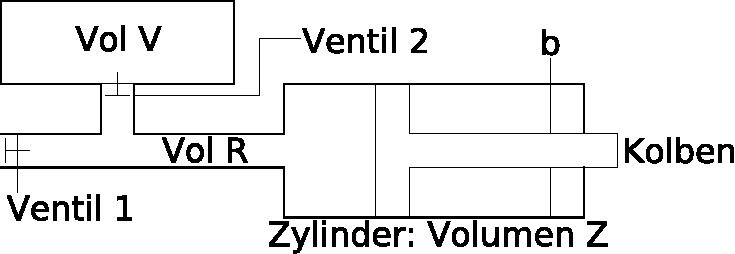
\includegraphics[width=0.8\textwidth]{include/evakuierungspumpe.pdf}
\begin{align*}
p_0: &\text{ Außendruck} \\
V: &\text{ zu evakuierendes Volumen} \\
R: &\text{ Restvolumen des Gestänges}
\end{align*}
\end{center}
%\end{minipage}

\begin{theorem}[Gasgesetz von Boyle-Mariotte]
\begin{align*}
p \cdot V = C \cdot m &&
\begin{aligned}
&p: \text{Druck} \\
&V: \text{Volumen} \\
&m: \text{Masse} \\
&C: \text{Boltzmann-Konstante}g
\end{aligned}
\end{align*}
\end{theorem}

\paragraph*{Funktionsweise}
\begin{itemize}
  \item Kolben in Stellung b; Ventil 1 offen; Ventil 2 geschlossen; d.h. Außenluft
  \item Kolben fährt nach a; Ventil 2 geschlossen; Ventil 2 geschlossen
  \item Kolben fährt nach b; Ventil 1 geschlossen; Ventil 2 offen; d.h. evakuiert V
\end{itemize}
Ergebnis: schrittweise Änderung des Drucks

\paragraph*{Modellierung}
\begin{enumerate}
	\item Kolbenhub (Stellung a)
	\begin{align*} \left.
		\begin{aligned}
			p_0 \cdot (V + R) &= C \cdot (m_v + m_r) \\
			\text{Kolben zu b} &= p_1 \cdot (V + R + Z)
		\end{aligned} \right\rangle
		p_1 = \frac{p_0 \cdot V + p_0 \cdot R}{V + R + Z}
	\end{align*}
	\item Kolbenschub
	\begin{align*}
	p_1 \cdot V + p_0 \cdot R &= p_2 \cdot (V + R + Z) && \text{Außendruck in R durch Öffnen des Ventils 1} \\
	p_2 &= \frac{p_1 \cdot V + p_0 \cdot R}{V + R + Z} \\
	&\vdots \\
	p_n &= \frac{p_{n-1} \cdot V + p_0 \cdot R}{V + R + Z} \\
	\end{align*}
\end{enumerate}
\begin{itemize} 
  \item Gibt es einen Grenzdruck $p_n \rightarrow p^*$?
  \item Auslegung von Z, R
\end{itemize}
Zahlenfolge $p_0, p_1, \ldots \rightarrow$\todo{unklar}

\end{example}

\begin{definition}[Zahlenfolge]
Eine Funktion $f: \mathbb N \rightarrow \mathbb N$ heißt reelle (Zahlen)folge.\\
Notation: $f_n$ oder $(f_n)_{n \in \mathbb N}$
\end{definition}

\begin{example}
\begin{enumerate}
	\item $a_n = n$: $a_1 = 1, a_2 = 2, \ldots$
	
\begin{tikzpicture}
	[uplabel/.style={above=4mm,anchor=center},
	 downlabel/.style={below=4mm,anchor=center}]
%\draw (0.5,0) -- (3.5,0)
% LH: scaling
\draw (0.5,0) -- (5,0)
(1,0) node (a1) {} node[uplabel] {$a_1$} node[downlabel] {1}
(2.75,0) node (a2) {} node[uplabel] {$a_2$} node[downlabel] {2}
(4.5,0) node (a3) {} node[uplabel] {$a_3$} node[downlabel] {3};
\foreach \n in {a1,a2,a3}
\draw (\n) ++(0,-0.1) -- ++(0,0.2);
\end{tikzpicture}\hspace{1cm}
\begin{tikzpicture}[line cap=round,line join=round,>=triangle 45,x=1.0cm,y=1.0cm]
\draw[color=white] (-1,0) -- (-0.5,0);
\draw[->,color=black] (-0.5,0) -- (2.5,0);
\foreach \x in {,1,2}
\draw[shift={(\x,0)},color=black] (0pt,2pt) -- (0pt,-2pt) node[below] {\footnotesize $\x$};
\draw[->,color=black] (0,-0.5) -- (0,2.5);
\foreach \y in {,1,2}
\draw[shift={(0,\y)},color=black] (2pt,0pt) -- (-2pt,0pt) node[left] {\footnotesize $\y$};
\draw[color=black] (0pt,-10pt) node[right] {\footnotesize $0$};
\clip(-0.5,-0.5) rectangle (2.5,2.5);
\fill [color=black] (1,1) circle (1.5pt);
\fill [color=black] (2,2) circle (1.5pt);
\end{tikzpicture}

	\item $a_n = \frac{1}{n}$: $a_1 = 1, a_2 = \frac{1}{2}, a_3 = \frac{1}{3}, \ldots$\label{ex:nullfolge}
	
	\begin{tikzpicture}
	[uplabel/.style={above=4mm,anchor=center},
	 downlabel/.style={below=4mm,anchor=center}]
% \draw (0.5,0) -- (3.5,0)
% LH: scaling
\draw (0.5,0) -- (5,0)
(1,0) node (n0) {}  node[downlabel] {0}
(4.5,0) node (a1) {} node[uplabel] {$a_1$} node[downlabel] {1}
(2.75,0) node (a2) {} node[uplabel] {$a_2$} node[downlabel] {$\frac{1}{2}$}
(2.17,0) node (a3) {} node[uplabel] {$a_3$} node[downlabel] {$\frac{1}{3}$};
\foreach \n in {n0, a1,a2,a3}
\draw (\n) ++(0,-0.1) -- ++(0,0.2);
\end{tikzpicture}\hspace{1cm}
\begin{tikzpicture}[line cap=round,line join=round,>=triangle 45,x=1.0cm,y=1.0cm]
\draw[color=white] (-1,0) -- (-0.5,0);
\draw[->,color=black] (-0.5,0) -- (3.5,0);
\foreach \x in {,1,2,3}
\draw[shift={(\x,0)},color=black] (0pt,2pt) -- (0pt,-2pt) node[below] {\footnotesize $\x$};
\draw[->,color=black] (0,-0.5) -- (0,1.5);
\foreach \y in {,1}
\draw[shift={(0,\y)},color=black] (2pt,0pt) -- (-2pt,0pt) node[left] {\footnotesize $\y$};
\draw[color=black] (0pt,-10pt) node[right] {\footnotesize $0$};
\clip(-0.5,-0.5) rectangle (3.5,1.5);
\fill [color=black] (1,1) circle (1.5pt);
\fill [color=black] (2,0.5) circle (1.5pt);
\fill [color=black] (3,0.33) circle (1.5pt);
\end{tikzpicture}

	\item $a_n = (-1)^n$: $a_1 = -1, a_2 = 1, \ldots$

	\begin{tikzpicture}
	[uplabel/.style={above=4mm,anchor=center},
	 downlabel/.style={below=4mm,anchor=center}]
%\draw (0.5,0) -- (3.5,0)
% LH: scaling
\draw (0.5,0) -- (5,0)
(2.75,0) node (n0) {}  node[downlabel] {0}
(1,0) node (a1) {} node[uplabel] {$a_1$}  node[downlabel] {-1}
(4.5,0) node (a2) {} node[uplabel] {$a_2$} node[downlabel] {1};
\foreach \n in {n0,a1,a2}
\draw (\n) ++(0,-0.1) -- ++(0,0.2);
\end{tikzpicture}\hspace{1cm}
\begin{tikzpicture}[line cap=round,line join=round,>=triangle 45,x=1.0cm,y=1.0cm]
\draw[color=white] (-1,0) -- (-0.5,0);
\draw[->,color=black] (-0.5,0) -- (4.5,0);
\foreach \x in {,1,2,3,4}
\draw[shift={(\x,0)},color=black] (0pt,2pt) -- (0pt,-2pt) node[below] {\footnotesize $\x$};
\draw[->,color=black] (0,-1.5) -- (0,1.5);
\foreach \y in {-1,1}
\draw[shift={(0,\y)},color=black] (2pt,0pt) -- (-2pt,0pt) node[left] {\footnotesize $\y$};
\draw[color=black] (0pt,-10pt) node[right] {\footnotesize $0$};
\clip(-0.5,-1.5) rectangle (4.5,1.5);
\fill [color=black] (1,-1) circle (1.5pt);
\fill [color=black] (2,1) circle (1.5pt);
\fill [color=black] (3,-1) circle (1.5pt);
\fill [color=black] (4,1) circle (1.5pt);
\end{tikzpicture}

\end{enumerate}
\end{example}

\paragraph*{Frage}
Streben die Folgen gegen ausgezeichnete Werte?
Im Beispiel \ref{ex:nullfolge} ist es der Null-Wert: $a_n \rightarrow 0$.\\
Zentrale Werkzeuge: Schranken und Monotonie

\begin{definition}[Beschränktheit]
Eine reelle Folge $(a_n)_{n \in \mathbb N}$ heißt nach oben beschränkt, falls ein reelles $L$ existiert mit
\begin{equation*} a_n \le L\end{equation*}
analog: nach unten beschränkt
\begin{equation*} a_n \ge L\end{equation*}
\end{definition}

\begin{example}
\begin{enumerate}
	\item untere Schranke $1$, keine obere Schranke
	\item untere Schranke $0$, obere Schranke $1$
	\item untere Schranke $-1$, obere Schranke $1$
\end{enumerate}
\end{example}

\begin{example}[Evakuierungspumpe, Fortsetzung]
Druckfolge $p_n$
\begin{itemize}
\item nach unten durch 0 beschränkt (da nur positive Terme)
\item nach oben durch $p_0$ beschränkt
\begin{align*}
p_1 &= p_0 \cdot \frac{V + R}{V + R + Z} < p_0 \\
p_2 &= \frac{p_1 \cdot V + p_0 \cdot R}{V + R + Z} < \frac{p_0 \cdot V + p_0 \cdot R}{V + R + Z} < p_0 \\
p_n &\text{ analog}
\end{align*}
\end{itemize}
\end{example}

\begin{definition}[Monotonie]
Eine reelle Folge heißt monoton wachsend, wenn $\forall n \in \mathbb N : a_n \le a_{n+1}$ und
streng monoton wachsend, wenn $a_n < a_{n+1}$. Analog: (streng) monoton fallend.
\end{definition}
Anschaulich: monoton wachsend + obere Schranke $\Rightarrow$ Grenzwert existiert $\equiv$ Supremumaxiom $\mathbb R$
\newpage
\lecture{2009-11-17}

\todo[inline]{könnte redundant zur vorheringen Vorlesung sein}
\begin{note}
 Falls eine Folge monoton und beschränkt ist, dann ist der Grenzwert die kleinste obere/untere Schranke. (Im Prinzip wäre man fertig, aber Folgen wie $a_n = \frac{(-1)^n}{n^2}$ würden nicht erfasst. $\leadsto$ Formalisierung erforderlich
\end{note}

\paragraph*{1. Schritt:} $\varepsilon$-Charakterisierung des Grenzwertes $\alpha$ \\
zu jedem $\varepsilon > 0$ ex. $n_\varepsilon$ mit $\alpha-\varepsilon < a_{n_\varepsilon}$
\paragraph*{2. Schritt:}
  \begin{equation*}
    \forall \varepsilon > 0\; \exists n_\varepsilon \;\forall n \geq n_\varepsilon: \;\left|a_n-\alpha\right| < \varepsilon
  \end{equation*}

\begin{definition}[Grenzwert]
  Eine Zahl $\alpha$ heißt Grenzwert (\emph{Limes}) einer Folge $a_n$, falls gilt:
  \begin{equation*}
    \forall \varepsilon > 0\; \exists n_\varepsilon \in \mathbb{N} \;\forall n \geq n_\varepsilon:\; \left| a_n - \alpha \right| < \varepsilon
  \end{equation*}
  Symbol: $\displaystyle\alpha = \liminfty{a_n}$\\
  Eine Folge heißt \emph{konvergent}, falls sie einen Grenzwert besitzt.
\end{definition}

\begin{note}[rekursiv definierte Folge]
  das $n$-te Folgenelement berechnet sich aus den Vorgängern
\end{note}

\begin{example}[rekursiv definierte Folge]
  Evakuierungspumpe: $p_n$ aus $p_{n-1}$ und $p_0$
\end{example}

\begin{note}[Grenzwert in drei Schritten]
  \begin{enumerate}
   \item beschränkt
   \item monoton
   \item Grenzwert berechnen durch Einsetzen $\displaystyle p^\ast = \liminfty{p_n}$
  \end{enumerate}
\end{note}

\begin{example}[Evakuierungspumpe]
  \[ p_n = \frac{p_{n-1}V+p_0R}{V+R+Z} \]
  \begin{enumerate}
    \item nach unten durch $0$ beschränkt
    \item monoton fallende Folge
    \item[$\Rightarrow$] es existiert ein Infimum $\inf p_n$ $\equals$ Grenzwert
    \item
      \begin{equation*}
        \liminfty{p_n} = \frac{\liminfty{p_{n-1}V}+p_0R}{V+R+Z} \Rightarrow
        p^\ast = \frac{p^\ast V+p_0R}{V+R+Z} = \frac{p_0R}{R+Z}
      \end{equation*}
  \end{enumerate}
\end{example}

\subsubsection*{Begriffe}

\emph{Konvergenz} -- es existiert ein Grenzwert\\
\emph{Divergenz} -- es existiert kein Grenzwert\\
\emph{Nullfolge} -- es existiert ein Grenzwert, dieser ist $0$

\subsubsection*{Rechenregeln für Nullfolgen}

\begin{note}
  konvergente Folge $a_n$ mit Grenzwert $\alpha \neq 0$ kann in Nullfolge transformiert werden: $b_n = a_n - \alpha$ ist Nullfolge
\end{note}

\begin{enumerate}
  \item $a_n, b_n$ Nullfolgen $\Rightarrow$ $a_n+b_n$ Nullfolge
  \item $a_n$ Nullfolge, $b_n$ beschränkt $\Rightarrow$ $a_n\cdot b_n$ Nullfolge
  \item $\left|b_n\right| < \left|a_n\right|$, $a_n$ Nullfolge  $\Rightarrow$ $b_n$ Nullfolge
\end{enumerate}

\begin{lemma}[Eindeutigkeit des Grenzwerts]
  Jede Folge $a_n$ hat höchstens einen Grenzwert.
\end{lemma}
\begin{proof}
  Angenommen, es existieren zwei Grenzwerte $\widehat a$ und $\overline a$, dann gilt nach Definition:
  \begin{align*}
    \left| a_n - \widehat a \right| &< \varepsilon \text{ für alle $n \geq N_1(\varepsilon)$} \\
    \left| a_n - \overline a \right| &< \varepsilon \text{ für alle $n \geq N_2(\varepsilon)$}
    \intertext{wähle $n \geq \max(N_1(\varepsilon),N_2(\varepsilon))$}
    \left| \widehat a - \overline a \right| &= \left| \widehat a - a_n + a_n - \overline a \right| \\
    & \leq \underbrace{\left| \widehat a - a_n \right|}_{< \varepsilon} + \underbrace{\left| a_n - \overline a \right|}_{< \varepsilon} \\
    & < \varepsilon + \varepsilon = 2\varepsilon
  \end{align*}
  $\Rightarrow \overline a = \widehat a$, da $\varepsilon$ beliebig klein aber $> 0$
\end{proof}

\begin{example}[Anwendungen]
\begin{enumerate}
  \item\label{ex:polynomlimes}
    \[
      \liminfty{x^n} = \begin{cases}
                          0 & \text{für $\left|x\right| < 1$ (Nullfolge)} \\
                          1 & \text{für $x=1$} \\
                          \infty & \text{für $x>1$} \\
                          \text{unbest.} & \text{für $x \leq -1$}
                       \end{cases}
    \]
  \item
    \begin{align*}
      a_n = \sqrt{n+1} - \sqrt n &\xrightarrow[n \rightarrow \infty]{} \infty - \infty = \text{?}\\
      &= \frac{(\sqrt{n+1}-\sqrt n)(\sqrt{n+1}+\sqrt n)}{\sqrt{n+1}+\sqrt n}\\
      &= \frac{n+1-n}{\sqrt{n+1}+\sqrt n}\\
      &= \frac 1 {\sqrt{n+1} + \sqrt n}\\
      &\xrightarrow[n \rightarrow \infty]{} 0
    \end{align*}
  \item geometrische Reihe
    \begin{equation*}
      s_n = 1 + x + \ldots + x^n = \begin{cases}
                                     \frac{1-x^{n+1}}{1-x} & \text{ für } x \neq 1 \\
                                     n + 1 & \text{ für } x = 1
                                   \end{cases}
    \end{equation*}
    aus Beispiel \ref{ex:polynomlimes}: nur konvergent für $\left| x \right| < 1$\\
    für $\left| x \right| < 1$:
    \begin{equation*}
      \liminfty{s_n} = \liminfty{\frac{1-x^{n+1}}{1-x}} = \frac{1-\displaystyle\liminfty{x^{n+1}}}{1-x} = \frac 1 {1-x}
    \end{equation*}
  \item harmonische Reihe\\
    Folge $s_n = \displaystyle 1 + \frac 1 2 + \frac 1 3 + \ldots + \frac 1 n$ ist divergent, denn
    \begin{align*}
      s_{2k+1} &= 1 + \frac 1 2 + \left( \frac 1 3 + \frac 1 4 \right) + \left( \frac 1 5 + \ldots \frac 1 8 \right) + \ldots + \left(\frac 1 {2^k+1} + \ldots + \frac 1 {2^{k+1}}\right) \\
      &\geq 1 + \frac 1 2 + 2 \cdot \frac 1 4 + 4 \cdot \frac 1 8 + \ldots + 2^k \cdot\frac 1 {2^{k+1}}\\
      &= \frac{k+3} 2 \\
      \Rightarrow \liminfty[k]{s_{2k+1}} &= \infty
    \end{align*}
    %
    \begin{note}
      Mantissenlänge (Zahldarstellung) und Taktzahl müssen so abgestimmt sein, dass ein unerfahrenere Nutzer in ca. 1 Tag Rechenzeit keine Konvergenz der harmonsichen Reihe erzielt (bisheriger Standard $R \ast 8$ nicht mehr ausreichend).
    \end{note}
  \item Eulersche Zahl $\euler = 2,71828\ldots$
    \begin{equation*}
      \euler := \sum\limits_{k=0}^\infty \left( \frac 1 {k!} \right) \rightarrow \text{ Grenzwert der Zahlenfolge}
    \end{equation*}
    \begin{enumerate}
      \item nach oben beschränkt
        \begin{align*}
          0 &\leq 1 + \frac 1 {1!} + \ldots + \frac 1 {n!} \\
          &\leq 1+1+\frac 1 2 + \ldots + \frac 1 {2^n}
        \end{align*}
      \item monoton wachsend
        \begin{equation*}
          b_{n+1} = 1 + \frac 1 {1!} + \ldots + \frac 1 {(n+1)!} = b_n + \frac 1 {(n+1)!} > b_n
        \end{equation*}
      \item[$\Rightarrow$] konvergent, Grenzwert $\leq 3$
    \end{enumerate}

\end{enumerate}

\end{example}
\lecture{2009-11-18}
%
\noindent weitere Darstellung von $\euler$:
\begin{equation*}
  \euler = \liminfty{\left(1+\frac 1 n\right)^n}\text{ (langsam konvergent)}
\end{equation*}
%
Weg zur Einführung der $\euler$-Funktion:
\begin{equation*}
  \text{z. z.} \forall x \in \mathbb{R}\; \left( 1 + \frac x n \right)^n \text{ konvergent}
\end{equation*}
Beweis siehe \cite[S. 32]{bornemann}

\begin{note}
  Bisher wurde in allen Definitionen und Erläuterungen Kenntnis eines Grenzwerts vorausgesetzt.\\
  Frage: Reichen Folgenelemente eventuell aus?\\
  Antwort: Cauchy'sche Folge
\end{note}

\begin{definition}[Cauchy-Folge]
  Die Folge $a_n$ heißt Cauchy-Folge, falls
  \[ \forall \varepsilon > 0\; \exists N(\varepsilon)\; \forall n,m \geq N\; |a_n-\underbrace{a_m}_{\text{Grenzwert } \alpha}| < \varepsilon \]
\end{definition}

\begin{proposition}
  $a_n$ konvergent $\Leftrightarrow$ $a_n$ ist Cauchyfolge
\end{proposition}

\begin{proof}
  \begin{itemize}
    \item[$(\Rightarrow)$]
      \begin{align*}
        \left| a_n - a_m \right| &= \left| a_n - \alpha + \alpha - a_m \right| \text{ (Grenzwert $\alpha$ existiert)}\\
        &\leq \left| a_n - \alpha\right| + \left| a_m - \alpha \right|
        \intertext{mit $n,m \geq N(\varepsilon)$}
        &=\varepsilon+\varepsilon = 2\varepsilon
      \end{align*}
      setze $\overline N (\varepsilon) = \displaystyle\frac{N(\varepsilon)} 2 \Rightarrow < 2$
    \item[$(\Leftarrow)$] 1780-1860\\
      Beweisidee:
      \begin{itemize}
        \item Beschränktheit der Cauchy-Folge
        \item $\frac 1 n, 1+\frac 1 n, 2+\frac 1 n, \frac 2 n, 1+\frac 2 n, 2+\frac 2 n, \ldots$
              \annotation{abwechselnd die Folgeglieder der Folgen $\frac 1 n$, $1+\frac 1 n$ und $2+\frac 1 n$}\\
              mehrere Kandidaten für Grenzwerte -- Häufungspunkte
              \annotation{Häufungspunkt wird ähnlich wie der Grenzwert definiert; jedoch brauchen nicht \emph{alle}, sondern nur \emph{unendlich viele} Folgeglieder in der $\varepsilon$-Umgebung liegen}
        \item Teilfolge, die gegen den Häufungspunkt konvergiert
        \item Bolzano-Weierstraß: Jede beschränkte Folge besitzt mindestens einen Häufungspunkt; eine konvergente Teilfolge ist auswählbar
        \item eindeutiger Grenzwert für Cauchy-Folge $\limsup$ bzw. $\liminf$
        \item Beweis siehe \cite[S. 29ff]{bornemann}
      \end{itemize}
  \end{itemize}
\end{proof}

\subsection{Stetige Funktionen}

Idee: Übertrage Grenzwerte im Definitionsbereich auf den Wertebereich\\
"`gutmütige"' Funktionen $f: I \to \mathbb{R}$, die einen Grenzprozess übertragen

\subsubsection*{formal}
\begin{equation*}
  \left.
  \begin{matrix}[rll]
    \text{linksseitiger Grenzwert} & x \longrightarrow a^+ & \displaystyle\lim_{x \rightarrow a^+} f(x) = c \\*[5mm]
    \text{rechtsseitiger Grenzwert} & x \longrightarrow a^- & \displaystyle\lim_{x \rightarrow a^-} f(x) = c
  \end{matrix}
  \right\}\Rightarrow \text{stetig}
\end{equation*}

\begin{definition}[Stetigkeit]
  $f: I \to \mathbb{R}$ heißt stetig in $x_0 \in I$, falls \begin{equation*} \lim_{x\rightarrow x_0} f(x) = f(x_0). \end{equation*} (alle denkbaren Folgen, die gegen $x_0$ konvergieren, sind zugelassen)

  $f$ heißt stetig, falls $f$ stetig in allen $x_0 \in I$ ist.
\end{definition}

\subsubsection*{anschaulich}
"`Zeichnen ohne den Stift abzusetzen"'

\begin{center}
\begin{tikzpicture}[]
 \draw[->,semithick] (-3,0) -- (3,0);
 \draw (-2,0.15) -- (-2,-0.15) node[below] {$a$};
 \draw (2,0.15) -- (2,-0.15) node[below] {$b$};
 \draw[domain=-2:2] plot [id=stetig_a, samples=50] function {0.1*(x**3)+1};
 \node at (0,1.7) {$f(x)$};
\end{tikzpicture}

\begin{tikzpicture}[]
 \draw[->,semithick] (-3,0) -- (3,0);
 \draw (-2,0.2) -- (-2,-0.2) node[below] {$a$};
 \draw (2,0.2) -- (2,-0.2) node[below] {$b$};
 \draw (-2,1) -- (-1.7,0.7) -- (-1.5,2.2) -- (-1.1,0.3) -- (0,1.3) -- (0.7,0.7) -- (1.2,3) -- (2,0.5);
 \node at (0,1.7) {$f(x)$};
 \node at (4,2) {"`Ecken erlaubt"'};
\end{tikzpicture}
\end{center}


\subsubsection*{Unstetigkeiten}

\begin{figure}[h]\centering

  \subfloat[Sprünge]{
  
\begin{tikzpicture}[]
 \draw[->,semithick] (-0.5,0) -- (3.5,0);
 \draw [)-|] (0,1) -- (1,1);
 \draw [)-|] (1,2) -- (2,2);
 \draw [)-|] (2,3) -- (3,3);
 %\node at (0,-1) {Sprünge};
\end{tikzpicture}
  }
  \subfloat[Lücken]{
\begin{tikzpicture}[]
 \draw[->,semithick] (-2.3,0) -- (2.3,0);
 \draw[domain=-2:0] plot [id=stetig_b1, samples=50] function {0.1*(x**3)+1};
 \draw[domain=0.5:2] plot [id=stetig_b2, samples=50] function {0.1*(x**3)+1.2};
 %\node at (0,-1) {Lücken};
\end{tikzpicture}
  }
  \subfloat[Polstellen]{
\begin{tikzpicture}[]
 \draw[->,semithick] (-2.3,0) -- (2.3,0);
 \draw (0,0.2) -- (0,-0.2) node[below] {$0$};
 \draw[domain=-2:-1.05] plot [id=stetig_c1, samples=30] function {(0.1*x)/((x+1)*(x-1))};
 \draw [ dashed](-1,1) -- (-1,-1);
 \draw[domain=-0.95:0.95] plot [id=stetig_c2, samples=30] function {(0.1*x)/((x+1)*(x-1))};
 \draw [ dashed](1,1) -- (1,-1);
 \draw[domain=1.05:2] plot [id=stetig_c3, samples=30] function {(0.1*x)/((x+1)*(x-1))};
 %\node at (0,-1) {Polstellen};
\end{tikzpicture}
  }
\end{figure}


\begin{theorem}[$\delta-\epsilon$-Charakterisierung analog zur Folgenkonvergenz]
  Für $f: I \to \mathbb{R}, x_0 \in I$ sind äquivalent:
  \begin{enumerate}
    \item $f$ stetig in $x_0$ (d. h. $\displaystyle\lim_{x\rightarrow x_0} f(x) = f(x_0)$)
    \item
      \begin{equation*}
        \forall \varepsilon > 0\; \exists \delta > 0\; \forall x \in I\; \left(
          \underbrace{\left| x-x_0\right| < \delta}_{\text{Definitionsbereich}} \Rightarrow
          \underbrace{\left| f(x)-f(x_0)\right| < \epsilon}_{\text{Wertebereich}}
        \right)
      \end{equation*}
  \end{enumerate}
\end{theorem}

\begin{center}
\begin{tikzpicture}[]
 \draw[->,semithick] (-0.5,0) -- (3,0) node[below]{x};
 \draw[->,semithick] (0,-0.5) -- (0,2.5) node[left]{y};
 \draw (1,0.2) -- (1,-0.2) node[below] {$x_0$};
 \draw (0.2,1) -- (-0.2,1) node[left] {$f(x_0)$};
 \draw [dashed] (0,1) -- (1,1) -- (1,0);
 \draw [dashed] (0,1.1) -- (1.55,1.1) -- (1.55,0);
 \draw [dashed] (0,0.9) -- (0.45,0.9) -- (0.45,0);
 \draw[domain=0:2.2] plot [id=stetig_d, samples=50] function {0.6*((x-1)**3)+1};
 \draw [|<->|] (2,1.1) -- (2,0.9) node [right] {\footnotesize $2\varepsilon$};
 \draw [|<->|] (1.55,-0.7) -- (0.45,-0.7) node[below right] {$\;\;2\sigma$};
\end{tikzpicture}
\end{center}



\begin{example}
  \begin{itemize}
    \item $\sin(\frac 1 x)$: unstetig
    \begin{center}
      \begin{tikzpicture}
        \draw[->,semithick] (-2.1,0) -- (2.1,0) node[below]{x};
        \draw[->,semithick] (0,-1.1) -- (0,1.1) node[left]{y};
        \draw[domain=-2:2] plot [id=sin_a, samples=400] function {sin(1/x)};
      \end{tikzpicture}
    \end{center}

    \item $x \cdot \sin(\frac 1 x)$: stetig ergänzbar an der Stelle 0, da Nullfolge $\cdot$ beschränkte Folge = Nullfolge (siehe Rechenregeln auf Seite \pageref{ssub:nullfolgen})
    \begin{center}
      \begin{tikzpicture}
        \draw[->,semithick] (-2.1,0) -- (2.1,0) node[below]{x};
        \draw[->,semithick] (0,-1.1) -- (0,1.1) node[left]{y};
        \draw[domain=-2:2] plot [id=sin_b, samples=400] function {x*sin(1/x)};
      \end{tikzpicture}
    \end{center}
  \end{itemize}
\end{example}

\subsubsection*{Rechenregeln stetiger Funktionen}

$f, g: I \to \mathbb{R}$ stetig

\begin{enumerate}
  \item $f\pm g$ stetig
  \item $\alpha \in \mathbb{R}$: $\alpha \cdot f$ stetig
  \item $f \cdot g$ stetig (Produkt der Funktionswerte)
  \item $g(x) \neq 0$: $\frac f g$ stetig
  \item Komposition/Hintereinanderausführung
    \begin{equation*}
      g(I) \subseteq I: \qquad (f \circ g)(x) = f(g(x)) \text{ stetig}
    \end{equation*}
\end{enumerate}
%
Beweise per $\delta-\epsilon$-Charakterisierung, siehe \cite{bornemann}

\subsubsection*{Folgerungen}

  \begin{enumerate}
    \item jedes Polynom $p(x) = a_0 + a_1 x + \ldots + a_n x^n$ ist stetig\\
      Argumentation:
      \begin{itemize}
        \item[] $f(x) = x$ stetig
        \item[$\Rightarrow$] $x^2, \ldots, x^k$ stetig
        \item[$\Rightarrow$] $a_k x^k, \ldots, a_1 x$ stetig
        \item[$\Rightarrow$] Summe stetig
      \end{itemize}
    \item jede rationale Funktion $r(x) = \frac{p(x)}{q(x)}$ ist bis auf Nullstellen im Nenner stetig
  \end{enumerate}

\subsubsection*{Eigenschaften stetiger Funktionen}

$f$ stetig auf dem Intervall $\left[a,b\right]$
  \begin{enumerate}
    \item $f$ ist beschränkt
      \begin{note}
        Zentral hierbei ist, dass es sich um ein abgeschlossenes Intervall handeln muss.

        Bsp.: $f(x) = \frac 1 x$, halboffenes Intervall $\left]0,1\right]$, $\displaystyle\lim_{x\rightarrow 0^+} = \infty$ $\Rightarrow$ Polstelle $\Rightarrow$ nicht beschränkt
      \end{note}
    \item $f$ nimmt Minimum/Maximum in diesem Intervall an (Extremwertsatz)
    \item falls $f(a) < 0$ und $f(b) > 0$, dann existiert ein $x^\ast$ mit $f(x^\ast) = 0$ (Zwischenwertsatz)
    
      (Beweis per Bisektionsverfahren, Intervallhalbierung)
  \end{enumerate}
\begin{center}
\begin{tikzpicture}
 \draw[->,semithick] (-0.2,0) -- (3,0) node[below]{x};
 \draw[->,semithick] (0,-2) -- (0,2) node[left]{y};
 \draw (1,0.2) -- (1,-0.2) node[below left] {$a$};
 \draw (2,0.2) -- (2,-0.2) node[below right] {$b$};
 \draw (-0.2,1) -- (0.2,1);
 \draw (-0.2,-1) -- (0.2,-1);
 \draw [dashed] (0,1) -- (2.5,1) node[right] {obere Schranke};
 \draw [dashed] (0,-1) -- (2.5,-1) node[right] {untere Schranke};
 \draw [dashed] (1,-1.5) -- (1,1.5);
 \draw [dashed] (2,-1.5) -- (2,1.5);
 \draw[domain=1:2] plot [id=sin_b, samples=400] function {sin(6*(x-0.5))};
\end{tikzpicture}
\end{center}


\newpage
\lecture{2009-11-24}
\section{Differenzierbarkeit}
\subsection{Ableitungsbegriff}

bisher: Stetige Funktion, die den Grenzprozess im Definitionsbereich auf den Wertebereich überträgt.\\
Frage: Ist es \emph{lokal} möglich eine Funktion \( f(x) \) genauer zu beschreiben? 

Wie sieht eine Funktion \( p(x) \) bzw. eine Gerade aus, die \( f(x) \) in \( x_0 \) möglichst gut beschreibt?
\[
p(x)=ax+b 
\]
\begin{center}
  \centering
\begin{tikzpicture}[scale=0.7, x=2cm, y=2cm]
	\draw[blue,domain=-2:2] plot ({\x},{(\x)^2}) node[above]{\( f(x)=x^2 \)};
	\draw[red,domain=-2:2.2] plot ({\x},{3}) node[anchor=mid west]{\( p_1 \)};
	\draw[red,domain=-2:0.5] plot ({\x},{(-\x)}) node[anchor=north west]{\( p_2 \)}; 
	\draw[green,domain=0:2.3] plot ({\x},{2*(\x)-1}) node[anchor=south west]{\( p \)};
\end{tikzpicture}
  \captionof{figure}{Die Geraden \( p_1(x) \) bzw. \( p_2(x) \) aus der Interpolation sind keine guten Repräsentanten. \(p(x)\) als Tangente in \(f(x_0)\) liegt hingegen gut.}
  \label{fig:Approximierung}
\end{center}
% LH: Polynominterpolation aus zwei Punkten -> Gerade
%\todo{JP:Welche Interpolation ist gemeint?}

\noindent Konstruktion der Geraden \( p(x) \), die die Funktion \( f(x) \) in der Nähe von \( x_0 \) gut beschreibt:

\[
	f:D\rightarrow\mathbb{R} \qquad D\subseteq\mathbb{R} \qquad x_0 \in D
\]

\begin{description}
	\item[1. Forderung] \( p(x_0)=f(x_0) \) 
	\begin{align*}
			p(x) &= ax+b \\
			f(x_0) &= ax_0+b \\
			\implies b &= f(x_0)-ax_0 \\
			\implies p(x) &= a(x-x_0)+f(x_0)
	\end{align*}
	\item[2. Forderung] \( d(x)=f(x)-p(x) \) soll in der Nähe von \( x_0 \) möglichst klein werden. Damit gilt \( d(x) = f(x) -f(x_0)-a(x-x_0) \)
	\item[1. Versuch] \( f(x) \) stetig  
	\[\lim_{x\rightarrow x_0} d(x)=\lim_{x\rightarrow x_0}(\underbrace{f(x)-f(x_0)}_{\rightarrow 0}-a\underbrace{(x-x_0)}_{\rightarrow 0})=0\]Dies ist nichts Neues, da die Information von \( a \) durch den Faktor \( (x-x_0) \) verdeckt wird.
	\item[2. Versuch] Forderung an Parameter \( a \in \mathbb{R} \)
	\[
		\lim_{x\rightarrow x_0}\left(\frac{f(x)-f(x_0)-a(x-x_0)}{x-x_0}\right)\stackrel{!}{=}0
	\]
	Die Division durch \( x-x_0 \) neutralisiert den Faktor \( a \).
\end{description}

\begin{definition}[Lineare Approximierbarkeit]
	\( f:D \to \mathbb{R} \) heißt linear approximierbar in \( x_0 \in D \), falls ein \( a \in \mathbb{R} \) existiert mit
        \[ \lim_{x\rightarrow x_0}\left(\frac{f(x)-f(x_0)-a(x-x_0)}{x-x_0}\right)=0 \]
\end{definition}

\begin{note}
  \begin{itemize}
    \item Die Herleitung ist auch auf \( \mathbb{R}^n \) übertragbar.
    \item \( f \) heißt auch \emph{differenzierbar} in \( x_0 \)
  \end{itemize}
\end{note}

\begin{example} 
\[
f(x)=x^2 \qquad x_0=1 \implies f(x_0)=1
\]
\begin{align*}
  \frac{f(x)-f(x_0)-a(x-x_0)}{x-x_0} &= \frac{x^2-1-a(x-1)}{x-1} \\
  &= \frac{(x-1)(x+1)-a(x-1)}{x-1} \\
  &= x+1-a
\intertext{nach Def. der linearen Approximierbarkeit -- Grenzwertbildung}
  0 &= \lim_{x \rightarrow x_0} \left(x+1-a\right) \\
  &= \left(x+1-a\right) \\
  \implies a &= 2
\end{align*}
\end{example}
	
\begin{definition}[1. Ableitung]
	\( f:D\rightarrow \mathbb{R} \) heißt differenzierbar in \( x_0 \in D \) falls obiger Grenzwert existiert.
\end{definition}
\begin{note}
  Die durch \( f \) und \( x_0 \) festgelegte Zahl \( a \) heißt 1. Ableitung von \( f \) in \( x_0 \).


\begin{equation*}
	f'(x_0) = \dot{f}(x_0) = \lim_{x\rightarrow x_0}\left(\frac{f(x)-f(x_0)}{x-x_0}\right) =:\text{ "`Differentialquotient"'}
\end{equation*}

\end{note}

\begin{note}
  Graph von \( p(x) \) lässt sich deuten als Tangente an \( f \) im Punkt \( x_0 \) (siehe \ref{fig:Approximierung})
\end{note}

\begin{example}[Einfache Differentiationsgleichung \( f(x)=x^n \)]
\begin{align*}
	\lim_{x \rightarrow x_0} \left(\frac{f(x)-f(x_0)}{x-x_0} \right)
	&= \lim_{x \rightarrow x_0} \left(\frac{x^n-x_0^n}{x-x_0}\right) \\
	&= \lim_{x \rightarrow x_0} \left(\sum_{k=0}^{n-1}x_0^kx^{n-1-k}\right) \\
	&= \sum_{k=0}^{n-1}x_0^kx_0^{n-1-k} \\
	&= \sum_{k=0}^{n-1}x_0^kx_0^{n-1} = nx^{n-1} 
\end{align*}

\[
	f(x)=x^n \quad \text{allg.: } \forall x_0 \in \mathbb{R} \quad f'(x)=nx^{n-1}
\]
\end{example}
\noindent Idee von Leibniz: approximiere die Steigung der Tangente in \( x_0 \) durch Sekanten

\[	\text{Grenzprozess } x \rightarrow x_0 \]
\[	\Leftrightarrow \]
\[	\text{Sekantensteigung } \equals \text{ Tangentensteigung} \]
\[	\Leftrightarrow \]
\[	\text{Differentialquotient} \leftrightarrow \text{Differenzenquotient} \]
\[	\frac{f(x)-f(x_0)}{x-x_0} \rightarrow \frac{\Delta f}{\Delta x}\]

\subsubsection*{Bezeichnungen}
\begin{equation*}
	f'(x_0) \qquad \frac{\diff f}{\diff x}(x_0) \qquad \left.\frac{\diff f}{\diff x}\right|_{x=x_0}
\end{equation*}
%
setze \( x = x_0 \):
\begin{equation*}
  \lim_{x \rightarrow x_0}\left(\frac{f(x)-f(x_0)}{x-x_0}\right) = \lim_{h \rightarrow 0}\left(\frac{f(x_0+h)-f(x_0)}{h}\right)
\end{equation*}
% LH: man geht von x->x0 über zu h->0
%\todo{JP:Zusammenhang ist mir unklar.}

\subsection{Rechenregeln für Funktionen}
\label{sec:rechenregeln_f_funktionen}

\begin{theorem}[Differenzierbarkeit $\Rightarrow$ Stetigkeit]
  Jede in \( x_0 \in D \) differenzierbare Funktion \( f \) ist stetig in \( x_0\).
\end{theorem}
\begin{proof}
  \[ \lim_{x \rightarrow x_0} (f(x)-f(x_0)-\underbrace{f'(x_0)}_{\in \mathbb{R} \text{ und fest} }\underbrace{(x-x_0)}_{\longrightarrow 0}) = 0 \]
\end{proof}

\begin{theorem}[Stetigkeit $\not\Rightarrow$ Differenzierbarkeit]
  Nicht jede stetige Funktion ist differenzierbar.
\end{theorem}

\begin{example}
\[	f(x)=|x| \qquad \text{ in } x_0=0 \text{ hat die Funktion eine "`Spitze"' } \]
\[	\text{formal: } \lim_{h \rightarrow 0}\frac{f(x_0+h)-f(x_0)}{h} = \lim_{h \rightarrow 0}\frac{|h|}{h}  \]
  Fallunterscheidung:
  \begin{itemize}
    \item von links \[\displaystyle\lim_{h \rightarrow 0^-}\frac{|h|}{h} = -1\]
    \item von rechts \[\displaystyle\lim_{h \rightarrow 0^+}\frac{|h|}{h} = 1\]
  \end{itemize}

\end{example}

\begin{center}
  \begin{tikzpicture}[scale=0.7, x=2cm, y=2cm]
    \draw[->,color=black] (-2.5,0) -- (2.5,0);
    \foreach \x in {-2,-1,1,2}
    \draw[semithick,shift={(\x,0)},color=black] (0pt,2pt) -- (0pt,-2pt) node[below] {\footnotesize $\x$};
    \draw[->,color=black] (0,-0.5) -- (0,2.5);
    \foreach \y in {,1,2}
    \draw[semithick,shift={(0,\y)},color=black] (2pt,0pt) -- (-2pt,0pt) node[left] {\footnotesize $\y$};
    \draw[color=black] (0pt,-10pt) node[right] {\footnotesize $0$};
    \draw[blue,samples=200,domain=-2:2] plot ({\x},{(abs(\x))}) node[above]{\( f(x)=|x|\)};
  \end{tikzpicture}
  \captionof{figure}{Betragsfunktion \( f(x)=|x| \)}
  \label{fig:Betragsfunktion}
\end{center}

\subsubsection*{Einfache differenzierbare Funktionen}
\begin{enumerate}
	\item \( f(x)=c \text{ (Konstante)} \implies f'(x)=0 \)
	\item \( f(x)=ax+b \implies f'(x)=a \)
	\item \(f(x)=x^2 \implies f'(x)=2x \)\newline
		  \(f(x)=x^n \implies f'(x)=nx^{n-1} \)
	\item \( f(x)=\sqrt{x} \qquad x>0 \implies f'(x)=\frac{1}{2\sqrt{x}} \)
	 \begin{proof}
	   \[ x_0>0 \qquad \lim_{x \rightarrow x_0}\frac{\sqrt{x}-\sqrt{x_0}}{x-x_0} =
            \lim_{x \rightarrow x_0}\frac{1}{\sqrt{x}+\sqrt{x_0}}=\frac{1}{2\sqrt{x_0}} \]
	 \end{proof}

\end{enumerate}


% Graph der Wurzelfunktion mit der Bemerkung das x_0=0 nicht diffbar ist
\begin{center}
\begin{tikzpicture}[scale=0.7, x=2cm, y=2cm]
	\draw[->,semithick,color=black] (-0.5,0) -- (3.5,0);
	\foreach \x in {,1,2,3}
	\draw[shift={(\x,0)},color=black] (0pt,2pt) -- (0pt,-2pt) node[below] {\footnotesize $\x$};
	
	\draw[->,semithick,color=black] (0,-0.5) -- (0,2);
	\foreach \y in {,1}
	\draw[shift={(0,\y)},color=black] (2pt,0pt) -- (-2pt,0pt) node[left] {\footnotesize $\y$};
	\draw[blue,domain=0:3,samples=200] plot ({\x},{(sqrt(\x))}) node[above]{\( f(x)=\sqrt{x}\)};
\end{tikzpicture}
\captionof{figure}{Wurzelfunktion: an der Stelle \( x_0=0 \) nicht differenzierbar}
\label{Wurzelfunktion}
\end{center}


\subsubsection*{Rechenregeln} % (fold)
\label{sub:rechenregeln}

\( f,g:D\rightarrow\mathbb{R} \) für alle \( x \in D \) differenzierbar

\begin{enumerate}
	\item \( f \pm g \) differenzierbar mit \( (f(x)\pm g(x))'=f'(x)\pm g'(x) \)
	\item \( c \cdot f \) differenzierbar, \( c \in \mathbb{R} \), \( (c \cdot f(x))'=c\cdot f'(x) \)
	\item Produktregel \( (f(x) \cdot g(x))' = f'(x) \cdot g(x)+f(x) \cdot g'(x) \)
	\item Quotientenregel, \( g(x) \neq 0 \), \( \left(\cfrac{f(x)}{g(x)}\right)'=\cfrac{f'(x)\cdot g(x)-f(x)\cdot g'(x)}{g(x)^2} \) \\
          speziell: \( \left(\cfrac{1}{g(x)}\right)'=-\cfrac{g'(x)}{g(x)^2} \)
\end{enumerate}

\begin{proof}
  \begin{enumerate}
    \item trivial
    \item trivial
    \item Herleitung:
      \begin{align*}
        (f\cdot g)'(x) &= \lim_{h \rightarrow 0}\frac{(f \cdot g)(x_0+h)-(f \cdot g)(x_0)}{h}\\
        &= \lim_{h \rightarrow 0}\frac{f(x_0+h) g(x_0+h) - f(x_0)  g(x_0)} h \\
        &= \lim_{h \rightarrow 0}\frac{f(x_0+h) g(x_0+h) \color{blue}- f(x_0) g(x_0+h)\color{black} - f(x_0)  g(x_0) \color{blue}+ f(x_0)  g(x_0+h)\color{black}} h\\
        &= \lim_{h \rightarrow 0}\frac{(f(x_0+h) - f(x_0))\cdot g(x_0+h) + (g(x_0+h) - g(x_0)) \cdot f(x_0) } h\\
        &= \lim_{h \rightarrow 0}\frac{f(x_0+h) - f(x_0)} h \cdot g(x_0+h) + \frac{g(x_0+h) - g(x_0)} h \cdot f(x_0)\\
        &= f'(x_0) \cdot g(x_0) + g'(x_0) \cdot f(x_0)
      \end{align*}
    \item \todo{Herleitung fehlt}
  \end{enumerate}
\end{proof}

% subsubsection rechenregeln (end)
% subsection rechenregeln_für_funktionen (end)
\lecture{2009-11-25}

\subsubsection*{Folgerungen}

\begin{enumerate}
	\item Polynome sind überall differenzierbar \\
	\begin{align*}
		p(x) &= a_0 + a_1 x + \dots + a_n x^n \\
		\Rightarrow p'(x) &= a_1 + 2 a_2 x + 3 a_3 x^2 + \dots + n a_n x^{n-1}
	\end{align*}
	\begin{note}Berechnung von Polynom und Ableitung gleichzeitig über \emph{vernetztes Hornerschema} möglich\end{note}
	\item rationale Funktionen sind bis auf Polstellen differenzierbar\annotation{bei rationalen Funktionen können auch Definitionslücken auftreten, die aber stetig fortsetzbar sind}
	\begin{align*}
		r(x) &= \frac{p(x)}{q(x)} \\
		\left( \frac{1}{x} \right)' &= -\frac{1}{x^2} \\
		\left( \frac{1}{x^n} \right)' &= -\frac{n}{x^{n+1}} \hspace{10px} (x \neq 0)
	\end{align*}
	Herleitung (siehe auch Beweis der Quotientenregel auf Seite \pageref{proof:quotregel}):
	\begin{align*}
		\left( \frac{1}{x} \right)' &= \lim\limits_{h \rightarrow 0} \frac{\frac{1}{x_0+h} - \frac{1}{x_0}}{h} \\
		&= \lim\limits_{h \rightarrow 0} \frac{1}{h} \left( \frac{x_0 - x_0 - h}{x_0 (x_0+h)} \right) \\
		&= - \lim\limits_{h \rightarrow 0} \frac{1}{x_0 (x_0 + h)} \\
		&= -\frac{1}{x^2}
	\end{align*}
\end{enumerate}

\subsubsection*{Trigonometrische Funktionen}
\begin{enumerate}
	\item $ (\sin x)' = \cos x $
	\item $ (\cos x)' = - \sin x $
	\item $ (\tan x)' = \cfrac{1}{\cos^2 x} $
\end{enumerate}

\begin{proof}
  \begin{enumerate}
   \item 
\begin{align*}
 	(\sin x)' &= \lim_{h \rightarrow 0}\frac{\sin (x + h) - \sin x}{h}
\intertext{Additionstheorem:}
	\sin(x+y) &= \sin x \cos y + \sin y \cos x
\intertext{damit}
	(\sin x)' &= \lim_{h \rightarrow 0}\frac{\sin x \cos h + \sin h \cos x - \sin x}{h} \\
	&= \lim_{h \rightarrow 0}\sin x \underbrace{\frac{\cos h - 1}{h}}_{\xrightarrow{h \rightarrow 0} 0 \ast} + \cos x \underbrace{\frac{\sin h}{h}}_{\xrightarrow{h \rightarrow 0} 1} \\
	&= \cos x
\end{align*}
%
letzter Schritt zu zeigen über:
\begin{itemize}
	\item Dreiecke
	\item Potenzreihen
		\begin{align*}
			\cos x &= 1 - \frac{x^2}{2!} + \frac{x^4}{4!} \dots \\
			\sin x &= x - \frac{x^3}{3!} + \frac{x^5}{5!} \dots
		\end{align*}
\end{itemize}

    \item Additionstheorem $\cos (x + h)$
    \item $ \tan x = \cfrac{\sin x}{\cos x}$ $\implies$ Quotientenregel $\implies$  $1+\tan^2 x = \frac 1 {\cos^2 x}$%
      \annotation{identisch wegen $\sin^2 x +\cos^2 x = 1$ ("`trigonometrischer Pythagoras"')}
  \end{enumerate}
\end{proof}


\subsubsection*{Kettenregel (Chain Rule)}
Anwendung bei Neuronalen Netzen: Lernregeln $\equals$ Kettenregeln \\
$f, g$ seien differenzierbar \\
Komposition/Hintereinanderausführung
\begin{equation*}
	(f \circ g)(x) = f(g(x))
\end{equation*}
\begin{equation*}
	g: I \rightarrow \mathbb{R}, f: D \rightarrow \mathbb{R}, g(I) \in D
\end{equation*}
\begin{equation*}
	(f \circ g)' (x_0) = \underbrace{f'(g(x_0))}_{\text{äußere Ableitung}} \cdot \underbrace{g'(x_0)}_{\text{innere Ableitung}}
\end{equation*}
Kurzform\annotation{Kürzen von $\diff g$ ist \emph{keine} gültige Operation}:
\begin{equation*}
	\frac{\diff (f \circ g)}{\diff x} = \frac{\diff f}{\diff g} \frac{\diff g}{\diff x}
\end{equation*}
Beweisidee (nicht sauber, da der Nenner eventuell $0$ wird):
\begin{equation*}
  \begin{array}{rcccc}\displaystyle
    \frac{(f \circ g)(x_0 + h) - (f \circ g)(x_0)}{h} &=& \multicolumn{3}{l}{\displaystyle\frac{f(g(x_0 + h)) - f(g(x_0))}{h}} \vspace{.5cm}\\
    &=& \displaystyle\frac{f(g(x_0 + h)) - f(g(x_0))}{\textcolor{blue}{g(x_0 + h) - g(x_0)}} & \cdot & \displaystyle\frac{\textcolor{blue}{g(x_0 + h) - g(x_0)}}{h} \vspace{.1cm}\\
    & & \downarrow & & \downarrow\vspace{.1cm} \\
    \multicolumn{2}{r}{\xrightarrow{h \rightarrow 0}} & f'(g)(x_0) & \cdot & g'(x_0)
  \end{array}
\end{equation*}

\begin{example}
	Kubische Hermite-Polynome
	\begin{equation*}
		p(t):\; t = \frac{x-x_0}{h}
	\end{equation*}
	
	\begin{enumerate}
		\item
		\begin{align*}
			h(x) &= (x^2 + 3x + 1)^4\\
			f(x) &= x^4 &\text{äußere Funktion} \\
			g(x) &= x^2 + 3x + 1 &\text{innere Funktion} \\
			\\
			h'(x) &= \underbrace{4 (x^2 + 3x + 1)^3}_{\parbox{23mm}{\centering\scriptsize \text{äußere Ableitung} f'(g)}}\;\;\cdot\!\! \underbrace{(2x + 3)}_{\parbox{23mm}{\centering\scriptsize \text{innere Ableitung} g'(x)}}
		\end{align*}
		
		\item
		\begin{align*}
			h(x) &= \sqrt{x^3 + \sqrt{x^5}} \\
			f(x) &= \sqrt{x} & \text{äußere Funktion}\\
			g(x) &= x^3 + \sqrt{x^5} & \text{1. innere Funktion} \\
			k(x) &= \sqrt{x^5} & \text{2. innere Funktion}
		\end{align*}
		
		\begin{align*}
			h'(x) &= \frac{\mathrm dh}{\mathrm dx} = 
			\frac{\mathrm df}{\mathrm dg}\frac{\mathrm dg}{\mathrm dx} =
			\frac{1}{2\sqrt{g(x)}} \left( 3x^2 + \frac{\mathrm d}{\mathrm dx} \left( \sqrt(x^5) \right)\right) \\
			\\
			\frac{\mathrm dh}{\mathrm dx} \sqrt{x^5} &= \underbrace{\frac{1}{2\sqrt{x^5}}}_{\frac{1}{2k(x)}} 5x^4
		\end{align*}
	\end{enumerate}
\end{example}

\begin{definition}[Höhere Ableitungen]
	\begin{align*}
		f&: D \rightarrow R \text{ beliebig oft differenzierbar} \\
		f^{(0)}(x) &:= f(x) \\
		(k \geq 0) \hspace{10px} f^{(k+1)}(x) &:= \frac{\mathrm d}{\mathrm dx} \left( f^{(k)}(x) \right)
	\end{align*}
\end{definition}
	
\begin{equation*}
\begin{array}{llll}
	& f \\
	\text{1. Ableitung} & f' &= \frac{\mathrm d}{\mathrm dx}f & \text{Geschwindigkeit} \\
	\text{2. Ableitung} & f'' &= \frac{\mathrm d}{\mathrm dx}f' & \text{Beschleunigung} \\
	\text{3. Ableitung} & f''' &= \frac{\mathrm d}{\mathrm dx}f'' & \leadsto \text{ Autobahnausfahrt}
\end{array}
\end{equation*}

\subsection{Schwingungsgleichung -- Gewöhnliche Differentialgleichung}
(siehe auch \cite[Kap. 8]{bornemann})

% LH: erstmal durch subsubsection ersetzt
%\todo{Wenn keine weiteren Items in der nächsten Vorlesung kommen itemize wieder ausbauen}
%\begin{itemize}
%	\item Schwingung einer Feder
	
\subsubsection*{Schwingung einer Feder}
	\begin{center}
		\begin{tikzpicture}[scale=1, x=1cm, y=1cm]
			\draw (0.3,1) -- (5,1);
			\draw (1,1) -- (1.5, 1.5);
			\draw (2,1) -- (2.5, 1.5);
			\draw (3,1) -- (3.5, 1.5);
			\draw (4,1) -- (4.5, 1.5);

			\draw[o-] (2.5, 1) -- (2.5, 0.5);
			\draw[decorate,decoration={coil,segment length=4pt}] (2.5, 0.5) -- (2.5, -2);
			\draw (2.5, -2) -- (2.5, -2.5);

			\draw (2, -2.5) rectangle (3, -3.5);

			\draw (5.5, 1) rectangle (6, -4.5);

			\draw[o->] (3, -3) -- (5.5, -3);

			\draw (5.5, -3) -- (6, -3) node [right] {$s = 0$};

			\draw[->] (6.5, -2.5) -- (6.5, -1.5);
			\draw[->] (6.5, -3.5) -- (6.5, -4.5);

			\draw (5.5, -4.5) node [below] {Messskala};
		\end{tikzpicture}
	\end{center}
	Anfangsauslenkung führt zu einer Schwingung (ohne Schwerkraft) \\
	Weg-Zeit-Diagramm
	\begin{itemize}
		\item Eichung: $t = 0$
		\item Ruhelage $ s = 0$ 
		\item Anfangsgeschwindigkeit $v \neq 0$
		\item Weg $s(t)$
		\item Geschwindigkeit $\dot s(t)$
		\item Beschleunigung $\ddot s(t)$
	\end{itemize}
	Kräftegleichgewicht:
	\begin{itemize}
		\item Newton-Kraft: $k_1 = m \ddot s(t)$
		\item Federgesetz: $k_2$ entspricht Auslenkung $k_2 = D s(t)$
	\end{itemize}
	%
	Prinzip D'Alembert: "`Summe aller Kräfte"' = 0
	\begin{align*}
		k_1 + k_2 &= 0 \\
		m \ddot s + D s &= 0 \\
		\Rightarrow \ddot s(t) + \frac{D}{m} s(t) &= 0
	\end{align*}
	
	\begin{equation*}
		k = \sqrt{\frac{D}{m}} \text{ Frequenz: $s^{-1}$}
	\end{equation*}
	%
	Schwingungsgleichung:
	\begin{equation*}
		\mathbf{\ddot s(t) + k^2 s(t) = 0}
	\end{equation*}
	% LH: andere Art der Hervorhebung ausgewählt
	%\todo{Kasten um Schwingungsgleichung und DGL}
	%
	Aufgabe: Suche $s(t)$, welches obige Gleichung unter den Anfangsbedingungen $s(0) = 0$, $ \dot s(0) = v_0$ erfüllt.
	\begin{definition}
	Eine Verknüpfung einer unbekannter Funktion $s(t)$ mit ihren Ableitungen heißt \emph{gewöhnliche Differentialgleichung}.
	\end{definition}
	
	\begin{equation*}
		\left.
		\begin{matrix}[rl]
			\ddot s + k^2 s = 0 & \text{2. Ableitung} \\
			s(0) = 0, \dot s(0) = v_0 & \text{lineares System}
		\end{matrix}
		\right\}
		\text{lineare DGL 2. Ordnung}
	\end{equation*}
	%
	allgemein:
	\begin{align*}
		\dot y(t) &= f(t, y) \\
		y(t_0) &= y_0
	\end{align*}
	\begin{equation*}
		\begin{matrix}
			f: &I& \hspace{-10px}\times \mathbb{R}^{(n)} \to \mathbb{R}^{(n)} \\
			& \downarrow & \\
			& t &
		\end{matrix}
	\end{equation*}
%\end{itemize}
\lecture{2009-12-01}

\paragraph{Übersicht}

\begin{itemize}
	\item $\ddot s + k^2s = 0$ ist eine Differentialgleichung (Dgl.) und "`verknüpft"' Funktionswerte und Ableitungen der unbekannten (gesuchten) Funktion $s(t)$.
	\item Da nur eine unabhängige Variable (hier die Zeit $t$) existiert handelt es sich um eine gewöhnliche Differentialgleichung (ODE, ordinary differential equation).
	\item Da nur die Anfangswerte $s(0)$ und $\dot s(0)$ gegeben sind ist es ein Anfangswerteproblem (AWP) oder englisch initial value problem (IVP).
	\begin{note}
		Existieren mehrere unabhängige Variablen ($x, y, z \in \mathbb{R}^3, t \in \mathbb{R}^+$) handelt es sich um eine partielle Differentialgleichung (partial diffenrential equation, PDE).
		\begin{example}
			\begin{itemize}
				\item Wärmeleitung: $u_t = \alpha^2 u_{xx}$\annotation{Zur Notation: $u_{xx} \equals \frac{\partial^2}{\partial x^2}u(x,t)$, $u_t$ entsprechend.}
				\item Wellengleichung: $u_{tt} = c^2 u_{xx}$
				\item Laplace-Gleichung: $\Delta u = u_{xx} + u_{yy} + u_{zz} = f(t, u)$
			\end{itemize}
		\end{example}
	\end{note}
	\item $\ddot s + k^2s = 0$ ist eine Dgl. zweiter Ordnung, da die höchste enthaltene Ableitung zweiter Ordnung ist.
\end{itemize}

\paragraph{Fragen}
\begin{enumerate}
	\item Wie berechne ich \underline{eine} Lösung?
	\item Wie berechne ich \underline{alle} Lösungen?
	\item Definitionsbereich einer Lösung?
\end{enumerate}
Obige Fragen sind in der "`ODE-Welt"' beantwortbar, erfordern in der "`PDE"'-Welt hingegen 1 - 20 Jahre zur Lösung.

\paragraph{Spezielle Herangehensweise:} $\ddot s(t) + k^2s(t) = 0 \rightarrow$ Technik des intelligenten Ratens!

\subparagraph{Für $k = 1$}
\begin{align*}
	& \ddot s + s = 0 \\
	\rightarrow &\text{ geraten: z. B. $s_1(t) = \sin(t)$, $s_2(t) = \cos(t)$}\\
	\Rightarrow &s_1(t) = \sin kt \\
	\Rightarrow &s_2(t) = \cos kt \\
	& \ddot s(t) + k^2s(t) = 0 \text { ist linear } \leadsto \text{ Überlagern ($Ax = 0$, $Ax = b$)} \\
	\Rightarrow &s(t) = c_1 \sin kt + c_2 \cos kt \text{ allgemeine Lösung, $c_1, c_2 \in \mathbb{R}$} \\
	\intertext{Parameter $c_1$, $c_2$ an Anfagswerte adaptieren.}
	&\left. \begin{aligned}
		\rightarrow s(0) &= 0 \Rightarrow c_2 = 0 \\
		\rightarrow \dot s(0) &= v_0 \Rightarrow c_1k = v_0 \Rightarrow c_1 = \frac{v_0}{k}
	\end{aligned} \right\} \text {AWT $s(t) = \frac{v_0}{k}$ sinkt} \\
	&\left. \begin{aligned}
		s(t) &= c_1 \sin kt \\
		\dot s(t) &= c_1k \cos kt \\
		\ddot s(t) &= c_1k^2 \sin kt
	\end{aligned} \right\}\ddot s(t) + k^2s(t) = 0
\end{align*}

\subsubsection{Schwingungsgleichung in $\mathbb{C}$: $\ddot s + k^2s = 0$}

\paragraph{Euler-Formel: $\euler^{i\varphi} = \cos \varphi + i \sin \varphi$}
\begin{align*}
	\frac{d}{d\varphi}\euler^{i\varphi} &= \frac{d}{d\varphi}(\cos \varphi + i \sin \varphi) = -\sin \varphi + i\cos \varphi \\
	\frac{d}{d\varphi}\euler^{ik\varphi} &= \frac{d}{d\varphi}(\cos k\varphi + i \sin k\varphi) =\\ &= -k\sin k\varphi + ik\cos k\varphi = ik(\cos k\varphi + i\sin k\varphi) = ik\euler^{ik\varphi} \\
	\frac{d^2}{d\varphi^2}(\euler^{ik\varphi} &= i^2k^2\euler^{ik\varphi} = -k^2 \euler^{ik\varphi} \\
	S(t) &= C_1s_1(t) + C_2s_2(t) = C_1\euler{ikt} + C_2\euler{-ikt} \\&\text{ mit $C_1 = c_1 + ic_2$ und $C_2 = d_1 + id_2$}
\end{align*}
Es gilt: $s(t) = Re(S(t))$ (Umrechnung in der Übung)

\subsection{Anwendung der Differentiation}
\begin{wrapfigure}{r}{0.45\textwidth}
 	\begin{center}
		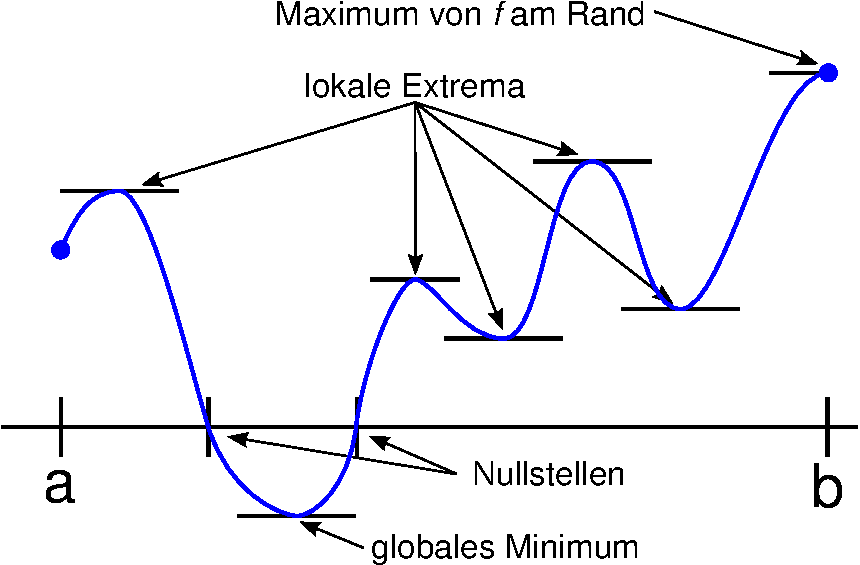
\includegraphics[width=0.45\textwidth]{include/20091201-1.pdf}
	\end{center}
\end{wrapfigure}
Ziel: Kurvendiskussion von $f: I \rightarrow \mathbb{R}$ (differenzierbar)
\begin{definition}
	Lokales Maximum von $f$ in $x_0$ (im Inneren)
	\begin{equation*}
		f(x) \leq f(x_0) \quad |x - x_0| < \delta,\;\delta>0\text{ geg.}
	\end{equation*}
	Im Inneren: waagrechte Tangente $f(x_0) = 0$ charakterisiert lokales Extremum (notwendige Bedingung).
\end{definition}
\begin{note}
	$f(x) = x^3 \leadsto f'(0) = 0$ aner kein lokales Extremum
\end{note}

\subsubsection{Satz von Rolle}
\begin{wrapfigure}{r}{0.4\textwidth}
 	\begin{center}
		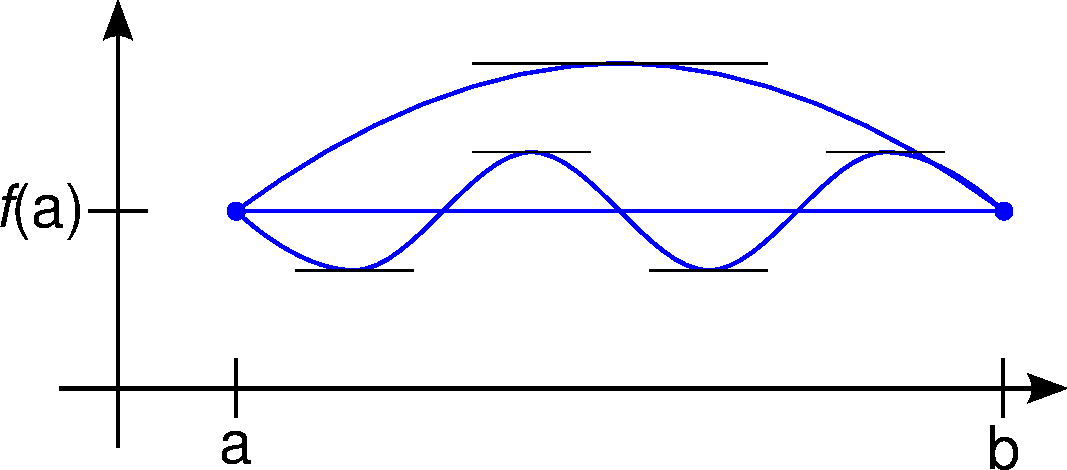
\includegraphics[width=0.4\textwidth]{include/20091201-2.pdf}
	\end{center}
\end{wrapfigure}
Gegeben: $f:[a, b] \rightarrow \mathbb{R}$ sei differenzierbar und es gilt $f(a) = f(b)$.
Es gilt: Es existiert ein $x_0$ mit $a < x_0 < b : f'(x_0) = 0$ oder $f$ ist konstant. Umgangssprachlich: "`$f$ ist entweder konstant oder besitzt ein Extremum."'
Uminterpretation: Sekantensteigung an Intervallenden: Es existiert ein $x_0$ mit gleicher Tangentensteigung.

\subsubsection{1. Mittelwertsatz der Integralrechnung (1. MWS)}
\begin{wrapfigure}{l}{0.4\textwidth}
 	\begin{center}
		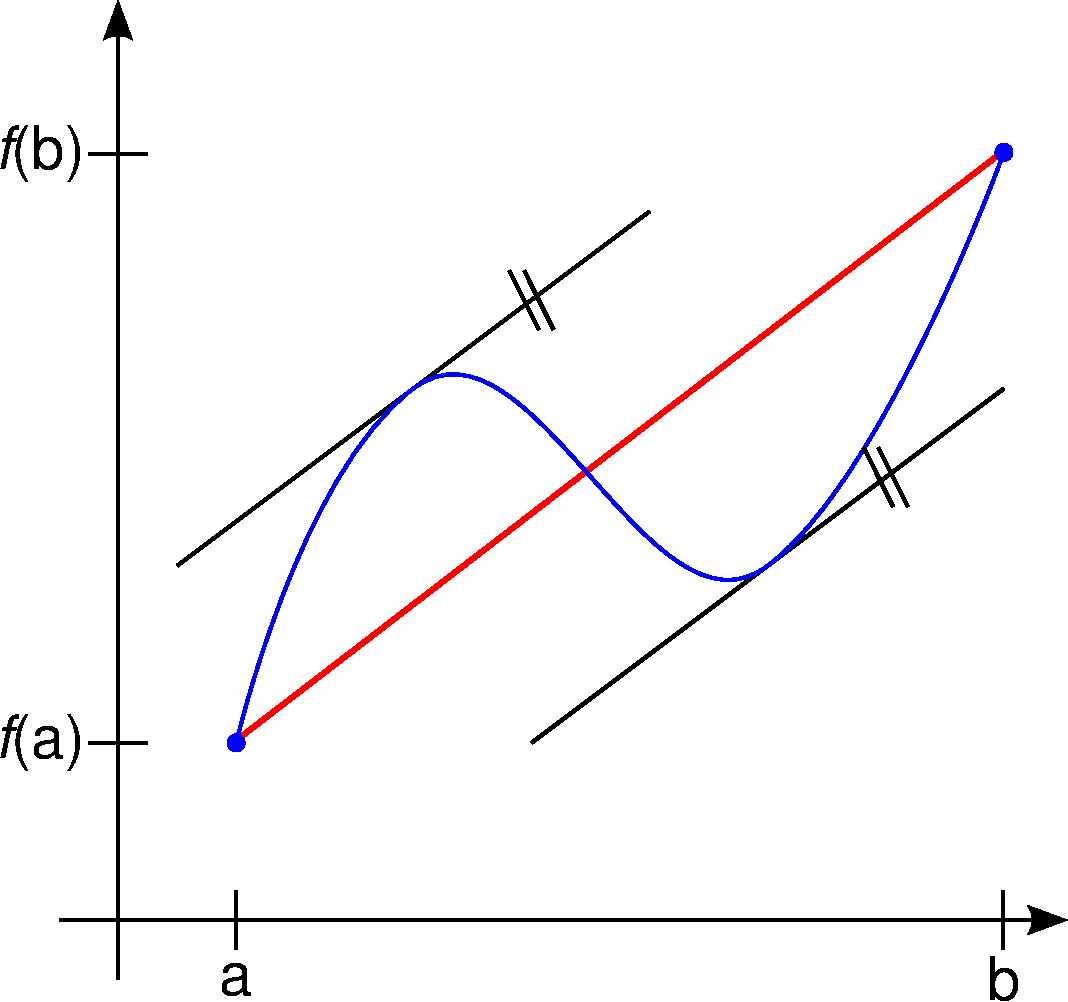
\includegraphics[width=0.4\textwidth]{include/20091201-3.pdf}
	\end{center}
\end{wrapfigure}
Vorraussetzung $f(a) = f(b)$ entfällt, aber es gilt: $f:[a,b] \rightarrow \mathbb{R}$ sei differenzierbar.
Es existiert ein $x_0$ mit $a < x_0 < b$ so dass die Sekantensteigung an den Endpunkten parallel zur Tangentensteigung in $x_0$ ist.
\begin{equation*}
	f'(x_0) = \frac{f(b) - f(a)}{b - a}
\end{equation*}
\begin{proof}
	Wende Satz von Rolle an auf:
	\begin{align*}
		h(x) &= f(x) - (x - a)\frac{f(b) - f(a)}{b - a} \\
		h'(x) &= f'(x) - 1\frac{f(b) - f(a)}{b - a} \\
		\intertext{Wie leicht zu sehen ist gilt:}
		h(a) &= f(a)\text{ und }h(b) = f(a) \\
		\intertext{aus dem Satz von Rolle folgt:}
		&\exists x_0 : h'(x_0) = 0 \Rightarrow f'(x_0) = \frac{f(b) - f(a)}{b - a}
	\end{align*}
\end{proof}
Folgerung für Differentialgleichungen:
\begin{equation*}
	\forall x : a < x < b \wedge f'(x) = 0 \Rightarrow f(x) = const \text{ einzige Lösung}
\end{equation*}
\begin{proof}[Beweis für 1. MWS]
	\begin{equation*}
		\exists x_0 : 0 = f'(x_0) = \frac{f(x) - f(a)}{x - a} \Rightarrow f(x) = f(a) = const
	\end{equation*}
	$\Rightarrow$ Konstante löst allgemein: $\dot s = 0 \Rightarrow s = c$.
\end{proof}

\subsubsection{Monotone Funktionen}
\begin{enumerate}
	\item $f'(x) \geq 0 \Rightarrow f$ ist monoton wachsend
	\item $f'(x) \leq 0 \Rightarrow f$ ist monoton fallend
\end{enumerate}
\begin{example}
	z. z. $f'(x_0) < 0 \Rightarrow x_1 > x_2 \Rightarrow f(x_1) < f(x_2)$
	$\frac{f(x_1) - f(x_2)}{\underbrace{x_1 - x_2}_{> 0}} = f'(x_0) < 0$
\end{example}

\subsubsection{Wendepunkte}
\begin{note}
	Die zweite Ableitung von $f$ beschreibt die Krümmung.
\end{note}
\begin{enumerate}
	\item $f''(x) > 0 \Rightarrow y = f(x)$ ist konvex (Linkskrümmung)
	\item $f''(x) < 0 \Rightarrow y = f(x)$ ist konkav (Rechtsskrümmung)
\end{enumerate}
Für den Wendepunkt gilt: $f''(x_0) = 0$ ist notwendig ($f'''(x_0) \neq 0$ ist hinreichend).
\begin{example}
	\begin{equation*}
		f(x) = x^3 \qquad f(0) = f'(0) = f''(0) = 0 \quad f'''(0) \equiv 6
	\end{equation*}
\end{example}

\lecture{2009-12-08}

\subsection{Regeln von L'Hospital}

unbestimmte Ausdrücke der Form $\frac 0 0$, $\frac \infty \infty$, $0 \cdot \infty$, $\ldots$ $\approx$ 1680 (Bernoulli)
\begin{example}\[ \liminfty[x]{\frac{\sin x} x} \]\end{example}

\noindent Hilfsmittel dazu: 2. Mittelwertsatz der Differentialrechnung
\begin{theorem}
  $f,g: \left[a,b\right] \to \mathbb R$ stetig und differenzierbar mit $g'(x) \neq 0$
  \[ g(a) \neq g(b) \implies \exists x_0: \frac{f(b)-f(a)}{g(b)-g(a)}=\frac{f'(x_0)}{g'(x_0)}  \]
\end{theorem}
\begin{note}
  nach 1. Mittelwertsatz
  \begin{equation*} \cfrac{\frac{f(b)-f(a)}{b-a}}{\frac{g(b)-g(a)}{b-a}} = \frac{f'(x_1)}{g'(x_2)} \end{equation*}
  mit $a < x_1, x_2 < b$, aber nicht $x_1 = x_2$
\end{note}
\begin{proof}
  Hilfsfunktion: $h(x) = f(x) - \frac{f(b)-f(a)}{g(b)-g(a)} \cdot (g(x)-g(a))$ stetig, differenzierbar
  \[
    \left.\begin{array}{r}h(a) = f(a)\\h(b)=f(a)\end{array}\right\} \leadsto \text{ Satz von Rolle: } \exists \textcolor{blue}{x_0}: h'(x_0) = 0
  \]
  \[ h'(x) = f'(x) - \frac{f(b)-f(a)}{g(b)-g(a)} \cdot g'(x) \]
  \[ \textcolor{blue}{x_0}: h'(x_0) = 0 = f'(x_0) - \frac{f(b)-f(a)}{g(b)-g(a)} \cdot g'(x_0) \]
  \[ \implies \frac{f(b)-f(a)}{g(b)-g(a)} = \frac{f'(x_0)}{g'(x_0)} \]
\end{proof}

\begin{theorem}[Regeln von L'Hospital]\label{theorem:hospital} Aus $f, g: \left]a,b\right[ \to \mathbb R$ differenzierbar mit $g'(x) \neq 0$, außerdem
  \begin{equation*} f(x), g(x) \xrightarrow[x \rightarrow a]{} 0 \text{ oder } f(x), g(x) \xrightarrow[x \rightarrow a]{} \infty \end{equation*}
  folgt:

  Falls der Grenzwert $\lim_{x \rightarrow a} \frac{f'(x)}{g'(x)}$ existiert, dann existiert auch der Grenzwert $\lim_{x \rightarrow a} \frac{f(x)}{g(x)}$, wobei
  \[ \lim_{x \rightarrow a} \frac{f(x)}{g(x)} = \lim_{x \rightarrow a} \frac{f'(x)}{g'(x)} \]
\end{theorem}
\begin{note}Nicht zu verwechseln mit der Quotientenregel! Zähler und Nenner werden getrennt voneinander differenziert.\end{note}
\begin{example}
  \begin{itemize}
    \item $\displaystyle\lim_{x \rightarrow 0} \underbrace{\left(\frac{\sin x} x\right)}_{\text{Form }\frac 0 0} =
      \lim_{x \rightarrow 0} \left(\frac{\cos x} 1\right) = 1$
    \item nützliche Umformungen
      \begin{footnotesize}\begin{align*}
        f(x) \cdot g(x) \text{ hat Form } 0 \cdot \infty &\implies f(x) \cdot g(x) = \frac{f(x)}{\frac 1 {g(x)}} \text{ hat Form } \frac 0 0 \\
        f(x) - g(x) \text{ hat Form } \infty - \infty &\implies f(x) \cdot g(x) \cdot \left( \frac 1 {f(x)} - \frac 1 {g(x)} \right) \text{ hat Form } \frac 0 0 \text { oder } \frac\infty\infty \\
      \end{align*}\end{footnotesize}
    \item
      \begin{align*}
        \lim_{x \rightarrow 0} \underbrace{\left( \frac 1 x - \frac 1 {\sin x} \right)}_{\text{Form } \infty - \infty}
        &= \lim_{x \rightarrow 0} \underbrace{\left( \frac{\sin x - x}{x \cdot \sin x} \right)}_{\text{Form } \frac 0 0} \\
        &= \lim_{x \rightarrow 0} \underbrace{\left( \frac{\cos x - 1}{x \cdot \cos x + \sin x} \right)}_{\text{Form } \frac 0 0} \\
        &= \lim_{x \rightarrow 0} \left( \frac{-\sin x}{2 \cdot \cos x - x\cdot \sin x} \right) \\
        &= \frac 0 2 = 0
      \end{align*}
  \end{itemize}
\end{example}

\subsubsection*{Nachtrag: Differentiation der $\euler$-Funktion $\euler^x$}

Einführung $\euler^x$ als Folgengrenzwert:
\begin{equation*}
  \euler^x = \liminfty{\left( 1+\frac x n\right)^n}
\end{equation*}
Definition $g(x) = \liminfty{\left( 1+\frac x n\right)^n}$, stetig differenzierbar
\begin{align*}
  \implies g'(x) &= \frac n n \cdot \left( 1+\frac x n\right)^{n-1} = \left( 1+\frac x n\right)^{n-1} \\
  &= \left( 1+\frac x n\right)^{-1}\cdot \left( 1+\frac x n\right)^{n} \\
  &= \left( 1+\frac x n\right)^{-1}\cdot g(x) \\
  &\xrightarrow[n \rightarrow \infty]{x: \text{ fest}} g(x)
\end{align*}

\begin{note}
  $\euler$-Funktion ist so gebaut, dass Ableitung $=$ Funktion $\leadsto$ gewöhnliche Differentialgleichung:
  \begin{align*}
    \dot y = y &\implies y(t) = c\cdot \euler^t \\
    \lambda \in \mathbb R\quad \dot y = \lambda y &\implies y(t) = c \cdot \euler^{\lambda t}
  \end{align*}
  (wegen $\frac\diff{\diff t} \euler^{h(t)} = h'(t)\cdot\euler^{h(t)}, h(t) = \lambda t$)

\end{note}

\subsection{Kurvendiskussion $y = f(x)$}

\begin{enumerate}
  \item Definitionsbereich, Wertebereich
  \item Symmetrien (gerade, ungerade)
  \item Stetigkeit, Polstellen
  \item Nullstellen% (siehe \todo{Referenz auf 7.8 bzw. 2.3.8})
  % LH: Referenz wäre sinnlos, in 7.8 geht es um Umkehrfunktionen
  \item $f'$ berechnen, $f' = 0$ Nullstellen
  \item Extremwerte: innere Extrema, Randextrema, Monotoniebereiche
  \item $f''$ berechnen, $f'' = 0$ Nullstellen
  \item Wendepunkte, konvexe/konkave Bereiche
  \item asymptotisches Verhalten $x \rightarrow \pm\infty$
  \item Graph
\end{enumerate}

\subsection{Gewöhnliche Differentialgleichungen -- 2. Teil}

\begin{wrapfigure}{r}[1cm]{.4\textwidth}
  \centering
  \begin{tikzpicture}[scale=0.5,y=0.6cm]
    \fill[color=blue!10] (-4,-2) -- (-4,19) -- (4,19) -- (4,-2);

    % x-Achse
    \draw[->] (-5,0) -- (5,0) node[below] {$x$};
    \draw (-4,0.2) -- (-4,-0.2) node[below right] {$-a$};
    \draw (4,0.2) -- (4,-0.2) node[below left] {$a$};

    % y-Achse
    \draw[->] (0,-1) -- (0,19) node[left] {$y$};

    % Landmarkierung
    \foreach \x in {-1,...,18}
      \draw[color=gray] (-5,\x-1) -- (-4.0,\x);

    \foreach \x in {-1,3,4,...,15,18}
      \draw[color=gray] (5,\x-1) -- (4,\x);

    % Flussgrenzen
    \draw (-4,-1) -- (-4,18);
    \draw (4,-1) -- (4,18);

    % Flussgeschwindigkeitsfunktion
    \draw[domain=-4:4] plot [id=flussgeschw, samples=50] function {6*(1-(x**2)/(4**2))} node[above right] {Geschwindigkeit};
    % Geschwindigkeitsvektoren
    \foreach \x/\y in {-4/0, -3/2.625, -2/4.5, -1/5.625, 0/6, 1/5.625, 2/4.5, 3/2.625, 4/0}
      \draw[->] (\x,0) -- (\x,\y);

    % Abdriftsfunktion
    \draw[domain=-4:4] plot [id=abdrift, samples=50] function {3*(x-(x**3)/(3*4**2))+8} node[right] {Abdrift} node[above left] {b};
  \end{tikzpicture}
\end{wrapfigure}
% Derbster Hack aller Zeiten:
$ $ % Ich weiß nicht, was hier passiert. Anders geht es aber nicht.
% siehe http://www.cis.hut.fi/ntvuok/scripts.php --LH
\begin{example}[Hund springt in Eisbach und driftet ab]\flush
  \begingroup
  \newcommand{\kmh}{\ensuremath{\,\textstyle \frac{\text{km}}{\text{h}}}}
  \begin{itemize}
    \item $v_0$ maximale Geschwindigkeit des Wasser
      \begin{equation*} v_0 = 6 \kmh \end{equation*}
      Wahl: Parabelprofil
      \begin{equation*} v_\text{F}(x) = v_0 \cdot \left( 1 - \frac{x^2}{a^2} \right) \end{equation*}
      \begin{equation*} v(a) = v(-a) = 0 \end{equation*}
    \item Hund: konstante Eigengeschwindigkeit
      \begin{align*}
        v_H &= 2 \kmh \\
        v_H &\parallel \text{$x$-Achse}
      \end{align*}
  \end{itemize}
  \par
  \begin{itemize} % hack
    \item Fragen: Welche Bahn schwimmt der Hund? Wie groß ist seine Abdrift $b$?
      \begin{equation*} \left. \tan \alpha = \frac{v_\text{F}}{v_\text{H}} = y'(x) \quad\right\rangle\quad y'(x) = \frac{v_0}{v_\text{H}} \cdot \left( 1 - \frac{x^2}{a^2}\right)\end{equation*}
    \item Erraten der Lösung
      \begin{equation*}
      y(x) = c + \frac{v_0}{v_\text{H}} \cdot \left( x - \frac{x^3}{3a^2}\right)
      \end{equation*}
    \item Abdrift
      \begin{align*}
        b = \underbrace{y(a)}_{\parbox{16mm}{\centering\scriptsize landet der Hund}} -\underbrace{y(-a)}_{\parbox{16mm}{\centering\scriptsize startet der Hund}} &= \ds\frac{v_0}{v_\text{H}} \cdot \underbrace{\left( \left( a - \frac{a^3}{3a^2}\right) - \left( -a + \frac{a^3}{3a^2}\right) \right)}_{2a - \frac 2 3 a} \\
        &= \ds\frac 4 3 \cdot \frac{v_0}{v_\text{H}}\cdot  a
      \end{align*}
      in Zahlen:
      \begin{equation*}
        b = \frac 4 3 \cdot \frac {6 \kmh}{2 \kmh} \cdot 4 \,\text{m} = 16 \,\text{m}
      \end{equation*}
  \end{itemize}
  \endgroup
\end{example}


\lecture{2009-12-09}

% EISBACH %
\noindent $y'(x) = f(x)$ einfache Differentialgleichung, da $f$ nur Funktion von $x$ und nicht von $y$ ist. 
Daher ist das Erraten der Lösung als Integral möglich.

\begin{equation*}\leadsto y(x) = \int_{-a}^{+a} \! f(x) \, \diff x\end{equation*}
Allgemeines Anfangswertproblem:
\begin{equation*}\dot y(t) = f(t, y) \qquad y \in \mathbb{R}^n \qquad y(t_0) = y_0\end{equation*}
Eisbach: allgemeines AWP linear 1. Ordnung/Typs
\[ y'(x) = p(x)\cdot y + q(x)\qquad y \in \mathbb{R}^1 \]

\subsection{Umkehrfunktionen}
$f: I \to \mathbb{R}$ stetig (evtl. auch etwas weniger stückweise stetig oder auch etwas mehr differenzierbar)

\begin{definition}[Umkehrbarkeit]
    $f$ heißt umkehrbar über $D \subseteq I$, falls für alle $y \in f(D)$ gilt:
    Die Gleichung $y=f(x)$ hat genau eine Lösung $x$
    \begin{equation*}
        \left.
        \begin{array}{r}
            g:\underbrace{f(D)}_{\subseteq \mathbb{R}} \to D x= g(y) \Leftrightarrow y=f(x) \\
            g: \text{Umkehrfunktion zu }f: g=f^{-1}
        \end{array}
        \right\}
        \begin{array}{l}
            g \circ f = f \circ g = id\\
            g(f(x)) = x\\
            f(g(y)) = y
        \end{array}
    \end{equation*}
\end{definition}

\begin{example}
\begin{enumerate}
    \item $f(x)=ax + b \implies g(y) = \frac{1}{a} \cdot (y-b) $
    \begin{center}
        \begin{tikzpicture}[]
         \draw[->,semithick] (-2.5,0) -- (2.5,0) node[below]{x};
         \draw[->,semithick] (0,-0.5) -- (0,3) node[left]{y};
         \draw[domain=-2:2] plot [id=umkehr_a, samples=50] function {0.6*x+1};
         \node at (1.5,0.5) {$y=a\cdot x + b$};
        \end{tikzpicture}
    \end{center}
    \item
        $
            \left.
            y=f(x)=x^2 \implies
            \right\{
            \begin{array}{l}
            x \geq 0: g(y) = +\sqrt{y}\\
            x < 0: g(y) = -\sqrt{y}
            \end{array}
        $
    \begin{center}
        \begin{tikzpicture}[]
         \draw[->,semithick] (-2.5,0) -- (2.5,0) node[below]{x};
         \draw[->,semithick] (0,-0.5) -- (0,4.25) node[left]{y};
         \draw [dashed] (-1,0) -- (-1,1) -- (1,1) -- (1,0);
         \draw (-1,0) -- (-1,-0.2) node[below] {$\hat{x}$};
         \draw (1,0) -- (1,-0.2) node[below] {$x$};
         \draw[domain=-2:2] plot [id=umkehr_b, samples=50] function {x**2};
         \node at (0.7,2) {$y=x^2$};
        \end{tikzpicture}
    \end{center}
\end{enumerate}
\end{example}
offensichtlich \todo{Graph}: (streng) monotone Funktionen erlauben Umkehrung 

monotone Funktionen werden an $y=x$ gespiegelt. $\leadsto g=f^{-1}$

\subsubsection*{Hauptsatz zu Umkehrfunktionen}
\begin{enumerate}
    \item Jede streng monotone Funktion $f(x)$ ist umkehrbar.
    \item $f$ und $g=f^{-1}$ gegeben $\implies$ Graph von $g$ ist symmetrisch zu Graph von $f$ bzgl. $y=x$. (siehe Skizzen)
    \item
        $
            \left.
            \begin{array}{l}
            f:I \to \mathbb{R} \text{ differenzierbar und umkehrbar}\\
            g:f(I) \to \mathbb{R} \text{ Umkehrfunktion}\\
            \text{es gilt: g differenzierbar und } g'(x) = \frac{1}{f'(g(x))}
            \end{array}
            \right\}
            \begin{array}{l}
            \text{Kettenregel } f(g(x)) = x\\
            \text{differenziere } f'(g(x)) \cdot g'(x) = 1
            \end{array}
        $
\end{enumerate}

\begin{example}[Umkehrfunktionen]
\begin{enumerate}

    \item n-te Wurzel für rationale Exponenten:\\
        bisher $y = \sqrt[n]{x} \quad n \in \mathbb{N} \Leftrightarrow y^n = x \quad
            \begin{cases}
                x \geq 0 & \text{$n$ gerade} \\
                x < 0 & \text{$n$ ungerade}
            \end{cases}
        $\\
        Umschreibung:
        \[\sqrt[n]{x} = x^{\frac{1}{n}}\]
        Potenzbildung:
        \[x^{\frac{m}{n}} := \left(x^{\frac{1}{n}}\right)^m\]
        Ableitung:
        \begin{align*}
            f(x)=x^n \qquad g(x) = x^{\frac{1}{n}}\\
            g'(x)=\frac{1}{n \cdot \left(x^{\frac{1}{n}}\right)^{n-1}}=\frac{1}{n} \cdot x^{\left(\frac{1}{n}-1\right)}
        \end{align*}
        Kettenregel: Exponent $\frac{m}{n}$ zu berechnen:\\
        \[ \frac{\diff}{\diff x}x^{\frac{m}{n}} = \frac{m}{n} \cdot x^{\left(\frac{m}{n}-1\right)}\]
    \item Arkus-Funktion:\\
        trigonometrische Funktionen sind nicht \emph{global} umkehrbar\\
        Umkehrung möglich in $-\frac{\pi}{2} \leq x \leq \frac{\pi}{2}$
        \begin{definition}[Umkehrfunktion von $\sin x$]
        Die Umkehrfunktion von $\sin x$ in $[-\frac{\pi}{2}, \frac{\pi}{2}]$ ist $\arcsin x\,:[-1,1]\to[-\frac{\pi}{2}, \frac{\pi}{2}]$
        \end{definition}
        Ableitung:
        \[\frac{\diff}{\diff x}\arcsin x=\frac{1}{\underbrace{\cos}_{f'}(\underbrace{\arcsin x}_{g})}\]
        Mit Pythagoras $1=\sin^2 x+\cos^2 x \implies \cos x=\sqrt{1-\sin^2 x}$ (wegen Abschnitt "`$+\sqrt{\,}$"') folgt:
        \[\frac{\diff}{\diff x}\arcsin x = \frac{1}{\sqrt{1-\sin^2(\arcsin x)}} = \frac{1}{\sqrt{1-x^2}}\]
        Analog für $\cos x, \tan x, \cot x$:
        % note: Sinus und Cosinus dürften bekannt sein -> habe die Graphen weggelassen
        \begin{align*}
            \arccos x&: [-1,1]\to[0,\pi]\\
            \frac{\diff}{\diff x} \arccos x &= \frac{-1}{\sqrt{1-x^2}}\\
            \frac{\diff}{\diff x} \arctan x &= \frac{1}{1+x^2}
        \end{align*}

\end{enumerate}
\end{example}

\subsection{Exponentialfunktion, Logarithmusfunktion}
\subsubsection*{Eigenschaften von $\euler^x$}
\begin{itemize}
    \item Definiert aus Grenzwert $\ds\lim_{n \to \infty}\left(1+\frac{x}{n}\right)^n =: \euler^x = \exp(x)$
    \item Ableitung $\frac{\diff}{\diff x}\euler^x = \euler^x$ (hebt $\euler^x$ aus allen $f(x)$ heraus)
    \item Positivität: $\euler^0 = 1 \qquad \euler^x > 0 \, \forall x \in \mathbb{R}$
            \[\euler^1=\euler=2,718281828459... \text{Euler'sche Zahl}\]
    \item Wachstum: $\ds\lim_{n \to \infty} \euler^x = \infty$
            \[\lim_{n \to -\infty} \euler^x = \lim_{n \to \infty} \frac{1}{\euler^x} = 0\]
    \item Vergleich mit Wachstum von $x^n$:
        \begin{align*}
            \lim_{n \to \infty} \frac{\euler^x}{x^n} = \left(\frac{\infty}{\infty}\right) = \lim_{n \to \infty}\frac{\euler^x}{n\cdot x^{n-1}} = \left(\frac{\infty}{\infty}\right) = \ldots =  \lim_{n \to \infty}\frac{\euler^x}{n!} = \infty
        \end{align*}
        "`$\euler$-Funktion wächst schneller als jede Potenz von $x^n$"' (L'Hospital, Seite \pageref{theorem:hospital})
    \item Umkehrbarkeit: $\euler^x$ ist monoton $\implies \euler^x$ ist umkehrbar
\end{itemize}

\begin{center}
    \begin{tikzpicture}[]
     \draw[->,semithick] (-2.5,0) -- (3,0) node[below]{x};
     \draw[->,semithick] (0,-0.5) -- (0,4) node[left]{y};
     
     \draw[domain=-2.5:1.3] plot [id=euler, samples=400] function { exp(x)};
     \node at (2,1.5) {$y = \euler^x$};
     \draw (-2pt,1) -- (2pt,1) node[left] {1};
     \draw (1,2pt) -- (1,-2pt) node[below] {1};
     \draw (-1,2pt) -- (-1,-2pt) node[below] {-1};
    \end{tikzpicture}
\end{center}

\begin{definition}[Logarithmus Naturalis]
    Die Umkehrfunktion von $\euler^x$ ist der natürliche Logarithmus $\ln x$.
    \begin{align*}
        \ln 1 = 0 \qquad \ln \euler = 1\\
        0 < x < 1 &\implies \ln x < 0\\
        x > 1 &\implies \ln x > 0\\
        \frac{d}{dx}\ln x = \frac{1}{\underbrace{\exp}_{f'}\underbrace{(\ln x)}_{g}} = \frac{1}{x}
    \end{align*}
\end{definition}

\begin{center}
    \begin{tikzpicture}[]
     \draw[->,semithick] (-0.5,0) -- (5.5,0) node[below]{x};
     \draw[->,semithick] (0,-2.5) -- (0,2.5) node[left]{y};
     
     \draw[domain=0.1:5] plot [id=log_ln, samples=400] function { log(x)};
     \node at (2,1.5) {$y = \ln x$};
     \draw [dash pattern=on 1pt off 1pt] (0,1)-- (2.718,1);
     \draw [dash pattern=on 1pt off 1pt] (2.718,0)-- (2.718,1);
     \draw (-2pt,1) -- (2pt,1) node[left] {1};
     \draw (1,2pt) -- (1,-2pt) node[below] {1};
     \draw (2.718,2pt) -- (2.718,-2pt) node[below] {$\euler$};
    \end{tikzpicture}
\end{center}

\subsubsection*{Rechenregeln}
\begin{enumerate}
    \item $\ln(x\cdot y) = \ln x + \ln y$
    \item $\ln\left(\frac{x}{y}\right) = \ln x - \ln y \quad (y \neq 0)$
\end{enumerate}

\subsubsection*{Allgemeine Potenzen zu $x^\alpha$ für $\alpha \in \mathbb{R}$}
Idee: allgemeine Potenzfunktion $a^x$ mit $ a > 0,\, x \in \mathbb{R}$:
\begin{equation*} a^x = \exp(\ln a^x) = \exp (x \ln a) = \euler^{x \ln a}\end{equation*}
Berechne $x^\alpha$ und die Ableitung ($x > 0$):
\[ \frac{\diff}{\diff x} x^\alpha = \frac{\diff}{\diff x} \euler^{\alpha \ln x} = \alpha \underbrace{\euler^{\alpha \ln x}}_{x^\alpha} \cdot \frac{1}{x} = \alpha \cdot x^\alpha \cdot \frac{1}{x} = \alpha \cdot x^{\alpha-1}\]
\subsubsection*{Rechenregeln}
\begin{enumerate}
    \item $a^x \cdot a^y = a^{(x+y)}$
    \item $(a^x)^y = a^{\left(x\cdot y\right)}$
    \item $(a\cdot b)^x = a^x \cdot b^x$
    \item $\ln(a^x) = x \cdot \ln a \quad | a > 0$
\end{enumerate}

\begin{definition}[Hyperbelfunktion]
    \begin{align*}
        \sinh x = \frac{\euler^x - \euler^{-x}}{2}\\
        \cosh x = \frac{\euler^x + \euler^{-x}}{2}
    \end{align*}
\end{definition}
\begin{center}
    \begin{tikzpicture}[]
     \draw[->,semithick] (-2.5,0) -- (2.5,0) node[below]{x};
     \draw[->,semithick] (0,-2) -- (0,3.5) node[left]{y};
     \draw[blue,domain=-1.3:1.8] plot [id=sinh, samples=50] function { sinh(x)};
     \draw[red,domain=-1.8:1.8] plot [id=cosh, samples=50] function { cosh(x)};
     \node[color=blue] at (1.5,0.6) {$\sinh x$};
     \node[color=red] at (-0.7,2.2) {$\cosh x$};
    \end{tikzpicture}
\end{center}

\lecture{2009-12-15}

Es gilt:
\begin{equation*}
	\cosh^2 x - \sinh^2 x = 1
\end{equation*}

\subsubsection*{Umkehrfunktionen}

\begin{equation*}
	\left.
	\begin{aligned}
		&\sinh x \text{ ist streng monoton } \leadsto \text{ umkehrbar} \\
		&\sinh x : \mathbb{R} \rightarrow \mathbb{R}
	\end{aligned}
	\right\} \arsinh x \text{ (Areasinus hyperbolicus)}
\end{equation*}

\paragraph{Explizite Angabe von $\arsinh x$}
\begin{align*}
	y &= \sinh x = \frac{\euler^x - \euler^{-x}}{2} \text{ Auflösen nach $x$}\\
	\implies 2y &= \euler^x - \euler^{-x} \quad| \cdot \euler^x \\
	\implies 2y \euler^x &= \euler^x \euler^x - \underbrace{\euler^x \euler^{-x}}_{=1} \\
	\implies \euler^{2x} - 2y\euler^x &= 1 \\
	\implies (\euler^x - y)^2 &= 1 + y^2 \\
	\implies \euler^x &= y + \sqrt{1 + y^2} \\
	\implies x &= \ln (y + \sqrt{1 + y^2}) = \arsinh y
\end{align*}

\paragraph{Folgerung}
\begin{multline*}
	\frac{\diff}{\diff x} \arsinh x = \frac{1}{x + \sqrt{1 + x^2}}\left(1 + \frac{1 \cdot 2x}{2\sqrt{1 + x^2}}\right) = \frac{1}{x + \sqrt{1 + x^2}} \left(1 + \frac{x}{\sqrt{1 + x^2}} \right) = \\
	= \frac{1}{x + \sqrt{1 + x^2}} \left(\frac{\sqrt{1 + x^2} + x}{\sqrt{1 + x^2}}\right) = \frac{1}{\sqrt{1 + x^2}}
\end{multline*}

\subsection{Fixpunkte, Iterationsverfahren}
Einer der ersten Schritte der Kurvendiskussion ist die Nullstellenbestimmung.

\subsubsection*{Nullstelle als Fixpunkt formulieren}

\begin{definition}
	$x^* \in [a, b]$ heißt Fixpunkt, falls gilt: $f: [a, b] \rightarrow \mathbb{R}: f(x^*) = x^*$
\end{definition}
\begin{lemma}
	Jeder Fixpunkt $x^*$ von $f$ ist Nullstelle der Funktion $g(x) = f(x) - x$. \\
	Umgekehrt: Jede Nullstelle von $f$ ist Fixpunkt von $g(x) = f(x) + x$.
\end{lemma}
\begin{definition}[Einstellige Fixpunktiteration]\flush
	\begin{equation*}
		x_{n + 1} = f(x_n) \qquad n \geq 0 \quad \text{zu gegebenem $x_0$}
	\end{equation*}
	(Im Folgenden sind alle Fixpunktiterationen einstellig.)
\end{definition}

\subsubsection*{Iterationsverläufe}
\begin{enumerate}
	\item $f(x) : 0 < f'(x) < 1$ (konvergente Iteration)
	\begin{center}
		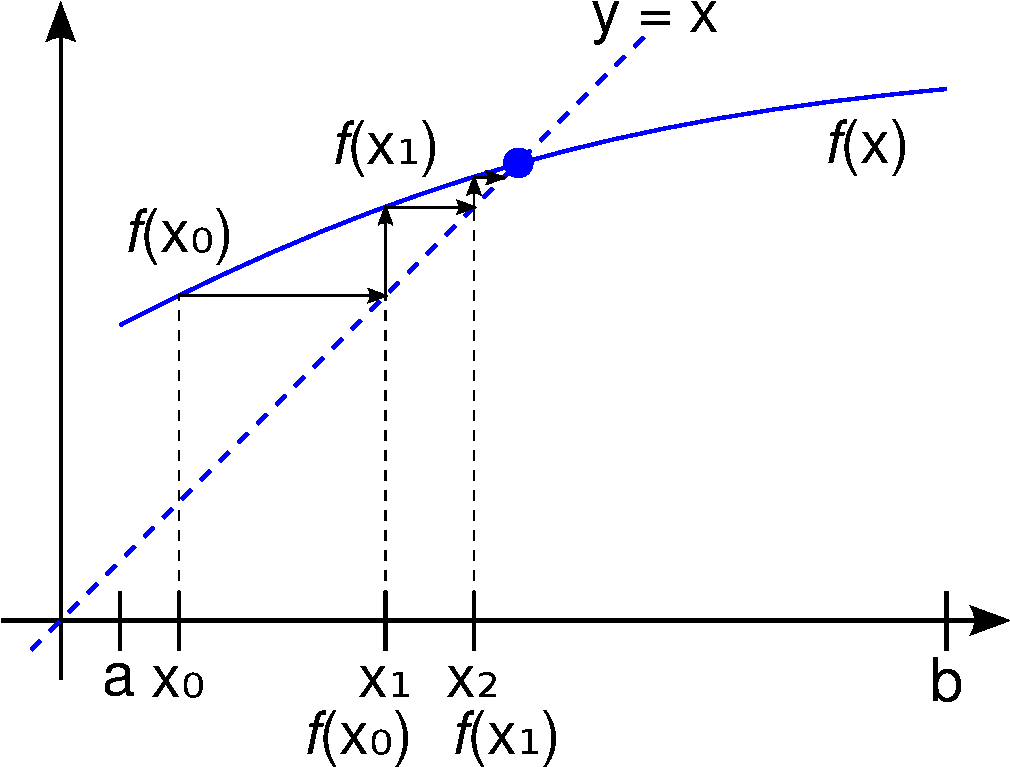
\includegraphics[width=0.4\textwidth]{include/20091215-1.pdf}
	\end{center}
	\item $f(x) : -1 < f'(x) < 0$ (konvergente Iteration)
	\begin{center}
		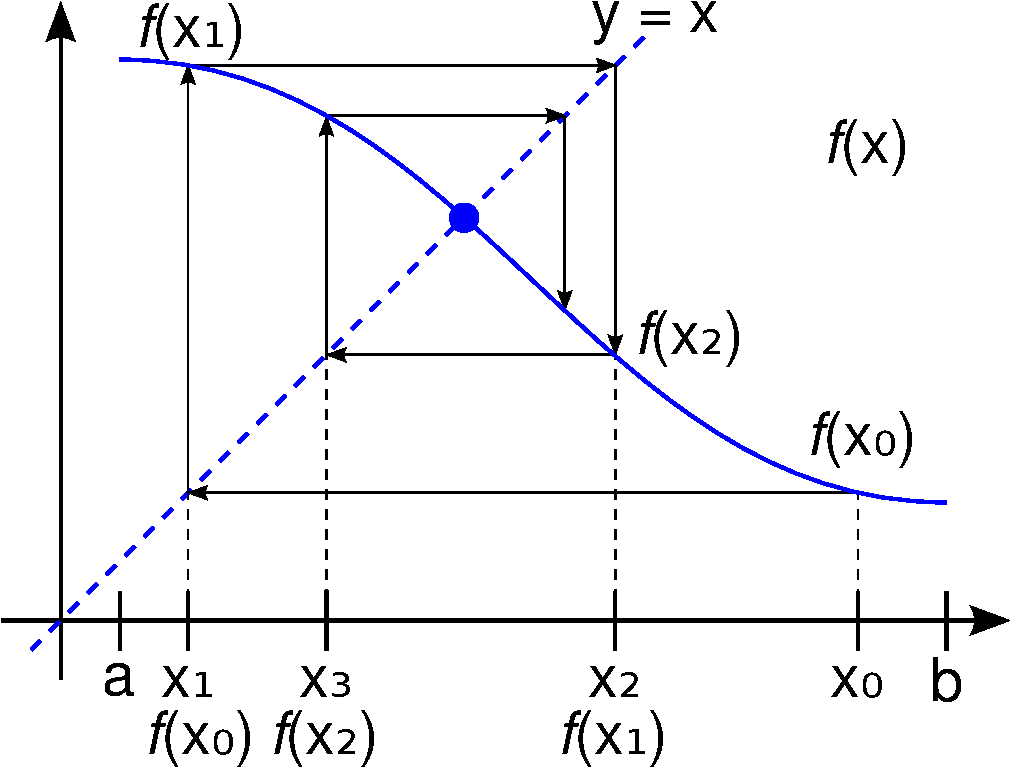
\includegraphics[width=0.4\textwidth]{include/20091215-2.pdf}
	\end{center}
	\item $f(x) : f'(x) > 1$ (divergente Iteration)
	\begin{center}
		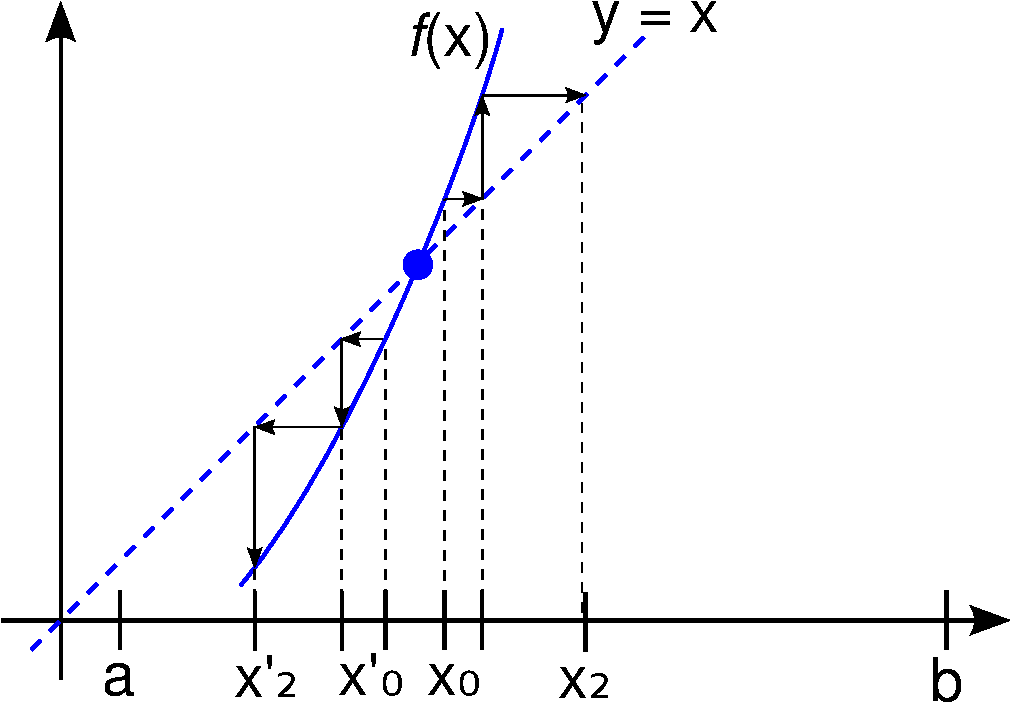
\includegraphics[width=0.4\textwidth]{include/20091215-3.pdf}
	\end{center}
\end{enumerate}

\begin{definition}[Lipschitz-Stetigkeit]
	Eine stetig differenzierbare Funktion $f: [a, b] \rightarrow \mathbb{R}$ heißt Lipschitz-stetig auf $[a, b]$, falls eine Lipschitz-Konstante $L$ existiert, mit
	\begin{equation*}
		|f(x_1) - f(x_2)| \leq L |x_1 - x_2| \qquad x_1, x_2 \in [a, b]
	\end{equation*}
	$f$ heißt \emph{kontrahierend}, falls $L < 1$.
\end{definition}
\begin{note}
	Aus dem 1. MWS folgt: $L = \underset{x \in ]a, b[}{\max} |f'(x)|$
\end{note}

\subsubsection*{Fixpunktsatz von Banach}
Wesentliche Voraussetzung: $f$ ist kontrahierend $\implies x_{n + 1} = f(x_n)$ ist konvergent
\begin{wrapfigure}[10]{r}{0.4\textwidth}
 	\centering
	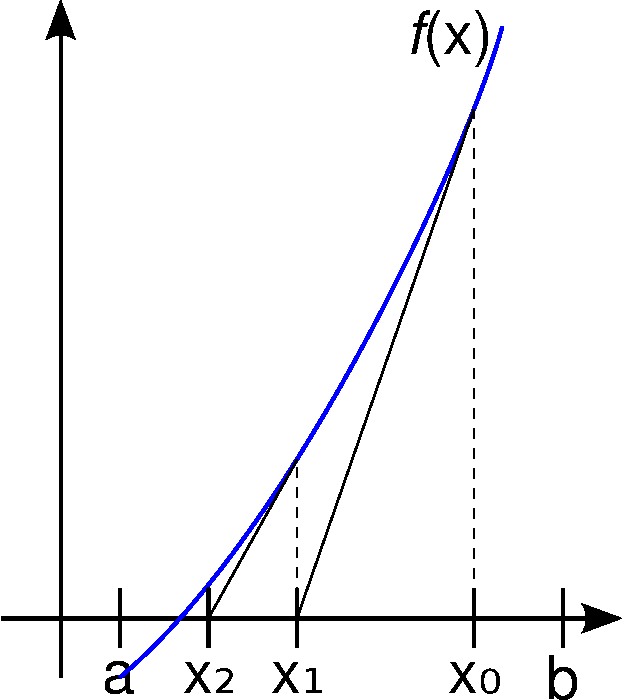
\includegraphics[width=0.4\textwidth]{include/20091215-4.pdf}
\end{wrapfigure}

\begin{note}
	Für nicht-kontrahierende Funktionen ist das Newton-Verfahren eine Abhilfe zur Nullstellensuche:
	\begin{align*}
		\text{Startwert}\:&:\: x_0 \\
		n \geq 0\:&:\:x_{n + 1} = x_n - \frac{f(x_n)}{f'(x_n)}
		\intertext{(Schnittgleichung: Tangente $\leftrightarrow$ x-Achse)}
	\end{align*}

	Das Newton-Verfahren ist (im Wesentlichen als einziges Verfahren) auf $\mathbb{R}^n$ verallgemeinerbar:
	\begin{align*}
		x_{n + 1} &= x_n + \Delta x_n \\
		\Diff f(x_n) \Delta x_n &= -f(x_n) \\
		\Delta x_n &= -\Diff f^{-1}(x_n) f(x_n)
	\end{align*}
\end{note}


\lecture{2009-12-16}

\chapter{Reihen, Potenzreihen, Taylorreihen}

\section{Schneeflockenkurve nach Koch, Reihen}

Passend zu Weihnachten: Konstruktion einer Schneeflocke mit $\infty$-großem Umfang aber endlicher Fläche.

\subsubsection*{Konstruktion}
Start: gleichseitiges $\triangle s_1$ der Kantenlänge 1: Fläche $F_1$, Umfang $U_1$

\begin{center}
    \begin{tikzpicture}[scale=1, x=1cm, y=1cm]
	    \draw (-2, 0) -- (2, 0) -- (0, 3.4) -- (-2, 0);
	    \draw (0, 0) -- (0, 3.4);
	    \draw (0, 1.6) node [right] {$h_1$};
	    \draw (1, 1.6) node [right] {$1$};
	    \draw (0, 0) node [below] {$1$};
	    \draw (-1, 1.6) node [left] {$1$};
    \end{tikzpicture}
\end{center}

\begin{align*}
    g_1 &= 1 \\
    h_1^2 + \left(\frac{1}{2})\right)^2 &= 1^2 \\
    F_{\triangle} &= \frac{g h}{2} \\
    \Rightarrow h_1 &= \frac{1}{2} \sqrt{3}
\end{align*}

zu $\triangle s_1$:
\begin{align*}
    U_1 &= 3 g_1 = 3 \\
    F_1 &= \frac{1}{4} \sqrt{3} \hspace{20px} \text{($g_1 h_1$: 2)}
\end{align*}

\subsubsection*{1. Schritt (Rekursion für alle Schritte):}

Drittle jede Seite und errichte über dem Mittelstück ein gleichseitiges $\triangle$

\begin{center}
    \begin{tikzpicture}[decoration=Koch snowflake, scale=1, x=1cm, y=1cm] % wtf tikz
		\draw decorate{(-2, 0) -- (0, 3.4) -- (2, 0) -- (-2, 0)};
	\end{tikzpicture}
\end{center}

\begin{align*}
    F_2 &= F_1 + 3 F_{\text{kl} \triangle} \\
    F_{\text{kl} \triangle} &= \frac{1}{2} g_2 h_2 \\
    &= \frac{1}{2} \frac{1}{3} h_2 \\
\\
    h_2^2 + \left( \frac{1}{6} \right)^2 &= \left( \frac{1}{3} \right)^2 \\
    \Rightarrow h_2 &= \frac{1}{3} \sqrt{ \frac{3}{4} } \\
\\
    \Rightarrow F_{\text{kl} \triangle} &= \frac{1}{9} \left( \frac{1}{4} \sqrt{3} \right)
\\
    U_2 &= U_1 + 3 g_2 = 4
\end{align*}

\subsubsection*{2. (allgemeiner) Schritt:}
Drittelung über alle Begrenzungsgeraden von $s_2$ liefert den 18-zackigen Stern $s_3$

\begin{center}
    \begin{tikzpicture}[decoration=Koch snowflake, scale=1, x=1cm, y=1cm]
		\draw decorate{ decorate{(-2, 0) -- (2, 0)} };
	\end{tikzpicture}
\end{center}


Konstruktionsprinzip: 3 Zacken werden vervierfacht

\begin{align*}
    F_3 &= F_2 + 3*4*F_{\text{neu}} \\
    U_3 &= U_2 + 12 * \frac{1}{9} \\
\\
    F_{\text{neu}} &= \frac{1}{2} h_3 g_3 \\
    &= \frac{1}{4} \sqrt{3} \frac{1}{9^2}
\end{align*}

allgemein:
$n > 2$:
\begin{align*}
    F_n = F_{n-1} + 3 * 4^{n-2} \left( \frac{1}{4} \sqrt{3} \frac{1}{9^{n-1}} \right) \\
    U_n = U_{n-1} + \left( \frac{4}{3} \right)^{n-2}
\end{align*}

Beweis: vollständige Induktion, Beweismittel sind bereits erläutert

Auflösen der 2-Term-Rekursion:

\begin{align*}
    F_n &= \frac{1}{4} \sqrt{3} \left\{ 1 + \frac{1}{3} + \frac{1}{9} \sum_{k=1}^{n-2} \left( \frac{4}{9} \right)^k \right\} \\
    U_n &= 4 + \sum_{k=1}^{n-2} \left( \frac{4}{3} \right)^k
\end{align*}

\section{Begriffe zu Reihen}

Idee: Führe die Form $\sum_{k=0}^{\infty} a_k$ auf Folgen zurück!

\begin{definition} Zu jeder reellen Zahlenfolge $(a_n)_{n \in \mathbb{N}}$ heißt die Folge
\begin{equation*}
    s_n = \sum_{k=1}^n a_k = a_1 + \dots + a_n
\end{equation*}
die n-te Partialsumme der Reihe $\sum_{k=1}^{\infty} a_k$
\end{definition}

Grenzwert der Reihe $\equals$ Folgengrenzwert der Partialsummen \\
% noch zu leisten: Interpretation/Anwendung

\begin{definition}
Eine Reihe $\sum_{k=1}^{\infty} a_k$ heißt konvergent (divergent) falls die Folge der Partialsummen konvergent (divergent) ist.
\end{definition}

Für Konvergenz/Divergenz-Untersuchungen haben wir \emph{nur} ein \emph{zentrales Werkzeug}: die geometrische Reihe
\begin{equation*}
    \left. \sum_{k=1}^{\infty} x^k = \right\{ \begin{array}{cll}
                                                    \frac{1}{1-x} & |x| \le 1 &\text{Konvergenz}\\
                                                    \infty & |x| \geq 1 & \text{Divergenz}
                                                \end{array}
\end{equation*}

\subsubsection*{Anwendung: Schneeflockenkurve}
\begin{align*}
    F_n: x &= \frac{4}{9} \le 1 \Rightarrow \text{Konvergenz, endliche Fläche} \\
    U_n: x &= \frac{4}{3} \ge 1 \Rightarrow \text{Divergenz, unendliche Fläche}
\end{align*}

\subsubsection*{Intuitive Kriterien}

\begin{enumerate}
    \item Notwendig für Konvergenz der Reihe: Reihenelemente $(a_n)_{n \in \mathbb{N}}$ bilden eine \emph{Nullfolge}
    \item umgekehrter Schluss: $(a_n)_{n \in \mathbb{N}}$ $\not\Rightarrow$ Konvergenz der Reihe\\
        Gegenbeispiel: $\sum_{k=1}^{\infty} \frac{1}{k} \rightarrow \infty $ (siehe frühere 2er-Potenzen) \\
        harmonische Reihe divergent!
\end{enumerate}

\begin{note}
    $(a_n)_{n \in \mathbb{N}}$ Nullfolge ist \emph{notwendig} aber nicht \emph{hinreichend}.
\end{note}

\subsubsection*{Rechenregeln für konvergente Reihenelemente}
\begin{enumerate}
    \item \begin{equation*} a = \sum_{k=1}^{\infty} a_k, b = \sum_{k=1}^{\infty} b_k \end{equation*}
        \begin{equation*}\Rightarrow \sum_{k = 1}{\infty} \left( a_k \pm b_k \right) = \sum_{k=1}^{\infty} a_k \pm \sum_{k=1}^{\infty} b_k = a \pm b
        \end{equation*}
    \item \begin{equation*}c \in \mathbb{R} \hspace{10px} \sum_{k=1}^{\infty} c a_k = c \sum_{k=1}^{\infty} a_k = c a \end{equation*}
    \item \begin{equation*}a_k \leq b_k \Rightarrow \sum_{k=1}^{\infty} a_k \leq \sum_{k=1}^{\infty} b_k \end{equation*}
\end{enumerate}

\section{Konvergenzkriterien}

\paragraph{Idee:} Vergleiche gegebene Reihe mit einer geometrischen Reihe
\\
Folgen: $ (a_n)_{n \in \mathbb{N}} $, $ (b_n)_{n \in \mathbb{N}} $: $ 0 \leq a_n \leq b_n$

\begin{enumerate}
    \item \emph{Majoratenkriterium}: $\sum b_k$ konvergent $\Rightarrow \sum a_k$ konvergent
    \item \emph{Minorantenkriterium}: $\sum a_k$ divergent $\Rightarrow \sum b_k$ divergent
\end{enumerate}

\begin{example}
    $ \sum_{k=1}^{\infty} \frac{\sin^2 \left( k^3 + 5 \right) }{3^k + 1} $ ist konvergent, da:
	\begin{align*}
        \sin^2 \left(k^3 + 5 \right) &\leq 1 \\
        \frac{1}{3^k+1} &\leq \frac{1}{3^k} \\
        \text{also: } \sum_{k=1}^{\infty} \frac{\sin^2 \left( k^3 + 5 \right) }{3^k + 1} &\leq \sum_{k=1}^{\infty} \left( \frac{1}{3} \right)^k
    \end{align*}
    und $\sum_{k=1}^{\infty} \left( \frac{1}{3} \right)^k$ konvergent ist
\end{example}

\begin{example}
    \begin{equation*} \sum_{k=1}^{\infty} \frac{1}{\sqrt{k}} \end{equation*} divergent, da \begin{equation*} 0 \leq \frac{1}{k} \leq \frac{1}{\sqrt{k}} \end{equation*}
    denn \begin{equation*}\sum_{k=1}^{\infty} \frac{1}{k}\end{equation*} ist divergent $\Rightarrow$ harmonische Reihe ist divergent
\end{example}

\begin{note}
    \begin{equation*}
        \epsilon \ge 0: \hspace{5px} \sum_{k=1}^{\infty} \frac{1}{k^{1+\epsilon}}
    \end{equation*}
    ist konvergent.
\end{note}


\lecture{2010-01-13}

% In der Vorlesung wurde einiges aus der letzten Vorlesung wiederholt. 
% Eventuell sollten wir Sachen die wirklich 1:1 doppelt vorkommen aus diesem Mitschrieb streichen
% eingegliedert --LH

\subsection{Konvergenzkriterien}
\subsubsection*{Idee: Majoranten-/Minorantenkriterium}
	
$0 \leq a_n < b_n$
\[
\begin{array}{lcll}
	\ds\sum_{k=0}^{\infty}b_k\quad\text{konvergiert}&\implies&\ds\sum_{k=0}^{\infty} a_k \quad\text{konvergiert} & \text{"`Majorante"'} \\
	\ds\sum_{k=0}^{\infty}a_k \quad\text{divergiert}&\implies&\ds\sum_{k=0}^{\infty} b_k \quad\text{divergiert} & \text{"`Minorante"'}
\end{array}
\]

\begin{example}[Konvergenz]
    Die Reihe \[ \sum_{k=1}^{\infty} \frac{\sin^2 \left( k^3 + 5 \right) }{3^k + 1} \] ist konvergent, da
    \begin{align*}
        \sin^2 \left(k^3 + 5 \right) &\leq 1 \\
        \frac{1}{3^k+1} &\leq \frac{1}{3^k} \\
        \text{folglich: } \sum_{k=1}^{\infty} \frac{\sin^2 \left( k^3 + 5 \right) }{3^k + 1} &\leq \sum_{k=1}^{\infty} \left( \frac{1}{3} \right)^k
    \end{align*}
    und $\sum_{k=1}^{\infty} \left( \frac{1}{3} \right)^k$ konvergent ist.
\end{example}

\begin{example}[Divergenz]
    \begin{equation*}
      \sum_{k=1}^{\infty} \frac{1}{\sqrt{k}}
    \end{equation*}
    divergent, da
    \begin{equation*}
      0 \leq \frac{1}{k} \leq \frac{1}{\sqrt{k}}
    \end{equation*}
    $\implies$ harmonische Reihe $\sum_{k=1}^{\infty} \frac{1}{k}$ ist Minorante und divergent
\end{example}

\minisec{Fazit}
Versucht man Konvergenz zu zeigen, konstruiert man eine bekannte Majorante.\newline
Versucht man Divergenz zu zeigen, konstruiert man eine bekannte Minorante. \newline

\noindent einziges Werkzeug: Geometrische Reihe

\subsubsection*{Idee: vergleiche $ \sum a_k $ mit $x^k$}
ab festem \( k_0 \):
\begin{align*}
	&0 \leq a_k \leq x^k \qquad k \geq k_0 \\
	\implies &0 \leq \sqrt[k]{a_k} \leq x
\end{align*}

\noindent allgemein:
\begin{align*}
	&0 \leq \lim_{k\rightarrow\infty} \sqrt[k]{a_k} \leq x \\
	&0 < x < 1 \implies \text{Konvergenz}
\end{align*}

\begin{theorem}[Wurzelkriterium]
		Ist eine Folge \( (a_n)_{n \in \mathbb{N}} \) gegeben mit \( 0 \leq a_n \) und existiert \( r = \lim_{n\rightarrow\infty} \sqrt[n]{a_n} \), so gilt
		\begin{enumerate}
			\item \( r < 1 \implies \; \text{Konvergenz} \)
			\item \( r > 1 \implies \; \text{Divergenz} \)
			\item \( r = 1 \implies \; \text{nicht entscheidbar} \)
		\end{enumerate}
\end{theorem}

\subsubsection*{Idee: bilde Quotienten} % (fold)
\label{sub:bilde_quotienten}

\[
	\frac{a_{n+1}}{a_n} \leq x < 1 \implies a_{n+1} \leq a_n x
\]
rekursiv:

\[
	a_{n+1} \leq a_nx \leq a_{n-1}x^2\leq \ldots \leq a_1x^{n+1} \implies a_n \leq a_1x^n
\]

\begin{theorem}[Quotientenkriterium]
	Ist eine Folge \( (a_n)_{n \in \mathbb{N} } \) gegeben mit \( 0 \leq a_n \) und existiert \( s = \lim_{n\rightarrow\infty} \frac{a_{n+1}}{a_n} \), so gilt
	\begin{enumerate}
		\item \( s < 1 \implies \; \text{Konvergenz} \)
		\item \( s > 1 \implies \; \text{Divergenz} \)
		\item \( s = 1 \implies \; \text{nicht entscheidbar} \)
	\end{enumerate}
\end{theorem}
% subsection 3_idee (end)

\subsubsection{Idee: alternierende Reihen} % (fold)
\label{sub:idee_alternierende_reihen}

\begin{definition}[Alternierende Reihe]
	Eine Reihe, deren Elemente wechselnde Vorzeichen haben, heißt alternierende Reihe.
	\[
		(a_n)_{n \in \mathbb{N} } \quad a_n \geq 0 \quad \sum_{k=1}^\infty (-1)^{k-1}a_k
	\]
\end{definition}

\begin{theorem}[Leibniz-Kriterium]
	Bilden \( (a_n)_{n\in \mathbb{N}} \) eine monoton fallende Nullfolge (\( a_n>a_{n+1} \)), so ist die alternierende Reihe konvergent.
\end{theorem}

% Das hier ist eigentlich nur eine "Beweis-Idee", kein formaler Beweis
\begin{proof}[Beweisidee]
	Betrachte Partialsummen mit geraden bzw. ungeraden Indizes:
	\[
		S_{2n+2} = S_{2n} + \underbrace{a_{2n+1}-a_{2n+2}}_{>0} > S_{2n} \quad \text{monoton wachsend}
	\]
	
	\[
		S_{2n+1} = S_{2n-1} + \underbrace{-a_{2n}+a_{2n+1}}_{<0} < S_{2n-1} \quad \text{monoton fallend}
	\]
	
	\noindent \( S_{2n} \) ist oben durch \( S_1 \) beschränkt\newline
	\noindent \( S_{2n+1} \) ist unten durch \( S_2 \) beschränkt \newline\newline
	\noindent Grenzwert = Konvergenz \( S_{n+2}\rightarrow S_{n+1} \)
\end{proof}

\begin{note}[Alternierende Reihen in der Datenverarbeitung]

Es gelte \[ s=\sum_{k=1}^\infty (-1)^{k-1}a_k \] 

\noindent In der Praxis relevant: \( 0<(-1)^n(S-S_n) < a_{n+1} \). D. h. falls die Berechnung der Reihe nach \( n \) Termen abgebrochen wird, ist der Fehler stets kleiner als der letzte Reihenterm. Bis ca. 1985 war dies u. A. für die Implementierung von $\sin(x)$ wichtig.
\[
	x \in \mathbb{M} \quad x \rightarrow 2\pi \rightarrow \frac{\pi}{2} \rightarrow \ldots
\]
\end{note}
% subsection idee_alternierende_reihen (end)

\subsection{Absolut konvergente Reihen} % (fold)
\label{sub:absolut_konvergente_reihen}

bisherige Notation war \( a_n \geq 0 \), Erweiterung auf beliebige reelle bzw. komplexe \( a_n \)

\begin{definition}[Absolut konvergente Reihe]
	Sei \( (a_n)_{n\in\mathbb{N}} \) eine beliebige Zahlenfolge in \( \mathbb{R} \) bzw. in \( \mathbb{C} \), dann heißt die zugehörige Reihe \( \sum_{k=0}^\infty a_k \) absolut konvergent, falls \( \sum_{k=0}^\infty |a_k| \) konvergiert.
\end{definition}

\begin{note} Definition ist sehr rigide:
\[
	\sum_{k=1}^\infty(-1)^{k-1}\frac{1}{k}
\]
ist konvergent, aber nicht absolut konvergent.
\end{note}

\noindent allgemein:
\[
  \begin{array}{ccrcr}
    \ds\sum_{k=1}^\infty a_k &\leq& \ds\left|\sum a_k\right| &\leq& \ds\sum|a_k| \\
    \ds\sum_{k=1}^\infty a_k &\geq&\ds-\left|\sum a_k\right| &\geq& \ds-\sum|a_k|
  \end{array}
\]

\begin{note}
  Jede absolut konvergente Reihe ist implizit eine konvergente Reihe, aber nicht umgekehrt.
\end{note}

\begin{example}
	\[
		\sum_{k=1}^\infty \frac{1}{k^2}z^k \qquad |z|\leq1
	\]
	Versuch: Konvergenz über absolute Konvergenz und Majorantenkriterium nachweisen
	\[
		0 \leq \left|\frac{z^k}{k^2}\right|=\frac{|z^k|}{k^2}\leq\frac{1}{k^2}\qquad \text{da } |z|\leq1
	\]
	Frage: Ist \( \sum\frac{1}{k^2} \) eine Majorante?
	
	\begin{enumerate}
		\item Quotientenkriterium 
		\[
		   s=\lim_{k\rightarrow\infty}\frac{a_{k+1}}{a_k}
			=\lim_{k\rightarrow\infty}\frac{\frac{1}{(k+1)^2}}{\frac{1}{k^2}}
			=\lim_{k\rightarrow\infty}\frac{n^2}{(k+1)^2}
			=\lim_{k\rightarrow\infty}\left(1-\frac{1}{(k+1)}\right)^2 
			= 1 
		\]
		\[
			s = 1 \implies \text{nicht entscheidbar} 
		\]
		\item Wurzelkriterium
		\[
		   r=\lim_{k\rightarrow\infty}\sqrt[k]{\frac{1}{k^2}}
			=\lim_{k\rightarrow\infty}\frac{1}{(\sqrt[k]{k})^2}
			= 1 \implies  \text{nicht entscheidbar}
		\]
		\item finde eine weitere Majorante zur möglichen Majorante \( \sum\frac{1}{k^2} \)
		\[
			\frac{1}{k^2}= \frac{1}{k\cdot k}\leq \frac{1}{k-1}\cdot\frac{1}{k}
%\qquad \text{Bemerkung:}\frac{1}{k} \text{ divergiert (Minnorant)}
		\]
		Ist \( \sum\frac{1}{k(k-1)} \) konvergent? Umformung:
		\[
			\frac{1}{k(k-1)}=\frac{1}{k-1}-\frac{1}{k}
		\]
		\[
			\sum_{k=2}^\infty\frac{1}{(k-1)k}=\sum_{k=2}^\infty\left(\frac{1}{k-1}-\frac{1}{k}\right) \qquad \text{"`Teleskopsumme"'}
		\]
		bilde Partialsummen
		\begin{multline*}
			S_n=\sum_{k=2}^n\left(\frac{1}{k-1}-\frac{1}{k}\right)\\=\left(1-{\color{red}\frac{1}{2}}\right)+\left({\color{red}\frac{1}{2}}-{\color{blue}\frac{1}{3}}\right)+\left({\color{blue}\frac{1}{3}}-\frac{1}{4}\right)+\ldots+\left(\frac{1}{n-1}-\frac{1}{n}\right)=1-\frac{1}{n}
		\end{multline*}
	\end{enumerate}
	Ergebnis: Folge der Partialsummen \( S_n = 1- \frac{1}{n}\) ist konvergent: \( \lim_{n\rightarrow\infty} S_n=1 \implies \sum\frac{1}{k(k-1)} \) ist konvergenter Majorant zu \( \sum\frac{1}{k^2} \).
\end{example}
% subsection absolut_konvergente_reihen (end)





\lecture{2010-01-20 Teil 1}

\emph{(\textannotation{Laut Dozent machte es der Übungsbetrieb erforderlich, die späteren Abschnitte \ref{sub:Taylorpolynome} und \ref{sub:Restglieddarstellung} vorzuziehen. Im Skript folgen wir allerdings der ursprünglichen Gliederung des Dozenten, so dass die chronologische Reihenfolge nicht übereinstimmt})}

\subsection{Potenzreihen $ \sum_{k=0}^\infty \left( a_k x^k \right) $}
\label{sec:potenzreihen}

\begin{theorem}[Großer Umordnungssatz]
   Ist die Reihe $ \sum_{k=0}^\infty \left( a_k \right) $ absolut konvergent, so ist auch jede umgeordnete Reihe $ \sum_{k=0}^\infty \left( a_{\sigma_k} \right) $ absolut konvergent mit 
   \begin{equation*}
    \sum_{k=0}^\infty \left( a_{\sigma_k} \right) = \sum_{k=0}^\infty \left( a_k \right),
   \end{equation*}
   wobei $\sigma_k$ eine beliebige Permutation der Indizes $\{0,\ldots, k,\ldots, \infty\}$ ist.
\end{theorem}
\begin{theorem}[Produkte von Reihen]
   Seien die Reihen $\sum a_k, \sum b_k$ absolut konvergent und $\sigma, \mu $ Permutationen. Dann gilt:
   \begin{equation*}
      \sum_{k=0}^\infty \left( a_{\sigma_k} b_{\mu_k} \right) = \left(\sum_{k=0}^{\infty} a_k \right)\cdot \left(\sum_{k=0}^{\infty} b_k \right)
   \end{equation*}
\end{theorem}
\begin{theorem}[Cauchy-Produkt zweier Reihen]
   Seien die Reihen $\sum a_k, \sum b_k $ absolut konvergent. Dann gilt:
   \begin{align*}
      \left(\sum_{k=0}^\infty  a_k \right)\cdot\left(\sum_{k=0}^\infty  b_k\right) &= \sum_{n=0}^k \left(\sum_{k=0}^n  a_k b_{n-k} \right) \\
      &= \underbrace{(a_0 b_0)}_{n=0} + \underbrace{(a_0 b_1 + a_1 + b_0)}_{n=1} + \underbrace{(a_0 b_2 + a_1 b_1 + a_2 b_0)}_{n=2} + \ldots
   \end{align*}
\end{theorem}

\begin{definition}[Potenzreihe]
   Eine Potenzreihe ist eine unendliche Reihe der Form
   \begin{equation*}
   \sum_{k=0}^\infty a_k x^k.
   \end{equation*}
\end{definition} 

\subsubsection*{Fragen}

\begin{itemize}
   \item Für welche $x$ ist die Reihe konvergent?
   \item Welchen Wert nimmt die Reihe an?
   \item Auswertung \checkmark (Horner-Schema)
   \item Funktionswert als Potenzreihe, siehe Abschnitte \ref{sub:Taylorpolynome} (Seite \pageref{sub:Taylorpolynome}) und \ref{sub:Restglieddarstellung} (Seite \pageref{sub:Restglieddarstellung})
\end{itemize}

\subsubsection*{Konvergenz-Frage}

\begin{itemize}

   \item $x = 0$ konvergent, aber uninteressant
   
   \item für welche $x$ gibt es absolute Konvergenz?\\
   Erwartung: \\
   \begin{tabular}{cc}
      in $\mathbb{R}$ & in $\mathbb{C}$ \\
      \begin{minipage}[t]{.5\textwidth}
         \begin{center}
            \begin{tikzpicture}[line join=round,>=triangle 45,x=1.2cm,y=1cm]
              \draw[->,color=black] (-2,0) -- (2,0);
              \foreach \x in {-1,0,1}
              \draw[shift={(\x,0)},color=black] (0,0.3) -- (0,-0.3);
                    
              \draw[ultra thick,color=orange] (-2,0) -- (-1,0);
              \draw[ultra thick,color=blue](-1,0) -- (1,0);
              \draw[ultra thick,color=orange] (1,0) -- (1.9,0);
              \draw[color=orange] (-1.5,0.6) node {Dvgz.};
              \draw[color=blue]   (0,   0.6) node {Kvgz.};
              \draw[color=orange] (1.5, 0.6) node {Dvgz.};
              \draw[<->] (-1,-0.5) -- (1,-0.5);
              \draw (0,-0.5) node[below] {R};
              
             \end{tikzpicture}
          \end{center}
     \end{minipage} &
     \begin{minipage}[t]{.4\textwidth}
      \begin{center}
       \begin{tikzpicture}[line cap=round,line join=round,>=triangle 45,x=1.0cm,y=1.0cm]
         \draw[->,color=black] (-1.5,0) -- (1.5,0);
         \draw[->,color=black] (0,-1.5) -- (0,1.5);
         \draw[color=black] (1.5,0.1) node [anchor=south west] { $\Re$};
         \draw[color=black] (0.1,1.5) node [anchor=west] { $\Im$};
         
         \draw[color=evtftf,fill=evtftf,fill opacity=0.1] (0,0) circle (1cm);
         \draw[->, color=blue] (0,0) -- (0.7,0.7);
         \draw[color=blue] (1,1) node {$R$};
         \draw[color=orange] (1.5,-1) node {Dvgz.};
       \end{tikzpicture}
       Konvergenzkreis mit Radius $R$ (Konvergenzradius)
     \end{center}
     \end{minipage}
  \end{tabular}
\end{itemize}

\noindent Antwort nach \emph{Cauchy-Hadamard} (Wurzelkriterium, siehe Satz \ref{theorem:Wurzelkriterium} auf Seite \pageref{theorem:Wurzelkriterium}):
\begin{equation*}
  \sqrt[n]{|a_k x^n|} \leadsto R = \frac{1}{\limsup_{n \to \infty} \sqrt[n]{a_n}}
\end{equation*}
Ergebnis: Potenzreihe ist konvergent, falls $|x| < R$

\begin{example}[Potenzreihe $\ds\sum_{k=1}^\infty a_k x^k = \sum_{k=1}^\infty \frac{x^k}{k}$]\flush
  % harmonische Reihe $\ds\sum_{k=1}^\infty a_k = \sum_{k=1}^\infty \frac{1}{k}$ ist divergent
  % hat meiner Meinung nach nichts mit Cauchy-Hadamard zu tun -- LH
   \[
      \begin{array}{ccrl}
         |x| & > & 1 & \text{Divergenz, da Minorante divergent}\\
         x & = & 1 & \text{Divergenz, harmonische Reihe}\\
         x & = & -1 & \text{Konvergenz, Leibniz-Kriterium}\\
         |x| & < & 1 & \text{Konvergenz\footnotemark} 
      \end{array}\footnotetext{\text{benötigt für Taylorreihe $\ln(1+x) = \sum\left((-1)^\nu \cdot \frac{x^\nu}{\nu}\right)$, siehe Abschnitt \ref{ex:logarithmus_taylor} (Seite \pageref{ex:logarithmus_taylor})}}
   \]
   \begin{center}
   \begin{tikzpicture}[line join=round,>=triangle 45,x=2cm,y=1cm]
     \draw[->,color=black] (-2,0) -- (2,0); % Linie+Pfeil des Zahlenstrahls
     \foreach \x in {-1,0,1}
     \draw[shift={(\x,0)},color=black] (0,0.3) -- (0,-0.3) node[below] {\footnotesize $\x$}; % Zahlen
           
     \draw [ultra thick,color=orange] (-2,0) -- (-1,0); % Markierung links
     \draw [[-,ultra thick,color=blue](-1,0) -- (1,0); % Markierung mitte
     \draw [[-,ultra thick,color=orange] (1,0) -- (1.9,0); % Markierung rechts
     \draw[color=orange] (-1.5,0.6) node {Dvgz.};
     \draw[color=blue]   (0,   0.6) node {Kvgz.};
     \draw[color=orange] (1.5, 0.6) node {Dvgz.};
     
    \end{tikzpicture}
  \end{center}
\end{example}

\subsection{Potenzreihen spezieller Funktionen}

Funktionalgleichung
\begin{equation}
  \tag{*}\label{eq:euler} f(x+y)=f(x) \cdot f(y)
\end{equation}
Suche Funktion $f$ mit Eigenschaft (\ref{eq:euler})\\
Normierung: $\underbrace{\underbrace{f(0) = 1}_{a^x}, f'(0) = 1}_{\euler^x}$\\
Idee: Suche Lösung von (\ref{eq:euler}) in Form einer Potenzreihe:\\
$\ds f(x) = \sum_{k=0}^{\infty} a_k x^k \leadsto $ suche $a_k$, bestimme $R$ (Konvergenzradius)\\
Umsetzung:
\begin{align*}
   f(x+y) = \sum_{n=0}^\infty a_n \underbrace{(x+y)^n}_{\text{Binom.}} &= \underbrace{\left( \sum_{n=0}^\infty a_n x^n \right) \cdot \left( \sum_{n=0}^\infty a_n y^n \right)}_{\text{Cauchy-Produkt}} = f(x) \cdot f(y) \\
   \sum_{n=0}^\infty \left( a_n \cdot \sum_{k=0}^\infty {n \choose k} x^k y^{n-k}\right) &= \sum_{n=0}^\infty \sum_{k=0}^\infty a_k a_{n-k} x^k y^{n-k}
\end{align*}
%
Da die Potenzen $x^k, y^{n-k}$ passen (auf beiden Seiten), können die Koeffizienten per Induktion abgeglichen werden: $a_n = \frac{1}{n!}$\\
Normierung $\leadsto f(x) = \euler^x$
\begin{proof}
  \begin{itemize}
    \item Induktionsanfang $\equals$ Normierung: $a_0 = \frac{1}{0!}$\, $a_1=\frac{1}{1!}$
    \item Induktionsschritt $n-1 \to n$\\
   Annahme: für $0 < m < n$ gilt $\ds a_m = \frac{1}{m!}$
   \begin{align*} % Sehr grausamer und unuebersichtlicher Code
      a_n \cdot \sum_{k=0}^n {n \choose k} x^k y^{n-k} &= \sum_{k=0}^n a_k a_{n-k} x^k y^{n-k}
      \intertext{Herausziehen der Summanden für $k=0$ und $k=n$}
      a_n \left(\underbrace{\color{red}{n \choose 0} y^n}_{k=0} + \underbrace{\color{blue}{n \choose n} x^n}_{k=n} \right) + a_n \sum_{k=1}^{n-1} {n \choose k} x^k y^{n-k} &= \underbrace{\color{red}a_n y^n}_{k=0} + \sum_{k=1}^{n-1}\underbrace{a_k a_{n-k}}_{\text{Ind.-Ann.}} x^k y^{n-k} + \underbrace{\color{blue}a_n x^n}_{k=n}\\
      a_n \sum_{k=1}^{n-1} {n \choose k} x^k y^{n-k} &= \sum_{k=1}^{n-1} \frac{1}{k!} \frac{1}{(n-k)!} x^k y^{n-k}
   \end{align*}
   Forderung:
   \begin{align*}
      \forall x,y:\quad \sum_{k-1}^{n-1} \left(\underbrace{a_n {n \choose k} - \frac{1}{k!} \frac{1}{(n-k)!}}_{= 0 \text{ (Forderung)}} \right)x^k y^{n-k} &= 0 \\
      a_n {n \choose k} - \frac{1}{k!} \frac{1}{(n-k)!} &= 0\\
      \frac{a_n n!}{k! (n-k)!} - \frac{1}{k!} \frac{1}{(n-k)!} &= 0\\
      \implies a_n &= \frac{1}{n!}
   \end{align*}
  \end{itemize}
\end{proof}
 % chronologische Änderung
\lecture{2010-01-19 Einschub}

\subsection{Approximation durch Taylorpolynome}
\label{sub:Taylorpolynome}

Vorteile: Polynome sind bestens bekannt und gut auf einem Rechner implementierbar (Horner-Schema)\\
Fragen: Lassen sich Funktionen durch Polynome gut darstellen? Wie sieht ein Polynom aus, welches eine gegebene Funktion gut darstellt (approximiert)?

\subsubsection*{1. Antwort: Lagrange-Interpolationspolynome}

\begin{center}
  \begin{tikzpicture}
    \draw [->] (-4,0) -- (4,0);
    \draw[red,domain=-3.2:3.2] plot [id=taylor_motivation_exp, samples=500] function {exp(-(x*2)**2)};
    \draw[blue,domain=-3.2:3.2] plot [id=taylor_motivation_lagrange , samples=500] function {(36 - x**2 *(-7 + x**2)**2)/36};
    \foreach \x/\y in {-3/0,-2/0,-1/0,0/1,1/0,2/0,3/0}
      \draw (\x,\y) circle (0.05);
  \end{tikzpicture}
\end{center}

\noindent\textcolor{red}{rot: }"`gewünschtes"' Ergebnis\\
\textcolor{blue}{blau: }Lagrange-Interpolation -- eher globale Sicht, oszilliert stark

\subsubsection*{2. Antwort: "`lokale Sicht"'}

Ableitungsbegriff: lokale Approximation einer Funktion durch eine Gerade ($\equals$ Steigung)\\
weitere Daten: Krümmung (2. Ableitung), höhere Ableitungen an Stelle $x_0$\\\\
formalisiert:
\begin{itemize}
  \item $f: [a,b] \to \mathbb{R}$ beliebig oft stetig differenzierbar
  \item Entwicklungspunkt $x_0$: $a < x_0 < b$
  \item Polynom $p$
\end{itemize}
\noindent
\begin{tabular}{ll}
  \begin{minipage}[b]{.5\textwidth}
    Forderung
    \[
      \underbrace{\begin{array}{rcl}
        f(x_0) &=& p(x_0) \\
        f'(x_0) &=& p'(x_0) \\
        &\vdots& \\
        f^{(n)}(x_0) &=& p^{(n)}(x_0)
      \end{array}}_{\text{Lsg.: Taylorpolynom}}
    \]
  \end{minipage} &
  \color{black!70}
  \fbox{\begin{minipage}[b]{.43\textwidth}
    Erinnerung: Polynominterpolation
    \[
      \begin{array}{rcl}
        f(x_0) &=& p(x_0) \\
        f(x_1) &=& p(x_1) \\
        &\vdots& \\
        f(x_n) &=& p(x_n)
      \end{array}
    \]
  \end{minipage}}
\end{tabular}

\begin{theorem}[$n$-tes Taylorpolynom] Es sei $f: [a,b] \to \mathbb{R}$ $(n+1)$-fach stetig differenzierbar, $a < x_0 < b$ und $f^{(\nu)}(x_0) = p^{(\nu)}(x_0)$ für $\nu = 1, \ldots, n$. Dann gilt:
  \[ p_n(x) = \sum_{\nu = 0}^n \left( \frac{f^{(\nu)}(x_0)}{\nu !} \cdot (x - x_0)^\nu \right)\]
\end{theorem}

\begin{note}
  Man wählt $x_0$ so, dass $f^{(\nu)}(x_0)$ einfach berechenbar ist.
\end{note}


\begin{example}
  \begin{enumerate}
    \item $f(x) = \euler^x$
      \[ f^{(\nu)}(x) = \euler^x \quad \nu = 0, \ldots, n \]
      \begin{itemize}
        \item $x_0 = 0$
          \[ f^{(\nu)}(0) = 1 \quad \nu = 0, \ldots, n \]
          \[ p_n(x) = \sum_{\nu = 0}^n \frac{x^\nu}{\nu !} = 1 + \frac x {1!} + \frac{x^2}{2!} + \frac{x^3}{3!} + \ldots + \frac{x^n}{n!} \]

          \begin{center}
            \begin{tikzpicture}
              \draw [->] (-3,0) -- (3.5,0) node [right] {$y$};
              \draw [->] (0,-0.5) -- (0,3) node [above] {$x$};
              \draw (-0.2,1) -- (0.2,1) node [right] {\footnotesize $1$};
              \draw[domain=-2:1.3] plot [id=taylor_exp, samples=50] function {exp(x)} node [right] {$e^x$};
              \draw[domain=-1:1.5] plot [id=taylor_exp_approx] function {1+x} node [right] {\parbox{5cm}{$p_1(x) = 1 + x$\\\footnotesize $\euler^x \approx x + 1$ für $\left|x\right| \ll 1$}};
            \end{tikzpicture}
          \end{center}

        \item $x_0 = 1$
          \[ f^{(\nu)}(1) = e \quad \nu = 0, \ldots, n \]
          \[ p_n(x) = \sum_{\nu = 0}^n \left( \frac{(x-1)^\nu}{\nu !} \euler \right)\annotation{\text{für $x = 1$ und $\nu = 0$ ist der Zähler $(1-1)^0 = 0^0 = 1$}} \]
      \end{itemize}
    \item Trigonometrische Funktionen $\sin$ bzw. $\cos$ mit $x_0 = 0$
      \[ \sin^{(k)}(x) = 
        \begin{cases}
          (-1)^m \cdot \cos x & k = 2m+1 \\
          (-1)^m \cdot \sin x & k = 2m
        \end{cases}
      \]
      \[ \sin 0 = 0 \quad \cos 0 = 1 \]
      \begin{itemize}
        \item $\sin$
          \[ p_{2m+1}(x) = x - \frac{x^3}{3!} + \frac{x^5}{5!} - \ldots + (-1)^m \frac{x^{2m+1}}{(2m+1)!} \]
        \item $\cos$
          \[ p_{2m}(x) = 1 - \frac{x^2}{2!} + \frac{x^4}{4!} - \ldots + (-1)^m \frac{x^{2m}}{(2m)!} \]
      \end{itemize}
  \end{enumerate}
\end{example}

\begin{note}
  \begin{itemize}
    \item nach Abschnitt \ref{sec:potenzreihen} (Seite \pageref{sec:potenzreihen}) sind alle 3 Reihen ($\euler^x$, $\sin x$, $\cos x$) konvergent für alle $x \in \mathbb{R}$ (falls $n, m \rightarrow \infty$).
    \item Euler-Formel $\euler^{\imag x} = \cos x + \imag \sin x$ ist ablesbar
  \end{itemize}
\end{note}

\subsection{Restglieddarstellung, Taylorreihe}
\label{sub:Restglieddarstellung}

Problem: Wie groß ist die Abweichung der gegebenen Funktion $f$ und des konstruierten Taylorpolynoms?\\
Restglied: $R_{n+1}(x) = f(x) - p_n(x)$\\
Praxis: Restglied-Abschätzungen gesucht
%
\begin{example}[Berechnung des $\sin$]
  \[ \text{Eingabe: } x \in \mathbb{R} \]
  \[ \downarrow \text{\footnotesize Periodizität} \]
  \[ 0 \leq x \leq 2 \pi \]
  \[ \downarrow \text{\footnotesize Symmetrie} \]
  \[ 0 \leq x \leq \frac \pi 2 \]
  \[ \downarrow \text{\footnotesize Additionstheorem $\sin 3x$} \]
  \[ 0 \leq x \leq \frac \pi 6 \]
  \begin{center} Berechnung bis $\sim\ds \frac{x^9}{9!}$ $\leadsto$ $R_{n+1} \approx 10^{-6}$ \end{center}
\end{example}

\begin{theorem}[Taylorformel]
  Für jede auf einem offenen Intervall $I \subseteq \mathbb{R}$ $(n+1)$-fach stetig differenzierbare Funktion $f$ gilt
  \[ f(x) = \sum_{\nu = 0}^n \left( \frac{f^{(\nu)}(x_0)}{\nu !} \cdot (x - x_0)^\nu \right) + R_{n+1}(x), \text{ wobei}\]
  \[ R_{n+1}(x) = \frac{f^{(n+1)}(\xi)}{(n+1)!} (x-x_0)^{n+1} \quad\text{Restglied nach Lagrange}\]
  $\xi$: Zwischenstelle im Intervall $I$ ($x_0 < \xi < x$)
\end{theorem}

\noindent Beweis: siehe Abschnitt \ref{sec:integr_taylor} auf Seite \pageref{sec:integr_taylor}

\begin{note}
  Eine andere Darstellung von $\xi$ ist $\xi = x_0 + \vartheta (x - x_0)$ mit $0 < \vartheta < 1$.\\
  $\xi$ ist nicht gegeben, aber $\left| f^{(n+1)}(\xi)\right|$ ist abschätzbar (wegen: $f^{(n+1)}$ stetig in $[x_0,x]$ $\implies$ es existiert ein Maximum).
\end{note}

\begin{example}[Logarithmus]\label{ex:logarithmus_taylor}
  $\ln 1 = 0$ ist bekannt $\leadsto$ sinnvoller Entwicklungspunkt $x_0 = 1$; bzw. es ist günstiger das Intervall zu verschieben, so dass $x_0 = 0$ Entwicklungspunkt ist $\leadsto$ Betrachtung von $\ln (1+x)$
  \[ f(x) = \ln (1+x) = \sum_{\nu = 0}^n \left( \frac{f^{(\nu)}(0)}{\nu !} x^\nu \right) + \frac{x^{n+1}}{(n+1)!} f^{(n+1)}(\xi) \]
  \begin{align*}
    f(x) &= \ln (1+x) & f(0) &= \ln 1 \\
    f'(x) &= \frac 1 {1+x} & f'(0) &= 1 \\
    &\vdots & &\vdots \\
    f^{(\nu)}(x) &= (-1)^{\nu-1} (\nu - 1)! \frac 1 {(1+x)^\nu} & f^{(\nu)}(0) &= (-1)^{\nu-1} (\nu -1)!
  \end{align*}
  Taylorpolynom
  \[
    p_n(x) = f(0) + \sum_{\nu = 1}^{n} \left( \frac{(-1)^{\nu-1} (\nu -1)!}{\nu !} x^\nu \right)
    = \sum_{\nu = 1}^{n} \left( \frac{(-1)^{\nu-1} x^\nu}{\nu} \right)
  \]
  Taylorformel
  \[
    \ln (1+x) = \underbrace{\sum_{\nu = 1}^{n} \left( \frac{(-1)^{\nu-1} x^\nu}{\nu} \right)}_{\parbox{4cm}{\centering\footnotesize $p_n(x)$}} + \underbrace{(-1)^n \frac{x^{n+1}}{n+1} \frac 1 {(1+\xi)^{n+1}}}_{\parbox{5cm}{\centering \footnotesize $R_{n+1}(\xi)$\\fällt sehr langsam $\sim \frac 1 {n+1}$}}
  \]
\end{example}

\begin{definition}[Taylorreihe]
  \[ p(x) = \sum_{\nu = 0}^\infty \left( \frac{f^{(\nu)}(x_0)}{\nu !} \cdot (x - x_0)^\nu \right) \]
  (unter der Voraussetzung, dass $f$ beliebig oft stetig differenzierbar ist)
\end{definition}

\begin{note}
  Taylorreihe und $f(x)$ hängen meistens zusammen.
\end{note}

\noindent Gegenbeispiel:
\[
  f(x) = \euler^{-\frac 1 {x^2}}
\]
\lecture{2010-01-20 Teil 2}
% Führe das Beispiel aus der letzten Vorlesung nahtlos fort.
\noindent $D=\mathbb{R}\setminus \{0\}$, $f(0)$ wird stetig ergänzt
\begin{proposition}\label{prop:equiv_zero}
  $\forall \nu$ gilt: $f^{(\nu)}(0) = 0$, damit $p(x) \equiv 0 \text{ zu } x_0 = 0$
\end{proposition}

\begin{center}
\begin{tikzpicture}
  \draw[domain=-3:3] plot [id=todo_some_id, samples=500] function {(2.71)**(-1/(x**2))} node [right] {$f(x)=e^{-\frac{1}{x^2}}$};
  \draw (-3,0) -- (3,0) node [right] {$p(x)=0$};
\end{tikzpicture}
\end{center}

\begin{proof}
  \begin{itemize}
    \item Induktionsvoraussetzung, $\nu = 1$
      \[ f'(x) = \euler^{-\frac{1}{x^2}}\cdot \frac{\diff}{\diff x}\left(-\frac{1}{x^2}\right) = \frac{2}{x^3}\cdot f(x) \]
      $f'(0)$ stetig ergänzbar zu $0$, da $\ds\lim_{x \rightarrow 0} f'(x) = 0$
    \item Induktionsschritt, $\nu = n + 1$\\
      Annahme: $f^{(\nu)}(x) = q_\nu(x)\cdot f(x)$\\
      $\nu=1\ldots n \quad q_\nu(x)$ rationale Funktion
      \[
        f^{(n+1)}(x) = \left(\frac{\diff}{\diff x} q_n(x)\right)\cdot f(x) + \frac{2}{x^3} \cdot q_n(x) \cdot f(x)= q_{n+1}(x) \cdot f(x)
      \]
  \end{itemize}
\end{proof}
\noindent Ergebnis: $f^{(\nu)}(x) = q_\nu(x)\cdot f(x)$, $q_\nu$ rationale Funktion\\
Verhalten in $x_0 = 0$:
\begin{align*}
   \lim_{x\rightarrow \infty} \frac{\euler^x}{x^n} & = \infty & \forall n \in \mathbb{N}\\
   \lim_{x\rightarrow \infty} \frac{x^n}{\euler^x} & = 0 & \forall n \in \mathbb{N}\\
   \lim_{x\rightarrow 0} \frac{\euler^{-\frac{1}{x^2}}}{x^n} & = 0 & \leadsto f^{(n)}(0) = 0
\end{align*}
$\leadsto$ Behauptung \ref{prop:equiv_zero}: Taylorreihe $f \equiv 0 \neq \euler^{-\frac{1}{x^2}}$\\
offen: Konvergenz Taylorreihe zu $f(x)$\\
Die Taylorformel enthält das Restglied $R_\nu(x)$. Bildet die Folge der Restglieder $(R_\nu(x))_{\nu \in \mathbb{N}}$ eine Nullfolge, so konvergiert die Taylorreihe (als Grenzwert der Taylorpolynome) gegen $f(x)$.

\begin{note}Für $f(x) = \euler^{-\frac{1}{x^2}}$ bilden die Folgenglieder $R_\nu(x)$ keine Nullfolge.\end{note}

\todo[inline]{Anmerkung Landausymbole}
%\begin{note}
%Zu den Landausymbolen:\\
%Wir verstehen unter:
%\begin{itemize}
%
%   \item $R_{n+1}(x) = o(x)$ den Grenzwert für $x\to 0$:
%
%\end{itemize}
% TODO: Fertig machen
%\end{note}

\lecture{2010-01-26}

% dummy

\subsection{Potenzreihen -- Differentialgleichungen}

\section{Integration}

\subsection{Bestimmtes Integral}
\label{sub:bestInt}

\lecture{2010-01-27}

\begin{itemize}
	\item anschaulich: Arbeit, die verrichtet wird \equals\ Fläche unter dem Kraftverlauf
	\item allgemeine Maßtheorie -- Integralbegriffe: 
	\begin{itemize}
		\item deterministisch: Riemann-, Lebesgue-Integral
		\item stochastisch: It\={o}-, Stratonovich-Kalkül
	\end{itemize}
\end{itemize}

\minisec{Voraussetzung}
Gegeben sei eine \emph{beschränkte} Funktion \( f:[a,b]\rightarrow \mathbb{R} \), d. h. es existiert \(  m, M \in \mathbb{R} \) so dass \( m \leq f(x) \leq M \).

\begin{note}
	Wäre \( f \) stetig (oder differenzierbar), dann wäre f sowieso beschränkt, da f auf einem abgeschlossenem Interval \( [a,b] \) definiert ist.
\end{note}

\begin{center}
    \begin{tikzpicture}[]
		\draw[->,semithick] (-0.5,0) -- (11,0) node[below]{x};
		\draw[->,semithick] (0,-0.5) -- (0,3.5) node[left]{y};
		
		\draw (-2pt,1) -- (2pt,1) node[left] {\(m\)};
		\draw (-2pt,2.7182) -- (2pt,2.7182) node[left] {\(M\)};

		\draw[domain=1:3] plot [id=log_ln, samples=100] function { log(x) + 1 };
		\draw [dash pattern=on 1pt off 1pt] (1,0)-- (1,1);
		\draw [dash pattern=on 1pt off 1pt] (3,0)-- (3,2.0986);
		\draw (1,2pt) -- (1,-2pt) node[below] {\(\underbrace{a}_{=x_0}\)};
		
		\draw[domain=3:5] plot [id=efunk, samples=100] function { exp((x-3)/2) };
		\draw [dash pattern=on 1pt off 1pt] (4,0)-- (4,1.6487);
		\draw [dash pattern=on 1pt off 1pt] (5,0)-- (5,2.7182);
		\draw (3,2pt) -- (3,-2pt) node[below] {\(x_1\)};
		\draw (4,2pt) -- (4,-2pt) node[below] {\(x_2\)};
		\draw (5,2pt) -- (5,-2pt) node[below] {\(x_3\)};
		
		\draw[domain=7:8] plot [id=const, samples=100] function { exp(1) };
		\draw [dash pattern=on 1pt off 1pt] (7,0)-- (7,2.7182);
		\draw [dash pattern=on 1pt off 1pt] (8,0)-- (8,2.7182);
		\draw (7,2pt) -- (7,-2pt) node[below] {\(x_4\)};
		\draw (8,2pt) -- (8,-2pt) node[below] {\(x_5\)};
		
		\draw[domain=8:10] plot [id=einsdurch, samples=100] function { exp(1)/(x-7) };
		\draw [dash pattern=on 1pt off 1pt] (10,0)-- (10,0.9060);
		\draw (10,2pt) -- (10,-2pt) node[below] {\(\underbrace{b}_{=x_b}\)};
		
	\end{tikzpicture}
	\captionof{figure}{erlaubtes \( f(x) \)}
\end{center}

\noindent \( f \) darf Sprünge und Lücken haben -- allerdings nicht zu viele (Bsp.: Signalverarbeitung) \\
pathologisches \( f \): \( f(x) = \begin{cases}1 & x \in \mathbb{Q} \\ 0 & x \in \mathbb{R} \setminus \mathbb{Q}\end{cases} \)

\subsubsection*{Intervallunterteilung (Zerlegung $Z$)}

\begin{align*}
	h &= \frac{b-a}{n} \\
	x_k &= a+k \cdot h \quad k=0,\ldots,n \\
	a &= x_0<x_1<x_2<\ldots<x_n=b 
\end{align*}
Die Stützstellen sind dabei (aus Bequemlichkeit) äquidistant. Betrachtet man nun \(f\) in den Teilintervallen \( [x_{k-1},x_k] \), so gilt aufgrund der Beschränktheit der Funktion: \( m_k \leq f \leq M_k \) auf \( [x_{k-1},x_k] \)
\begin{align*}
	m_k &= \inf f(x) \\
	M_k &= \sup f(x)
\end{align*}

\begin{note}
	Ist \( f \) stetig, gilt im Intervall \( [x_{k-1},x_k] \):
	\begin{align*}
		m_k &= \min f(x) \\
		M_k &= \max f(x)
	\end{align*}	
\end{note}

\begin{definition}[Untersumme von $f$ zur Zerlegung $Z$]
	\[
		\mathcal U(f, Z)= \sum_{k=1}^nm_k(x_k-x_{k-1}) \qquad \text{einbeschriebenes Rechteck}
	\]
\end{definition}


\begin{definition}[Obersumme von $f$ zur Zerlegung $Z$]
	\[
		\mathcal O(f, Z)= \sum_{k=1}^nM_k(x_k-x_{k-1})  \qquad \text{umbeschriebenes Rechteck}
	\]
\end{definition}

\noindent Es gilt: \( \mathcal U(f,Z) \leq \mathcal O(f,Z) \), denn
	\[ \mathcal O(f,Z)- \mathcal U(f,Z)=\sum_{k=1}^n(\underbrace{M_k-m_k}_{\geq0})(\underbrace{x_n-x_{k-1}}_{>0}) \geq 0 \]
\noindent Verfeinerung der Zerlegung liefert die feinere Unterteilung \( Z^\star \):
	\[ \mathcal U(f,Z) \leq \mathcal U(f, Z^\star) \leq \mathcal O(f,Z^\star) \leq \mathcal O(f,Z) \]
\noindent Grenzprozess \( n \rightarrow \infty \): Zerlegungsfolgen \( (Z_s)_{s\in\mathbb{N}} \implies \) 
	\begin{align*}
		\mathcal U &= \sup \mathcal U(f,Z_j) \qquad \text{größte einbeschriebene Rechtecksfläche}\\
		\mathcal O &= \sup \mathcal O(f,Z_j) \qquad \text{größte umbeschriebene Rechtecksfläche}
	\end{align*}

\begin{definition}[Integrierbarkeit]
	Sei \( f[a,b] \rightarrow \mathbb{R} \) beschränkt, so gilt
	\begin{align*}
		\mathcal U &= \sup \mathcal U(f,Z_j)\\
		\mathcal O &= \inf \mathcal O(f,Z_j)\\
		\mathcal U &= \mathcal O \implies \text{$f$ ist integrabel}
	\end{align*}
	Die Zahl \( \mathcal U = \mathcal O \) heißt Integral von \( f \) über \( [a,b] \).
\end{definition}

\begin{note}
	\( f \geq 0 \): Integral \equals\ Flächeninhalt
\end{note}

\subsubsection*{Bezeichnung}
\begin{align*}
	f&: \text{ Integrand} \\
	x&: \text{ Integrationsvariable}\\
	a,b&: \text{ untere/obere Integrationsgrenze}\\	
	\int_a^b \,\diff x &:\text{ Integrationssymbol}
\end{align*}

\begin{example}[\mbox{$f(x)=x$ in $[0,b]$}]
	\[
		\int_0^b f(x) \,\diff x = \int_0^b x \,\diff x = I_f = b \cdot b \cdot \frac{1}{2} = \frac{1}{2} b^2
	\]
\end{example}


\begin{center}
	\definecolor{myblue}{HTML}{92dcec}
    \begin{tikzpicture}[]
		\draw[domain=0:4, fill=myblue] plot [id=easy_func, samples=100] function { x } -- (4,0);
		\draw [dash pattern=on 1pt off 1pt] (4,0)-- (4,4);
		\node at (4.3,2) {$b$};
		\node at (1.8,3) {$f(x)=x$};
		\node at (2.5,1.3) {$I_f$};
		\draw[->,semithick] (-0.5,0) -- (5,0) node[below]{x};
		\draw[->,semithick] (0,-0.5) -- (0,5) node[left]{y};
	\end{tikzpicture}
\end{center}


\subsubsection*{Riemann-Formalismus}
Testfall:
\begin{align*}
	Z_n &= \left\{0,\frac{b}{n},\frac{2b}{n},\ldots,\frac{(n-1)b}{n}, b\right\} \\
	\quad h &= \frac{b}{n} \quad x_k=h \cdot k \quad k=0,\ldots,n \qquad \text{(äquidistante Stützstellen)} 
\end{align*}

\begin{align*}
	\mathcal U(f,Z_n) 
	&= \sum_{k=1}^n m_k(x_k-x_{k-1}) \\
	&= \sum_{k=1}^n x_{k-1}(x_k-x_{k-1}) \\
	&= \sum_{k=1}^n (k-1)h \cdot h = \left( \frac{b}{n} \right)^2 \sum_{k=1}^n (k-1) \\
	&= \frac{b^2}{n^2} \frac{n}{2}(n-1) = \frac{b^2}{2}\left(1-\frac{1}{n}\right) \\
	\\
	\mathcal O(f,Z_n)
	&=\sum_{k=1}^n M_k(x_k-x_{k-1}) = \sum_{k=1}^n x_k(\underbrace{x_k-x_{k-1}}_{h}) = \sum_{k=1}^n k \cdot h \cdot h \\
	&= \left(\frac{b^2}{n^2}\right)\sum_{k=1}^n k = \frac{b^2}{n^2} \cdot \frac{n}{2}(n+1) = \frac{b^2}{2}\left(1+\frac{1}{n}\right) \\
	\\
	&\implies \underbrace{ \frac{b^2}{2}\left(1-\frac{1}{n}\right) }_{\mathcal U(f,Z_n)}\leq I_f \leq \underbrace{\frac{b^2}{2}\left(1+\frac{1}{n}\right)}_{\mathcal O(f,Z_n)}
\end{align*}

\noindent Grenzfall \( n \rightarrow \infty : I_f = \frac{1}{2}b^2 \implies f(x) = x \) ist ein Integral

\begin{note}
	\begin{itemize}
		\item gleiche Technik für \( \ds\int_0^b x^p\,\mathrm{d}x= \frac{b^{p+1}}{p+1}, \;p \geq 1 \)
		\newline Achtung (Umkehrschluss): Differentiation \( \ds\frac{x^{p+1}}{p+1} \rightarrow \underbrace{x^p}_{=\text{Integrand}} \)
		\item monotone Funktion \( \leadsto \) integrabel
		\item stetige Funktion \( \leadsto \) integrabel.
	\end{itemize}	
\end{note} 

\subsubsection*{Numerische Quadratur}
approximiere den Wert des Integrals\\
(Stammfunktion-Suche über symbolische Verarbeitung (Maple, Bronstein))

\begin{itemize}
	\item brutal: \( y(t) = \int_0^t f(x) \,\diff x \implies \text{Differentialgleichung} \quad \dot{y} = f(t) \) \newline \( \leadsto \) ODE-Software Matlab/Mathematica
	\item besser: Quadraturformeln
\end{itemize}

\minisec{1. Verfahren: Rechteckregel $[a,b]$}
\begin{align*}
	x_k &= a+ k \cdot\frac{b-a}{n} \qquad h= \frac{b-a}{n} \qquad \text{(äquidistante Stützstellen)} \\
	t_k &= x_{k-1}+\frac{x_k-x_{k-1}}{2}= \frac{x_k+x_{k-1}}{2}
\end{align*}


\begin{center}
	\definecolor{myblue}{HTML}{92dcec}
    \begin{tikzpicture}[]
		\draw[fill=myblue!30] (1,0) rectangle (2,1.8329); 
		\draw[fill=myblue!30] (2,0) rectangle (3,0.8109);
		\draw[fill=myblue!30] (3,0) rectangle (4,-1.3862);

		\draw[domain=1:3.5] plot [id=rectangular_part_a, samples=100] function { 2*log(4-x) };
		\draw[domain=3.5:5] plot [id=rectangular_part_b, samples=100] function { 2*log(x-3) };
		
		\fill [color=black] (1.5,1.8329) circle (1.5pt);
		\fill [color=black] (2.5,0.8109) circle (1.5pt);
		\fill [color=black] (3.5,-1.3862) circle (1.5pt);
		
		\draw (1,2pt) -- (1,-2pt) node[below] {\(x_0=a\)};
		\draw (2,2pt) -- (2,-2pt) node[below] {\(x_1\)};
		\draw (3,2pt) -- (3,-2pt) node[below left] {\(x_2\)};
		\draw (4,2pt) -- (4,-2pt) node[below right] {\(x_3\)};

		\draw[->,semithick] (-0.5,0) -- (5.5,0) node[below]{x};
		\draw[->,semithick] (0,-1) -- (0,2.5) node[left]{y};

	\end{tikzpicture}
\end{center}

%\todo[inline]{Das letzte Rechteck scheint mir falsch gezeichnet, so stands aber an der Tafel.}
% meiner Ansicht nach korrekt. Entspricht der Rechtecksregel --LH

\[ \int_a^b f(x) \,\diff x \mathrel{\dot{=}} \underbrace{\frac{b-a}{n} \cdot\sum_{k=1}^n f(t_k)}_{\text{mittels Rechner auswerten}} \]


\minisec{Praxis}
Auswertungsreihe: \( n=8, 16, 32, 64, \ldots \) \newline
vergleiche \( I_8,I_{16}, I_{32}, \ldots\) auf stehende führende Dezimale

\begin{align*}
	I_8 &= \underline{1},0578 \\
	I_{16} &= \underline{1,2}569 \\
	I_{32} &= \underline{1,24}87 \\
	I_{64} &= \underline{1,249}3 \\
\end{align*}

\lecture{2010-02-02}

\begin{theorem}[Eigenschaften des Riemann-Integrals]
  Seien $f$ und $g$ integrierbar über $[a,b]$.
  \begin{enumerate}
    \item Additivität \[ \int\limits_a^b f(x)\,\diff x = \int\limits_a^c f(x)\,\diff x + \int\limits_c^b f(x)\, \diff x \]
    \item Verschiebung \[ \int\limits_a^b f(x)\,\diff x = \int\limits_{a+c}^{b+c} f(x-c)\,\diff x \]
    \item Streckung  \[ \int\limits_a^b f(x)\,\diff x = \int\limits_{ka}^{kb} f\left(\frac x k\right)\,\diff x \]
    \item Orientierung \[ \int\limits_a^b f(x)\,\diff x = - \int\limits_b^a f(x)\,\diff x \]
    \item \emph{lineares Funktional}\todo{umstruk\-turieren}\ $\int: C^0[a,b] \to \mathbb{R}$
      \[ \int\limits_a^b (f+g)(x)\,\diff x = \int\limits_a^b f(x)\,\diff x + \int\limits_a^b g(x)\,\diff x \]
      \[ \lambda \in \mathbb{R}: \quad \int\limits_a^b \lambda f(x)\,\diff x  = \lambda \int\limits_a^b f(x)\,\diff x \]
    \item $(f \cdot g)$ (Produkt) ist integrierbar
    \item $\left| f \right|$ ist integrierbar mit
      \[ \left| \int\limits_a^b f(x)\,\diff x\right| = \int\limits_a^b \left| f(x) \right| \,\diff x \]
    \item $f(x) \geq 0$ auf $[a,b]$ $\implies$ $\ds \int\limits_a^b f(x)\,\diff x \geq 0$
    \item $f(x) \geq g(x)$ auf $[a,b]$ $\implies$ $\ds \int\limits_a^b f(x)\,\diff x \leq \int\limits_a^b g(x)\,\diff x$
    \item $m \leq f(x) \leq M$ auf $[a,b]$ $\implies$ $\ds m(b-a) \leq \int\limits_a^b f(x)\,\diff x \leq M(b-a)$
  \end{enumerate}
\end{theorem}

\subsection{Stammfunktion, Hauptsatz}

Ziel: Zusammenhang zwischen Differential- und Integralrechnung\\
Hinweis: $\int\limits_0^b x^n\,\diff x = \frac{b^{n+1}}{n+1} \leadsto$ Ableitung $x^n$

\begin{definition}[Stammfunktion $F$]
  Sei $f: [a,b] \to \mathbb{R}$ integrierbar (damit beschränkt). Dann ist die Stammfunktion
  \[ F(x) = \int\limits_a^x f(t)\,\diff t \]
\end{definition}

\begin{theorem}[Hauptsatz der Differential- und Integralrechnung]
  \begin{enumerate}
    \item $F$ ist stetig
    \item $f$ stetig in $x_0$ $\implies$ $F$ differenzierbar in $x_0$ mit $F'(x_0) = f(x_0)$
    \item $\ds \int\limits_a^b f(t)\,\diff t = F(x)\big|_a^b = F(b) - F(a)$
  \end{enumerate}
\end{theorem}

\begin{proof}
  \begin{enumerate}
    \item $f$ integrierbar $\implies$ $f$ beschränkt, d. h. es existiert ein $L \in \mathbb R$ mit $\left|f(x)\right| \leq L$ in $a\leq x \leq b$
      \begin{align*}
        \left| F(x) - F(y) \right| &= \left| \int\limits_a^y f(t)\,\diff t - \int\limits_a^x f(t)\,\diff t \right|\\
        &= \left| \int\limits_x^y f(t)\,\diff t \right |\\
        &\leq \int\limits_x^y \left| f(t) \right| \,\diff t\\
        &\leq \int\limits_x^y L\,\diff t\\
        &= L\cdot (y-x)
      \end{align*}
      Sei nun $\delta = y-x$. Wähle $\varepsilon = \frac \delta L$, dann folgt mittels Satz \ref{thm:delta_epsilon} (Seite \pageref{thm:delta_epsilon}) die Behauptung, da:
      \[ \left| y - x \right| < \delta \implies \left| F(y) - F(x) \right| < \varepsilon \]
      Ergebnis: $F$ ist stetig
      \todo[inline]{der vorletzte Schritt war versehen mit "`da $y \geq x$ bzw. $y \leq x$"' -- prüfen}
    \item Differentialquotient
      \begin{align*}
        \biggl| \underbrace{\frac{F(x)-F(x_0)}{x-x_0}}_{= \frac{\Delta F}{\Delta x}} - f(x_0) \biggr|
        &= \left| \frac{1}{x-x_0} \int\limits_{x_0}^x f(t)\,\diff t - \textcolor{blue}{f(x_0)} \right|\\
        &= \left| \frac{1}{x-x_0} \int\limits_{x_0}^x f(t)\,\diff t - \textcolor{blue}{\frac 1 {x-x_0} \int\limits_{x_0}^x f(x_0)\,\diff t} \right| \\
        &= \left| \frac{1}{x-x_0} \int\limits_{x_0}^x \left( f(t) - f(x_0) \right) \,\diff t \right| \\
        &\leq \frac{1}{x-x_0} \cdot \varepsilon (x-x_0) = \varepsilon
      \end{align*}
  \end{enumerate}
\end{proof}

\begin{note}
  \begin{itemize}
    \item Integrale können jetzt ohne Ober-/Untersummen beschrieben werden
    \item Integrale können als "`Umkehrung"' der Differentiation aufgefasst werden $\leadsto$ Suche nach Stammfunktion
  \end{itemize}
\end{note}

\subsection{Separable Differentialgleichungen}

DGL vom Typ $y'(x) = f(x)g(y)$ -- $x$, $y$ treten separiert auf

\subsubsection*{Separationsansatz}

\[ y'(x) = \frac{\diff y}{\diff x} = f(x) g(y) \implies \frac{\diff y}{g(y)} = f(x)\diff x\]
\[ \int\limits_{y_0}^y \frac{\diff s}{g(s)} = \int\limits_{x_0}^{x} f(t)\,\diff t \quad\text{AW } y(x_0) = y_0 \]

\begin{note}
  Die Lösung $y$ wird eventuell nur implizit oder als $x(y)$ angegeben.
\end{note}

\begin{example}[Modell des Bevölkerungswachstums der Erde]
  \begin{itemize}
    \item $y(t)$ Anzahl der Menschen auf der Erde zur Zeit $t$
    \item jährlicher relativer Bevölkerungszuwachs werde durch $c(t,y)$ modelliert
    \item einfache DGL $\dot y(t) = c(t,y)y(t)$
  \end{itemize}
  Aufgabe: lege $c(t,y)$ fest
  \begin{itemize}
    \item 1969 ("`Club of Rome"'): $c(t,y) = c = 0,03$ (konstant)\\
      aufrüttelnde Prognose, aber zu grob
    \item maximale Anzahl an Menschen, die unter würdigen Bedingungen leben können: $N \approx 18 \text{ Mrd.}$\\
      $c(t,y) = \alpha (N-y)^k$ mit $k = 0, 1, 2$
  \end{itemize}

\end{example}

\lecture{2010-02-03}
% Fortführung der example-Umgebung

\minisec{Umskalierung}
keine absoluten Zahlen, sondern Vielfache des Anfangswerts

\begin{align*}
	y(t) &= y_0 \cdot \alpha (t) \\
	N &= \beta \cdot y_0 \qquad\text{(mit $\beta \approx 5$)} \\
	\implies \dot u &= c_0 \left( \frac{\beta - u}{\beta - 1} \right)^k u \\
	\text{denn}\quad \dot y &= c y = \alpha (N - y)^k \cdot y \\
	&= c_0 \cdot \frac{(N - y)^k}{(N - y_0)^k} \cdot y \\
	&= c_0 \cdot \frac{(\beta y_0 - y_0 u)^k}{(\beta y_0 - y_0)^k} \cdot y_0 u \\
	y_0 \dot u &= c_0 \cdot \frac{ (\beta - u)^k }{ ( \beta - 1 )^k } \cdot y_0 u \\
	\dot u &= c_0 \cdot \frac{ (\beta - u)^k }{ ( \beta - 1 )^k } \cdot u
\end{align*}
\minisec{Diskussion der DGL}
$\dot u$ ist separabel
\begin{align*}
\dot u(t) &= c_0 \left( \frac{ \beta - u }{\beta - 1} \right)^k u \\
u(0) &= 1 \qquad\text{(Anfangswert von 1969)} \\
c_0 &= 0,02 \\
\beta &= 5
\end{align*}

\begin{description}
  \item[1. Spiel: $ k = 0 $]
\begin{equation*}
	\dot u = 0,02 \cdot u \implies u(t) = e^{0,02 \cdot t}
\end{equation*}
zu "`primitiv"'
\begin{note}lineare Modelle sind für Prognosen untauglich\end{note}

  \item[2. Spiel: $ k = 1 $]
\begin{equation*}
	\dot u = c_0 \cdot \frac{\beta - u}{\beta - 1} \cdot u
\end{equation*}
nicht linear $\leadsto$ Kandidat für Prognose

\begin{align*}
(\beta - 1) \cdot\frac{\diff u}{(\beta - u) u} &= c_0 \diff t \\
(\beta - 1) \int\limits_1^u \underbrace{\frac{\diff s}{(\beta - s) s}}_{= \frac 1 \beta \left( \frac 1 {\beta - s} + \frac 1 s \right)} &= \int\limits_0^t c_0 \diff x \\
\frac{\beta - 1}{\beta} \left( \int\limits_1^u \frac{\diff s}{\beta - s} + \int\limits_1^u \frac{\diff s}{s}\right) &= c_0 \int\limits_0^t \diff x \\
\frac{\beta - 1}{\beta} \cdot \left( \ln(\beta - s) \big\vert_1^u + \ln s\big\vert_1^u \right) &= c_0 \left( x\big\vert_0^t \right) \\
\frac{\beta - 1}{\beta} \cdot \left( \ln(\beta-n) - \ln(\beta -1) + \ln u - \ln 1 \right) &= c_0 t \\
\frac{\beta - 1}{\beta} \cdot \ln \left( \frac{u (\beta -u) }{\beta - 1} \right) &= c_0 t
\end{align*}

implizite Lösung der DGL

  \item[3. Spiel: $ k = 2 $] (Selbststudium)

\end{description}

% Wird vor der Klausur nichts mehr mit den Plots. --lars
% \missingfigure{Plots}
\end{example}


\subsection{Integrationstechniken}
\emph{Ziel:} Zusammenstellung von Techniken um eine Stammfunktion zu berechnen \\
Hilfsmittel: Umformung von Differentiationsregeln

\begin{enumerate}
	\item Integranden der Form $\frac{f'}{f}$ \\
	\[
		f: [a, b] \quad\text{stetig differenzierbar, } f \neq 0
	\]
	\[
		\int \frac{f'}{f} \,\diff x = \ln \left|f(x)\right| + c
	\]
	
	\begin{example}
		\begin{align*}
			\int \tan x \,\diff x &= \int \frac{\sin x}{\cos x} \,\diff x \\
			&= - \ln \left|\cos x\right| + c \\
			&= \ln \left|\frac{1}{\cos x}\right| + c \\
			\text{wobei } (\cos x)' &= - \sin x
		\end{align*}
	\end{example}
	
	\item partielle Integration (aus Produktregel)
	\begin{align*}
		\frac{\diff}{\diff x} (f g) &= f' g + f g' \\
		\leadsto \int f'(x) g(x) \,\diff x &= f(x) g(x) - \int f(x) g'(x) \,\diff x
	\end{align*}
	
	\begin{example}
		\begin{align*}
			\int \underbrace{x}_g \underbrace{\sin x}_{f'} \,\diff x &= \underbrace{x}_g \underbrace{(- \cos x)}_f - \int \underbrace{1}_{g'} \underbrace{(- \cos x)}_f \,\diff x \\
			&= -x \cos x + \int \cos x \,\diff x \\
			&= -x \cos x + \sin x + c
		\end{align*}
	\end{example}
	
	\item Substitutionsregel
		\begin{align*}
			g: [a, b] \to \mathbb{R} \text{ stetig differenzierbar} \\
			f: g(I) \to \mathbb{R} \text{ stetig differenzierbar}
		\end{align*}
		
		Stammfunktion: $F(y) = \int f(y) \,\diff y$
		
		\begin{equation*}
			\left[ \int f(g(x)) g'(x) \,\diff x = F(g(x)) \right]
		\end{equation*}
		
		handlicher:
		\begin{equation*}
			\int f(x) \,\diff x = \int f(g(u)) g'(u) \,\diff u
		\end{equation*}	
		
		Merkregel:
		\begin{equation*}
			\int f(g(x)) g'(x) \,\diff x = \int f(g) \frac{\diff g}{\diff x} \,\diff x = \int f(g) \,\diff g
		\end{equation*}
		
		\begin{example}
			Streckung $\int\limits_a^b f(x) \,\diff x$ mit neuer Variablen $t = k x$
			\begin{align*}
				x = a &\implies t = ka \\
				x = b &\implies t = kb
			\end{align*}
			\begin{equation*}
				\int\limits_a^b f(x) \,\diff x = \int\limits_{ka}^{kb} f(t) \frac{\diff t}{k} = \frac{1}{k} \int\limits_{ka}^{kb} f(t) \,\diff t
			\end{equation*}
		\end{example}
		
	\item Spezialfälle mit Integranden $ \cfrac{1}{1\pm x^2}$, $\cfrac{1}{\sqrt{1-x^2}}$ usw. \\
		führen zu Lösungen mit Arcus-, Area-Funktionen
		
	\item rationale Nenner: Partialbruchzerlegung \\
		in diesen Fällen: Formelsammlungen
\end{enumerate}
		
\subsection{Restglieder: Taylorformel}
\label{sec:integr_taylor}
\emph{Hilfaussage:} Mittelwertsatz der Integralrechnung
\begin{equation*}
	f, g \text{ stetig auf } [a, b], g(x) \geq 0
\end{equation*}
$\implies$ es existiert mindestens eine Zwischenstelle $\xi$
\begin{equation*}
	\int\limits_a^b f(x) g(x) \,\diff x = f(\xi) \int\limits_a^b g(x) \,\diff x
\end{equation*}
%
\emph{Beweisidee:} $f$ stetig $\implies$ es existieren:
\[ m, M: m \leq f \leq M \]
\[ g \geq 0: mg \leq fg \leq Mg \]
\[ m \int g \,\diff x \leq f \int g \,\diff x \leq M \int g \,\diff x \]
es existiert $c = f(\xi)$:
\[ \int\limits_a^b fg \,\diff x = c \int_a^b g \,\diff x \quad\text{(Zwischenwertsatz)} \]
	
\begin{align*}
	f&: [a, b] \to \mathbb{R} \quad\text{$(n+1)$-fach stetig differenzierbar} \\
	x_0&: \text{Entwicklungspunkt}
\end{align*}

Behauptung:
\begin{equation*}
	f(x) = \underbrace{\sum_{\nu = 0}^n \frac{f^{(\nu)} (x_0)}{\nu !} (x - x_0)^{\nu}}_{T_n(x)} + \underbrace{\frac{1}{n!} \int\limits_{x_0}^x (x - t)^n f^{(n+1)} (t) \,\diff t}_{R_{n+1}(x)}
\end{equation*}

\begin{proof}
  \begin{itemize}
    \item $n=0$:

\begin{equation*}
	f(x) = f(x_0) + \int\limits_{x_0}^x 1 f'(t) \,\diff t = f(x_0) + f(t) \big|_{x_0}^x = f(x)
\end{equation*}

    \item $n-1 \leadsto n$:
\begin{align*}
	R_n(x) &= \frac{1}{(n-1)!} \int\limits_{x_0}^x \underbrace{(x-t)^{n-1}}_{u'} \underbrace{f^{(n)}(t)}_{v} \,\diff t\\
	&= \frac{1}{(n-1)!} \left( \underbrace{-\frac{(x-t)^n}{n}}_u \underbrace{f^{(n)}(t)}_v\Big|_{x_0}^x  - \int\limits_{x_0}^x \underbrace{-\frac{(x-t)^n}{n}}_u \underbrace{f^{(n+1)}(t)}_{v'} \,\diff t \right) \\
	&= - \frac{(x-t)^n}{n!} f^{(n)} (t)\Big|_{x_0}^x + \underbrace{\frac{1}{n!} \int_x (x-t)^n f^{(n+1)} (t) \,\diff t}_{R_{n+1}}\\
	&= \frac{(x-x_0)^n}{n!} f^{(n)} (x_0) + R_{n+1}(x)\\
	f(x) &= T_{n-1}(x) + \frac{(x-x_0)^n}{n!} f^{(n)} (x_0) + R_{n+1}(x) \\
        &= T_n(x) + R_{n+1}(x)
\end{align*}

  \end{itemize}

\end{proof}

\begin{note}
	Restglied nach Lagrange: MWS der Integralrechnung
	\begin{align*}
		R_{n+1} (x) &= \frac{1}{n!} \int\limits_{x_0}^x \underbrace{(x-t)^n}_{\geq 0} f^{(n+1)} (t) \,\diff t \\
		&= \frac{f^{(n+1)}(\xi)}{n!} - \int_{x_0}^x (x-t)^n \,\diff t \\
		&= f^{(n+1)} (\xi) (-1) \frac{(x-t)^n+1}{(n+1)!}\Bigg|_{x_0}^x \\
		&= f^{(n+1)} (\xi) \frac{(x-x_0)^{n+1}}{(n+1)!}
	\end{align*}
\end{note}
























\newpage
\phantomsection
\pdfbookmark[0]{Literaturverzeichnis}{bib}
\bibliography{bibliography}

\newpage
\phantomsection
\pdfbookmark[0]{Bildnachweis}{fig-src}
% Bildnachweis

\renewcommand{\bibname}{Bildnachweis}
\begin{thebibliography}{[99]}
  \bibitem{src:fig:bezier_ex}
    Quelle: \url{http://commons.wikimedia.org/w/index.php?title=File:Bezier_curve.svg&oldid=25640402}\\
    Autor: MarianSigler\\
    Lizenz: gemeinfrei
\end{thebibliography}

\end{document}

